
%Futuring Study material template- This template is designed for the soft copy
%This template is for the subject PHYSICS ONLY
%----------------------------------------------------------------------------------------
%	PACKAGES AND OTHER DOCUMENT CONFIGURATIONS
%----------------------------------------------------------------------------------------

\documentclass[11pt,fleqn,twoside]{book} % Default font size and left-justified equations

%%%
%----------------------------------------------------------------------------------------
%	VARIOUS REQUIRED PACKAGES AND CONFIGURATIONS
%----------------------------------------------------------------------------------------
\usepackage{eucal}
\usepackage{setspace}
\usepackage{bigints}
\usepackage{etoolbox}
\usepackage{dirtytalk}
\usepackage{epigraph}
\usepackage{physics}
\usepackage{amssymb}
\usepackage{chemfig}
\usepackage{stackrel}
\usepackage{scalerel}
\usepackage{longtable}
\usepackage{tabularx}
\usepackage{caption}
\usepackage{multirow}
\usepackage{environ}
\usepackage{subfigure}
\usepackage{graphicx} % Required for including pictures
\graphicspath{{Pictures/}{Pictures/sketching/}{Pictures/single and complex/}{Pictures/Coordinate system/}{Pictures/vector/}{Pictures/jamfigure/}{Pictures/conicsection/}{Pictures/conicsection/}{Pictures/electrostatics/}{Pictures/LCR/} {Pictures/BHU/}{Pictures/HCU/}{Pictures/Jest/}{Pictures/magnetostatics/}{Pictures/p-coulombs law/}{Pictures/p-vector/}{Pictures/quantum/}{Pictures/}{Pictures/BHU/}{Pictures/HCU/}{Pictures/JEST/} {Pictures/STR/}{Pictures/nuclear/} {Pictures/quantum/} {Pictures/Particle/} {Pictures/Newtons law/} {Pictures/work and energy/} {Pictures/Kinematics/}{Pictures/math prelim/} {Pictures/semiconductors/}{Pictures/Fluid mechanics/}{Pictures/Bipolar junction transistor/}{Pictures/Solid state/}{Pictures/digital/}{Pictures/Waves/}{Pictures/OPAMP/}{Pictures/Optics/}{Pictures/Wave Optics/}{Pictures/Net/}{Pictures/NET/}{Pictures/Gate/}{pictures/Newtons law/}{pictures/Kinematics/}{pictures/work and energy/}{pictures/jamfigure/}{Pictures/Problems/} {Pictures/Dirac delta function/}{Pictures/Differential equations/}{Pictures/Assignment/}{Pictures/Assignments/}
{Pictures/Electronics-CSIR/} {Pictures/CM/} {Pictures/Statistical Physics/}{Pictures/Digital Electronics/}{Pictures/Relativity and Electromagnetism/}{Pictures/Net 2019/}}
 % Specifies the directory where pictures are stored
\usepackage{float}
\usepackage{lipsum} % Inserts dummy text
\usepackage{wrapfig}
\usepackage{tikz} % Required for drawing custom shapes
\usepackage{amsmath}
 % English language/hyphenation

\usepackage{enumitem}
\newlist{questions}{enumerate}{3}
\setlist[questions]{wide=0pt, leftmargin=15pt, labelwidth=15pt, labelsep=0pt, align=left,label=\color{futuringtheme}\bfseries\large\arabic*.}
\newcommand{\question}{\item}


%\AtBeginEnvironment{enumerate}{\linespread{6.84}\selectfont}

 
 
\NewEnviron{abox}{%
	\begin{center}
\begin{tikzpicture}
\node[align=center,anchor=base,draw,rectangle,text width=\textwidth,line width=2pt,rounded corners=15pt,draw=ocre,fill=white,fill opacity=0.9,inner sep=10pt] 
{\centering \textbf{ \huge \color{futuringtheme}\BODY}};
\end{tikzpicture}

	\end{center}
	
	
}
\newcommand{\exyear}[1]{\newline \llap{}\hfill \color{futuringtheme}{\textbf{[#1]}}}
\usepackage{booktabs} % Required for nicer horizontal rules in tables
\usepackage{tasks}
\usepackage{xcolor} % Required for specifying colors by name
\definecolor{ocre}{RGB}{243,102,25} % Define the orange color used for highlighting throughout the book
\definecolor{futuringtheme}{RGB}{0,142,212}
%----------------------------------------------------------------------------------------
%..............................Added packages
\usepackage{import}
\usepackage{array}
\usepackage{colortbl}
\usepackage{cutwin}

\usepackage[printwatermark]{xwatermark}

\newsavebox\mylogobox
\savebox\mylogobox{\tikz[opacity=0.2]\node[inner sep=0pt] (russell) at (0,0)
	{
\includegraphics[width=3cm]{../Config/Pictures/logotra2.png}};}
\newwatermark*[
allpages,
angle=0,
scale=5,
xpos=0,
ypos=0
]{\usebox\mylogobox}



%.........................
%	MARGINS
%----------------------------------------------------------------------------------------
\usepackage{tasks}
\usepackage{geometry} % ccbyRequired for adjusting page dimensions and margins

\geometry{
	paper=a4paper, % Paper size, change to letterpaper for US letter size
	top=2cm, % Top margin
	bottom=2cm, % Bottom margin
	left=2cm, % Left margin
	right=2cm, % Right margin
	headheight=14pt, % Header height
	footskip=1.4cm, % Space from the bottom margin to the baseline of the footer
	headsep=10pt, % Space from the top margin to the baseline of the header
	%showframe, % Uncomment to show how the type block is set on the page
}

\allowdisplaybreaks
\makeatletter
\def\SetTotalwidth{\advance\linewidth by \@totalleftmargin
	\@totalleftmargin=0pt}
\makeatother

%----------------------------------------------------------------------------------------
%y

\usepackage{avant} % Use the Avantgarde font for headings
%\usepackage{times} % Use the Times font for headings
\usepackage{mathptmx} % Use the Adobe Times Roman as the default text font together with math symbols from the Sym­bol, Chancery and Com­puter Modern fonts

\usepackage{microtype} % Slightly tweak font spacing for aesthetics
\usepackage[utf8]{inputenc} % Required for including letters with accents
\usepackage[T1]{fontenc} % Use 8-bit encoding that has 256 glyphs

%----------------------------------------------------------------------------------------
%	BIBLIOGRAPHY AND INDEX
%----------------------------------------------------------------------------------------


%----------------------------------------------------------------------------------------
%	MAIN TABLE OF CONTENTS
%----------------------------------------------------------------------------------------

\usepackage{titletoc} % Required for manipulating the table of contents

\contentsmargin{0cm} % Removes the default margin

% Part text styling (this is mostly taken care of in the PART HEADINGS section of this file)
\titlecontents{part}
	[0cm] % Left indentation
	{\addvspace{20pt}\bfseries} % Spacing and font options for parts
	{}
	{}
	{}

% Chapter text styling
\titlecontents{chapter}
	[1.25cm] % Left indentation
	{\addvspace{12pt}\large\sffamily\bfseries} % Spacing and font options for chapters
	{\color{ocre!60}\contentslabel[\Large\thecontentslabel]{1.25cm}\color{ocre}} % Formatting of numbered sections of this type
	{\color{ocre}} % Formatting of numberless sections of this type
	{\color{ocre!60}\normalsize\;\titlerule*[.5pc]{.}\;\thecontentspage} % Formatting of the filler to the right of the heading and the page number

% Section text styling
\titlecontents{section}
	[1.25cm] % Left indentation
	{\addvspace{3pt}\sffamily\bfseries} % Spacing and font options for sections
	{\contentslabel[\thecontentslabel]{1.25cm}} % Formatting of numbered sections of this type
	{} % Formatting of numberless sections of this type
	{\hfill\color{black}\thecontentspage} % Formatting of the filler to the right of the heading and the page number

% Subsection text styling
\titlecontents{subsection}
	[1.25cm] % Left indentation
	{\addvspace{1pt}\sffamily\small} % Spacing and font options for subsections
	{\contentslabel[\thecontentslabel]{1.25cm}} % Formatting of numbered sections of this type
	{} % Formatting of numberless sections of this type
	{\ \titlerule*[.5pc]{.}\;\thecontentspage} % Formatting of the filler to the right of the heading and the page number

% Figure text styling
\titlecontents{figure}
	[1.25cm] % Left indentation
	{\addvspace{1pt}\sffamily\small} % Spacing and font options for figures
	{\thecontentslabel\hspace*{1em}} % Formatting of numbered sections of this type
	{} % Formatting of numberless sections of this type
	{\ \titlerule*[.5pc]{.}\;\thecontentspage} % Formatting of the filler to the right of the heading and the page number

% Table text styling
\titlecontents{table}
	[1.25cm] % Left indentation
	{\addvspace{1pt}\sffamily\small} % Spacing and font options for tables
	{\thecontentslabel\hspace*{1em}} % Formatting of numbered sections of this type
	{} % Formatting of numberless sections of this type
	{\ \titlerule*[.5pc]{.}\;\thecontentspage} % Formatting of the filler to the right of the heading and the page number

%----------------------------------------------------------------------------------------
%	MINI TABLE OF CONTENTS IN PART HEADS
%----------------------------------------------------------------------------------------

% Chapter text styling
\titlecontents{lchapter}
	[0em] % Left indentation
	{\addvspace{15pt}\large\sffamily\bfseries} % Spacing and font options for chapters
	{\color{ocre}\contentslabel[\Large\thecontentslabel]{1.25cm}\color{ocre}} % Chapter number
	{}  
	{\color{ocre}\normalsize\sffamily\bfseries\;\titlerule*[.5pc]{.}\;\thecontentspage} % Page number

% Section text styling
\titlecontents{lsection}
	[0em] % Left indentation
	{\sffamily\small} % Spacing and font options for sections
	{\contentslabel[\thecontentslabel]{1.25cm}} % Section number
	{}
	{}

% Subsection text styling (note these aren't shown by default, display them by searchings this file for tocdepth and reading the commented text)
\titlecontents{lsubsection}
	[.5em] % Left indentation
	{\sffamily\footnotesize} % Spacing and font options for subsections
	{\contentslabel[\thecontentslabel]{1.25cm}}
	{}
	{}

%----------------------------------------------------------------------------------------
%	HEADERS AND FOOTERS
%----------------------------------------------------------------------------------------

\usepackage{fancyhdr} % Required for header and footer configuration

\pagestyle{fancy} % Enable the custom headers and footers

\renewcommand{\chaptermark}[1]{\markboth{\sffamily\normalsize\bfseries\chaptername\ \thechapter.\ #1}{}} % Styling for the current chapter in the header
\renewcommand{\sectionmark}[1]{\markright{\sffamily\normalsize\thesection\hspace{5pt}#1}{}} % Styling for the current section in the header

\fancyhf{} % Clear default headers and footers
\fancyhead[LE,RO]{\sffamily\normalsize\thepage} % Styling for the page number in the header
\fancyhead[LO]{\rightmark} % Print the nearest section name on the left side of odd pages
\fancyhead[RE]{\leftmark} % Print the current chapter name on the right side of even pages
\renewcommand{\headrulewidth}{0.5pt} % Thickness of the rule under the header


% Removes the header from odd empty pages at the end of chapters
\makeatletter
\renewcommand{\cleardoublepage}{
\clearpage\ifodd\c@page\else
\hbox{}
\vspace*{\fill}
\thispagestyle{empty}
\newpage
\fi}


\fancypagestyle{plain}{% Redefine plain pages tyle
	\fancyhf{}% Clear header/footer
	
	\fancyhead[LE,RO]{\sffamily\normalsize\thepage}
	 % Print the nearest section name on the left side of odd pages
	\fancyhead[RE]{\leftmark}
}

%----------------------------------------------------------------------------------------

%Box Styles
\usepackage{tcolorbox}
\newtcolorbox{myboxthree}{colback=futuringtheme!5!white,colframe=ocre!75}






















%	THEOREM STYLES
%----------------------------------------------------------------------------------------

\usepackage{amsmath,amsfonts,amssymb,amsthm} % For math equations, theorems, symbols, etc

\newcommand{\intoo}[2]{\mathopen{]}#1\,;#2\mathclose{[}}
\newcommand{\ud}{\mathop{\mathrm{{}d}}\mathopen{}}
\newcommand{\intff}[2]{\mathopen{[}#1\,;#2\mathclose{]}}
\renewcommand{\qedsymbol}{$\blacksquare$}
\newtheorem{notation}{Notation}[chapter]

% Boxed/framed environments
\newtheoremstyle{ocrenumbox}% Theorem style name
{0pt}% Space above
{0pt}% Space below
{\normalfont}% Body font
{}% Indent amount
{\small\bf\sffamily\color{ocre}}% Theorem head font
{\;}% Punctuation after theorem head
{0.25em}% Space after theorem head
{\small\sffamily\color{ocre}\thmname{#1}\nobreakspace\thmnumber{\@ifnotempty{#1}{}\@upn{#2}}% Theorem text (e.g. Theorem 2.1)
\thmnote{\nobreakspace\the\thm@notefont\sffamily\bfseries\color{black}---\nobreakspace#3.}} % Optional theorem note

\newtheoremstyle{blacknumex}% Theorem style name
{5pt}% Space above
{5pt}% Space below
{\normalfont}% Body font
{} % Indent amount
{\small\bf\sffamily}% Theorem head font
{\;}% Punctuation after theorem head
{0.25em}% Space after theorem head
{\small\sffamily{\tiny\ensuremath{\blacksquare}}\nobreakspace\thmname{#1}\nobreakspace\thmnumber{\@ifnotempty{#1}{}\@upn{#2}}% Theorem text (e.g. Theorem 2.1)
\thmnote{\nobreakspace\the\thm@notefont\sffamily\bfseries---\nobreakspace#3.}}% Optional theorem note

\newtheoremstyle{blacknumbox} % Theorem style name
{0pt}% Space above
{0pt}% Space below
{\normalfont}% Body font
{}% Indent amount
{\small\bf\sffamily}% Theorem head font
{\;}% Punctuation after theorem head
{0.25em}% Space after theorem head
{\small\sffamily\thmname{#1}\nobreakspace\thmnumber{\@ifnotempty{#1}{}\@upn{#2}}% Theorem text (e.g. Theorem 2.1)
\thmnote{\nobreakspace\the\thm@notefont\sffamily\bfseries---\nobreakspace#3.}}% Optional theorem note

% Non-boxed/non-framed environments
\newtheoremstyle{ocrenum}% Theorem style name
{5pt}% Space above
{5pt}% Space below
{\normalfont}% Body font
{}% Indent amount
{\small\bf\sffamily\color{ocre}}% Theorem head font
{\;}% Punctuation after theorem head
{0.25em}% Space after theorem head
{\small\sffamily\color{ocre}\thmname{#1}\nobreakspace\thmnumber{\@ifnotempty{#1}{}\@upn{#2}}% Theorem text (e.g. Theorem 2.1)
\thmnote{\nobreakspace\the\thm@notefont\sffamily\bfseries\color{black}---\nobreakspace#3.}} % Optional theorem note
\makeatother

%Box style for Solution environment
\newtheoremstyle{solbox}% Theorem style name
{0pt}% Space above
{0pt}% Space below
{\normalfont}% Body font
{}% Indent amount
{\small\bf\sffamily\color{ocre}}% Theorem head font
{\;}% Punctuation after theorem head
{0.25em}% Space after theorem head
{\small\sffamily\color{ocre}Solution:}


% Defines the theorem text style for each type of theorem to one of the three styles above
\newcounter{dummy} 
\numberwithin{dummy}{section}
\theoremstyle{ocrenumbox}
\newtheorem{theoremeT}[dummy]{Theorem}
\newtheorem{problem}{Problem}[chapter]
\newtheorem{exerciseT}{Exercise}[chapter]
\theoremstyle{blacknumex}
\newtheorem{exampleT}{Example}[chapter]
\theoremstyle{blacknumbox}
\newtheorem{vocabulary}{Vocabulary}[chapter]
\newtheorem{definitionT}{Definition}[section]
\newtheorem{corollaryT}[dummy]{Corollary}
\theoremstyle{ocrenum}
\newtheorem{proposition}[dummy]{Proposition}
\theoremstyle{solbox}
\newtheorem{answerT}[dummy]{Solution}

%----------------------------------------------------------------------------------------
%	DEFINITION OF COLORED BOXES
%----------------------------------------------------------------------------------------

\RequirePackage[framemethod=default]{mdframed} % Required for creating the theorem, definition, exercise and corollary boxes

% Theorem box
\newmdenv[skipabove=7pt,
skipbelow=7pt,
backgroundcolor=white,
linecolor=ocre,
innerleftmargin=5pt,
innerrightmargin=5pt,
innertopmargin=10pt,
leftmargin=0cm,
rightmargin=0cm,
innerbottommargin=5pt]{tBox}

% Exercise box	  
\newmdenv[skipabove=7pt,
skipbelow=7pt,
rightline=false,
leftline=true,
topline=false,
bottomline=false,
backgroundcolor=ocre!10,
linecolor=ocre,
innerleftmargin=5pt,
innerrightmargin=5pt,
innertopmargin=5pt,
innerbottommargin=5pt,
leftmargin=0cm,
rightmargin=0cm,
linewidth=4pt]{eBox}	

% Definition box
\newmdenv[skipabove=7pt,
skipbelow=7pt,
rightline=false,
leftline=true,
topline=false,
bottomline=false,
linecolor=ocre,
innerleftmargin=5pt,
innerrightmargin=5pt,
innertopmargin=0pt,
leftmargin=0cm,
rightmargin=0cm,
linewidth=4pt,
innerbottommargin=0pt]{dBox}	

% Corollary box
\newmdenv[skipabove=7pt,
skipbelow=7pt,
rightline=false,
leftline=true,
topline=false,
bottomline=false,
linecolor=gray,
backgroundcolor=black!5,
innerleftmargin=5pt,
innerrightmargin=5pt,
innertopmargin=5pt,
leftmargin=0cm,
rightmargin=0cm,
linewidth=4pt,
innerbottommargin=5pt]{cBox}

% Creates an environment for each type of theorem and assigns it a theorem text style from the "Theorem Styles" section above and a colored box from above
\newenvironment{theorem}{\begin{tBox}\begin{theoremeT}}{\end{theoremeT}\end{tBox}}
\newenvironment{exercise}{\begin{eBox}\begin{exerciseT}}{\hfill{\color{ocre}\tiny\ensuremath{\blacksquare}}\end{exerciseT}\end{eBox}}				  
\newenvironment{definition}{\begin{dBox}\begin{definitionT}}{\end{definitionT}\end{dBox}}	
\newenvironment{example}{\begin{exampleT}}{\hfill{\tiny\ensuremath{\blacksquare}}\end{exampleT}}		
\newenvironment{corollary}{\begin{cBox}\begin{corollaryT}}{\end{corollaryT}\end{cBox}}	
\newenvironment{answer}{\begin{tBox}\begin{answerT}}{\end{answerT}\end{tBox}}	

%----------------------------------------------------------------------------------------
%	REMARK ENVIRONMENT
%----------------------------------------------------------------------------------------

\newenvironment{remark}{\par\vspace{10pt}\normlasize % Vertical white space above the remark and smaller font size
\begin{list}{}{
\leftmargin=35pt % Indentation on the left
\rightmargin=25pt}\item\ignorespaces % Indentation on the right
\makebox[-2.5pt]{\begin{tikzpicture}[overlay]
\node[draw=ocre!60,line width=1pt,circle,fill=ocre!25,font=\sffamily\bfseries,inner sep=2pt,outer sep=0pt] at (-15pt,0pt){\textcolor{ocre}{R}};\end{tikzpicture}} % Orange R in a circle
\advance\baselineskip -1pt}{\end{list}\vskip5pt} % Tighter line spacing and white space after remark

\newenvironment{note}{\par\vspace{10pt}\normalsize % Vertical white space above the remark and smaller font size
	\begin{list}{}{
			\leftmargin=35pt % Indentation on the left
			\rightmargin=25pt}\item\ignorespaces % Indentation on the right
		\makebox[-2.5pt]{\begin{tikzpicture}[overlay]
			\node[draw=ocre!60,line width=1pt,rectangle,fill=ocre!25,font=\sffamily\bfseries,inner sep=2pt,outer sep=0pt] at (-15pt,0pt){\textcolor{ocre}{Note}};\end{tikzpicture}} % Orange R in a circle
		\advance\baselineskip -5pt}{\end{list}\vskip5pt} % Tighter line spacing and white space after remark

%----------------------------------------------------------------------------------------
%	SECTION NUMBERING IN THE MARGIN
%----------------------------------------------------------------------------------------

\makeatletter
\renewcommand{\@seccntformat}[1]{\llap{\textcolor{ocre}{\csname the#1\endcsname}\hspace{1em}}}                    
\renewcommand{\section}{\@startsection{section}{1}{\z@}
{-4ex \@plus -1ex \@minus -.4ex}
{1ex \@plus.2ex }
{\normalfont\large\sffamily\bfseries}}
\renewcommand{\subsection}{\@startsection {subsection}{2}{\z@}
{-3ex \@plus -0.1ex \@minus -.4ex}
{0.5ex \@plus.2ex }
{\normalfont\sffamily\bfseries}}
\renewcommand{\subsubsection}{\@startsection {subsubsection}{3}{\z@}
{-2ex \@plus -0.1ex \@minus -.2ex}
{.2ex \@plus.2ex }
{\normalfont\small\sffamily\bfseries}}                        
\renewcommand\paragraph{\@startsection{paragraph}{4}{\z@}
{-2ex \@plus-.2ex \@minus .2ex}
{.1ex}
{\normalfont\small\sffamily\bfseries}}

%----------------------------------------------------------------------------------------
%	PART HEADINGS
%----------------------------------------------------------------------------------------

% Numbered part in the table of contents
\newcommand{\@mypartnumtocformat}[2]{%
	\setlength\fboxsep{0pt}%
	\noindent\colorbox{ocre!20}{\strut\parbox[c][.7cm]{\ecart}{\color{ocre!70}\Large\sffamily\bfseries\centering#1}}\hskip\esp\colorbox{ocre!40}{\strut\parbox[c][.7cm]{\linewidth-\ecart-\esp}{\Large\sffamily\centering#2}}%
}

% Unnumbered part in the table of contents
\newcommand{\@myparttocformat}[1]{%
	\setlength\fboxsep{0pt}%
	\noindent\colorbox{ocre!40}{\strut\parbox[c][.7cm]{\linewidth}{\Large\sffamily\centering#1}}%
}

\newlength\esp
\setlength\esp{4pt}
\newlength\ecart
\setlength\ecart{1.2cm-\esp}
\newcommand{\thepartimage}{}%
\newcommand{\partimage}[1]{\renewcommand{\thepartimage}{#1}}%
\def\@part[#1]#2{%
\ifnum \c@secnumdepth >-2\relax%
\refstepcounter{part}%
\addcontentsline{toc}{part}{\texorpdfstring{\protect\@mypartnumtocformat{\thepart}{#1}}{\partname~\thepart\ ---\ #1}}
\else%
\addcontentsline{toc}{part}{\texorpdfstring{\protect\@myparttocformat{#1}}{#1}}%
\fi%
\startcontents%
\markboth{}{}%
{\thispagestyle{empty}%
\begin{tikzpicture}[remember picture,overlay]%
\node at (current page.north west){\begin{tikzpicture}[remember picture,overlay]%	
\fill[ocre!20](0cm,0cm) rectangle (\paperwidth,-\paperheight);
\node[anchor=north] at (4cm,-3.25cm){\color{ocre!40}\fontsize{220}{100}\sffamily\bfseries\thepart}; 
\node[anchor=south east] at (\paperwidth-1cm,-\paperheight+1cm){\parbox[t][][t]{8.5cm}{
\printcontents{l}{0}{\setcounter{tocdepth}{1}}% The depth to which the Part mini table of contents displays headings; 0 for chapters only, 1 for chapters and sections and 2 for chapters, sections and subsections
}};
\node[anchor=north east] at (\paperwidth-1.5cm,-3.25cm){\parbox[t][][t]{15cm}{\strut\raggedleft\color{white}\fontsize{30}{30}\sffamily\bfseries#2}};
\end{tikzpicture}};
\end{tikzpicture}}%
\@endpart}
\def\@spart#1{%
\startcontents%
\phantomsection
{\thispagestyle{empty}%
\begin{tikzpicture}[remember picture,overlay]%
\node at (current page.north west){\begin{tikzpicture}[remember picture,overlay]%	
\fill[ocre!20](0cm,0cm) rectangle (\paperwidth,-\paperheight);
\node[anchor=north east] at (\paperwidth-1.5cm,-3.25cm){\parbox[t][][t]{15cm}{\strut\raggedleft\color{white}\fontsize{30}{30}\sffamily\bfseries#1}};
\end{tikzpicture}};
\end{tikzpicture}}
\addcontentsline{toc}{part}{\texorpdfstring{%
\setlength\fboxsep{0pt}%
\noindent\protect\colorbox{ocre!40}{\strut\protect\parbox[c][.7cm]{\linewidth}{\Large\sffamily\protect\centering #1\quad\mbox{}}}}{#1}}%
\@endpart}
\def\@endpart{\vfil\newpage
\if@twoside
\if@openright
\null
\thispagestyle{empty}%
\newpage
\fi
\fi
\if@tempswa
\twocolumn
\fi}

%----------------------------------------------------------------------------------------
%	CHAPTER HEADINGS
%----------------------------------------------------------------------------------------

% A switch to conditionally include a picture, implemented by Christian Hupfer
\newif\ifusechapterimage
\usechapterimagetrue
\newcommand{\thechapterimage}{}%
\newcommand{\chapterimage}[1]{\ifusechapterimage\renewcommand{\thechapterimage}{#1}\fi}%
\newcommand{\autodot}{.}
\def\@makechapterhead#1{%
{\parindent \z@ \raggedright \normalfont
\ifnum \c@secnumdepth >\m@ne
\if@mainmatter
\begin{tikzpicture}[remember picture,overlay]
\node at (current page.north west)
{\begin{tikzpicture}[remember picture,overlay]
\node[anchor=north west,inner sep=0pt] at (0,0) {\ifusechapterimage\includegraphics[width=\paperwidth]{\thechapterimage}\fi};
\draw[anchor=west] (\Gm@lmargin,-9cm) node [line width=2pt,rounded corners=15pt,draw=ocre,fill=white,fill opacity=0.5,inner sep=15pt]{\strut\makebox[22cm]{}};
\draw[anchor=west] (\Gm@lmargin+.3cm,-9cm) node {\huge\sffamily\bfseries\color{black}\thechapter\autodot~#1\strut};
\end{tikzpicture}};
\end{tikzpicture}
\else
\begin{tikzpicture}[remember picture,overlay]
\node at (current page.north west)
{\begin{tikzpicture}[remember picture,overlay]
\node[anchor=north west,inner sep=0pt] at (0,0) {\ifusechapterimage\includegraphics[width=\paperwidth]{\thechapterimage}\fi};
\draw[anchor=west] (\Gm@lmargin,-9cm) node [line width=2pt,rounded corners=15pt,draw=ocre,fill=white,fill opacity=0.5,inner sep=15pt]{\strut\makebox[22cm]{}};
\draw[anchor=west] (\Gm@lmargin+.3cm,-9cm) node {\huge\sffamily\bfseries\color{black}#1\strut};
\end{tikzpicture}};
\end{tikzpicture}
\fi\fi\par\vspace*{270\p@}}}

%-------------------------------------------

\def\@makeschapterhead#1{%
\begin{tikzpicture}[remember picture,overlay]
\node at (current page.north west)
{\begin{tikzpicture}[remember picture,overlay]
\node[anchor=north west,inner sep=0pt] at (0,0) {\ifusechapterimage\includegraphics[width=\paperwidth]{\thechapterimage}\fi};
\draw[anchor=west] (\Gm@lmargin,-9cm) node [line width=2pt,rounded corners=15pt,draw=ocre,fill=white,fill opacity=0.5,inner sep=15pt]{\strut\makebox[22cm]{}};
\draw[anchor=west] (\Gm@lmargin+.3cm,-9cm) node {\huge\sffamily\bfseries\color{black}#1\strut};
\end{tikzpicture}};
\end{tikzpicture}
\par\vspace*{270\p@}}
\makeatother

%----------------------------------------------------------------------------------------
%	LINKS
%----------------------------------------------------------------------------------------

\usepackage{hyperref}
\hypersetup{hidelinks,backref=true,pagebackref=true,hyperindex=true,colorlinks=false,breaklinks=true,urlcolor=ocre,bookmarks=true,bookmarksopen=false}

\usepackage{bookmark}
\bookmarksetup{
open,
numbered,
addtohook={%
\ifnum\bookmarkget{level}=0 % chapter
\bookmarksetup{bold}%
\fi
\ifnum\bookmarkget{level}=-1 % part
\bookmarksetup{color=ocre,bold}%
\fi
}
}
 % Insert the commands.tex file which contains the majority of the structure behind the template

\hypersetup{pdftitle={Title},pdfauthor={Futuring}} % Uncomment and fill out to include PDF metadata for the author and title of the book

%----------------------------------------------------------------------------------------

\begin{document}
\chapterimage{../../Config/Pictures/one.jpg}
%----------------------------------------------------------------------------------------
%	TITLE PAGE
%----------------------------------------------------------------------------------------

%Place the content from the snippet file titlepage and fill out the details -- Titlepage details
%----------------------------------------------------------------------------------------
%	COPYRIGHT PAGE
%----------------------------------------------------------------------------------------

%Place the content from the snippet file copyrightpage and fill out the details -- copyright details

%----------------------------------------------------------------------------------------
%	TABLE OF CONTENTS
%----------------------------------------------------------------------------------------



%----------------------------------------------------------------------------------------
%	CHAPTER 1
%----------------------------------------------------------------------------------------


%\chapter{Power series Solution and Special functions}
\section{Series Solution Method}
Series expansion is a  method of obtaining one solution of the linear, second-order, homogeneous ODE. The method, will always work, provided the point of expansion is no worse than a regular singular point.In physics this very gentle condition is almost always satisfied. 
A linear, second-order, homogeneous ODE can be written in the form
\begin{equation}
\frac{d^{2} y}{d x^{2}}+P(x) \frac{d y}{d x}+Q(x) y=0 \label{DE002}
\end{equation}
The most general solution of the equation \ref{DE002} may be written as,
\begin{equation}
y(x)=c_{1} y_{1}(x)+c_{2} y_{2}(x)
\end{equation}
But a physical problem may lead to a nonhomogeneous, linear, second-order ODE
\begin{equation}
\frac{d^{2} y}{d x^{2}}+P(x) \frac{d y}{d x}+Q(x) y=F(x)\label{DE003}
\end{equation}
Hence the most general solution to the equation \label{DE003} will be of the form,
\begin{equation}
y(x)=c_{1} y_{1}(x)+c_{2} y_{2}(x)+y_{p}(x)
\end{equation}
The constants $c_{1}$ and $c_{2}$ will eventually be fixed by boundary conditions.\\\\
There are two series solution method  for differential equation,
\begin{enumerate}
	\item \textbf{Simple series expansion method}
	\item \textbf{Frobenious Method}
\end{enumerate}
\subsection{Simple Power Series Expansion Method}
The simple series expansion method works for differential equations whose solutions are well-behaved at the expansion point $x = 0$.
This method can be illustrated by Linear classical oscillator problem
\subsection{Classical Linear Oscillator}
\begin{align}
\frac{d^{2} y}{d x^{2}}+\omega^{2} y&=0 \label{DE003}\\
\text{with known solutions} \ y&=\sin \omega x, \cos \omega x\\
\text{We try}\ y(x) &=x^{k}\left(a_{0}+a_{1} x+a_{2} x^{2}+a_{3} x^{3}+\cdots\right) \\
&=\sum_{\lambda=0}^{\infty} a_{\lambda} x^{k+\lambda}, \quad a_{0} \neq 0 \label{DE004}\\
\intertext{with the exponent $k$ and all the coefficients $a_{\lambda}$ still undetermined. Note that $k$ need not be an integer. By differentiating twice, we obtain}
\frac{d y}{d x} &=\sum_{\lambda=0}^{\infty} a_{\lambda}(k+\lambda) x^{k+\lambda-1} \\
\frac{d^{2} y}{d x^{2}} &=\sum_{\lambda=0}^{\infty} a_{\lambda}(k+\lambda)(k+\lambda-1) x^{k+\lambda-2}
\intertext{By substituting into equation.\ref{DE003}, we have}
\sum_{\lambda=0}^{\infty} a_{\lambda}(k+\lambda)(k+\lambda-1) x^{k+\lambda-2}+\omega^{2} \sum_{\lambda=0}^{\infty} a_{\lambda} x^{k+\lambda}&=0 \label{DE005}
\intertext{The coefficients of each power of $x$ on the left-hand side of equation.\ref{DE005} must vanish individually.The lowest power of $x$ appearing in equation.\ref{DE005} is $x^{k-2}$, for $\lambda=0$ in the first summation. The requirement that the coefficient vanish  yields,}
a_{0} k(k-1)&=0
\intertext{We had chosen $a_{0}$ as the coefficient of the lowest nonvanishing terms of the series \ref{DE004}, hence, by definition, $a_{0} \neq 0$. Therefore we have,}
k(k-1)&=0 \label{DE006}
\end{align}
\textbf{This equation, coming from the coefficient of the lowest power of $x$, we call the {indicial equation}.} The indicial equation and its roots are of critical importance to our analysis.
\\From equation.\ref{DE006}, \qquad $k=0 $ or $k=1$\\
The only way a power series can be zero is, it's coefficients must be equal to zero. But here the power of $x$ in the equation do not match up. The Coefficent of $x$ in the first term is,${k+\lambda-2} $ and for the second term it is,$k+\lambda$, to make them equal, we can replace $\lambda$ by $\lambda+2$ in the first term. Then we get,
\begin{align}
\sum_{\lambda=2}^{\infty} a_{\lambda+2}(k+\lambda+2)(k+\lambda+1) x^{k+\lambda}+\omega^{2} \sum_{\lambda=0}^{\infty} a_{\lambda} x^{k+\lambda}&=0\\
\sum_{\lambda=2}^{\infty} a_{\lambda+2}(k+\lambda+2)(k+\lambda+1) +\omega^{2} \sum_{\lambda=0}^{\infty} a_{\lambda} &=0
\intertext{Here the coefficients  are independent summations and $\lambda $ is a dummy index. Then we get,}
a_{\lambda+2}(k+\lambda+2)(k+\lambda+1) +\omega^{2} a_{\lambda} &=0\\
a_{\lambda+2}&=-a_{\lambda} \frac{\omega^{2}}{(k+\lambda+2)(k+\lambda+1)}\label{DE007}
\end{align}
For this example, if we start with $a_{0}$, Equation.\ref{DE007} leads to the even coefficients $a_{2}, a_{4}$, and so on, and ignores $a_{1}, a_{3}, a_{5}$, and so on. Since $a_{1}$ is arbitrary if $k=0$ and necessarily zero if $k=1$, 
$$
a_{3}=a_{5}=a_{7}=\cdots=0
$$
and all the odd-numbered coefficients vanish. The odd powers of $x$ will actually reappear when the second root of the indicial equation is used.
\begin{align}
a_{\lambda+2}&=-a_{\lambda} \frac{\omega^{2}}{(\lambda+2)(\lambda+1)}
\intertext{which leads to}
a_{2}&=-a_{0} \frac{\omega^{2}}{1 \cdot 2}=-\frac{\omega^{2}}{2 !} a_{0} \\
a_{4}&=-a_{2} \frac{\omega^{2}}{3 \cdot 4}=+\frac{\omega^{4}}{4 !} a_{0} \\
a_{6}&=-a_{4} \frac{\omega^{2}}{5 \cdot 6}=-\frac{\omega^{6}}{6 !} a_{0}, \quad \text { and so on. }
\intertext{By inspection (and mathematical induction),}
a_{2 n}&=(-1)^{n} \frac{\omega^{2 n}}{(2 n) !} a_{0}
\intertext{and our solution is}
y(x)_{k=0}&=a_{0}\left[1-\frac{(\omega x)^{2}}{2 !}+\frac{(\omega x)^{4}}{4 !}-\frac{(\omega x)^{6}}{6 !}+\cdots\right]\\&=a_{0} \cos \omega x\\
\intertext{If we choose the indicial equation root $k=1$ Equation.\ref{DE007}, the recurrence relation becomes}
a_{j+2}&=-a_{j} \frac{\omega^{2}}{(j+3)(j+2)}\\
\intertext{Substituting in $j=0,2,4$, successively, we obtain}
a_{2}=-a_{0} \frac{\omega^{2}}{2 \cdot 3}&=-\frac{\omega^{2}}{3 !} a_{0} \\
a_{4}=-a_{2} \frac{\omega^{2}}{4 \cdot 5}&=+\frac{\omega^{4}}{5 !} a_{0} \\
a_{6}=-a_{4} \frac{\omega^{2}}{6 \cdot 7}&=-\frac{\omega^{6}}{7 !} a_{0}, \quad \text { and so on. }
\intertext{Again, by inspection and mathematical induction,}
a_{2 n}&=(-1)^{n} \frac{\omega^{2 n}}{(2 n+1) !} a_{0}\\
\intertext{For this choice, $k=1$, we obtain}
y(x)_{k=1} &=a_{0} x\left[1-\frac{(\omega x)^{2}}{3 !}+\frac{(\omega x)^{4}}{5 !}-\frac{(\omega x)^{6}}{7 !}+\cdots\right] \\
&=\frac{a_{0}}{\omega}\left[(\omega x)-\frac{(\omega x)^{3}}{3 !}+\frac{(\omega x)^{5}}{5 !}-\frac{(\omega x)^{7}}{7 !}+\cdots\right] \\
&=\frac{a_{0}}{\omega} \sin \omega x
\end{align}
\subsubsection{Power Series Solution (About an Ordinary Point)}
Find the power series solution of $\left(1-x^{2}\right) y^{\prime \prime}-2 x y^{\prime}+2 y=0$ about $x=0$\\\\
Since $x=0$ is an ordinary point of the given differential equation, the solution can be written as
\begin{align*}
y&=\sum_{k=0}^{\infty} a_{k} x^{k} \\ \frac{d y}{d x}&=\sum_{k=0}^{\infty} k a_{k} x^{k-1} \\ \frac{d^{2} y}{d x^{2}}&=\sum_{k=0}^{\infty} a_{k} k(k-1) x^{k-2}
\intertext{Substituting these values in the given equation we get,}
\left(1-x^{2}\right) \sum_{k} a_{k} k(k-1) x^{k-2}&-2 x \sum_{k} a_{k}(k) x^{k-1}+2 \sum_{k} a_{k} x^{k}=0 \\
\sum_{k=2} a_{k} k(k-1) x^{k-2}&-\sum\left(k^{2}+k-2\right) a_{k} x^{k}=0
\intertext{now equating the coefficient of $x^{k}$ then}
(k+2)(k+1) a_{k+2}-\left(k^{2}+k-2\right) a_{k}&=0 \\a_{k+2}&=\frac{k-1}{(k+1)} a_{k}\\
\text{For} \ k&=0 \Rightarrow a_{2}=-a_{0} \\ k&=1 \Rightarrow a_{3}=0 \\
k&=2 \Rightarrow a_{4}=\frac{a_{2}}{3}=\frac{-a_{0}}{3}  \\ k&=3 \Rightarrow a_{5}=\frac{2}{4} a_{3}=0\\
\text{Therefore, solution}\ y&=a_{0}+a_{1} x+a_{2} x^{2}+\ldots \ldots\\&=a_{0}\left[1-x^{2}-\frac{x^{4}}{3} \ldots . .\right]+a_{1} x
\end{align*}
\subsection{Frobenious Method}
Even though the simple power series expansion method works for many functions there are some whose behaviour  precludes the simple series method like the Bessel's function. The need of Frobenious method  lies under the fact that, \textbf{any functions involving negative or fractional powers would not be amenable to power series solution method}. The Frobenious method extends the simple power series solution method to include negative and fractional powers, and it also allows a natural extension involving logarithm terms.\\
The basic idea of the Frobenius method is to look for solutions of the form
\begin{align*}
y(x) &=a_{0} x^{\lambda}+a_{1} x^{\lambda+1}+a_{2} x^{\lambda+2}+a_{3} x^{\lambda+3}+\ldots \\
&=x^{\lambda}\left(a_{0}+a_{1} x+a_{2} x^{2}+a_{3} x^{3}+\ldots\right) \\
&=x^{\lambda} \sum_{k=0}^{\infty} a_{k} x^{k} \\
&= \sum_{k=0}^{\infty} a_{k} x^{k+\lambda}
\end{align*}
The extension of the simple power series method is all in the factor $x^{\lambda}$. The power $c$ must now be determined, as well as the coefficients $a_{k}$. Since $\lambda$ may be negative, positive, and possibly non-integral, this extends considerably the range of functions which may be treated. Note that $a_{0}$ is the lowest non-zero coefficient, so by definition it cannot be zero.
\subsection{Bessel Function}
\newpage
\begin{abox}
	Problem Set -1
\end{abox}
\begin{enumerate}[label=\color{ocre}\textbf{\arabic*.}]
	\item  Let $p_{n}(x)$ (where $n=0,1,2, \ldots \ldots$ ) be a polynomial of degree $n$ with real coefficients, defined in the interval $2 \leq n \leq 4$. If $\int_{2}^{4} p_{n}(x) p_{m}(x) d x=\delta_{n m}$, then
	{\exyear{NET/JRF(JUNE-2011)}}
	\begin{tasks}(2)
		\task[\textbf{A.}] $p_{0}(x)=\frac{1}{\sqrt{2}}$ and $p_{1}(x)=\sqrt{\frac{3}{2}}(-3-x)$
		\task[\textbf{B.}]  $p_{0}(x)=\frac{1}{\sqrt{2}}$ and $p_{1}(x)=\sqrt{3}(3+x)$
		\task[\textbf{C.}] $p_{0}(x)=\frac{1}{2}$ and $p_{1}(x)=\sqrt{\frac{3}{2}}(3-x)$
		\task[\textbf{D.}] $p_{0}(x)=\frac{1}{\sqrt{2}}$ and $p_{1}(x)=\sqrt{\frac{3}{2}}(3-x)$
	\end{tasks}
	\item  The generating function $F(x, t)=\sum_{n=0}^{\infty} P_{n}(x) t^{n}$ for the Legendre polynomials $P_{n}(x)$ is $F(x, t)=\left(1-2 x t+t^{2}\right)^{-1 / 2}$. The value of $P_{3}(-1)$ is
	{\exyear{NET/JRF(DEC-2011)}}
	\begin{tasks}(4)
		\task[\textbf{A.}] $5 / 2$
		\task[\textbf{B.}] $3 / 2$
		\task[\textbf{C.}] $+1$
		\task[\textbf{D.}] $-1$
	\end{tasks}
	\item  The graph of the function $f(x)$ shown below is best described by
	{\exyear{NET/JRF(DEC-2012)}}
	\begin{figure}[H]
		\centering
		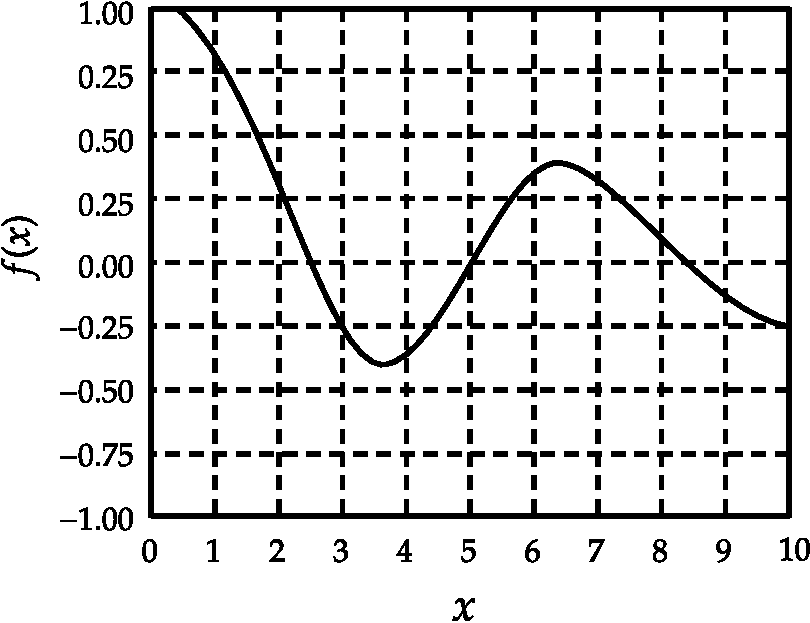
\includegraphics[height=6cm,width=8cm]{diagram-20211005(12)-crop}
	\end{figure}
	\begin{tasks}(2)
		\task[\textbf{A.}]  The Bessel function $J_{0}(x)$
		\task[\textbf{B.}] $\cos x$
		\task[\textbf{C.}] $e^{-x} \cos x$
		\task[\textbf{D.}] $\frac{1}{x} \cos x$
	\end{tasks}
	\item Given that $\sum_{n=0}^{\infty} H_{n}(x) \frac{t^{n}}{n !}=e^{-t^{2}+2 t x}$ the value of $H_{4}(0)$ is
	{\exyear{NET/JRF(JUNE-2013)}}
	\begin{tasks}(4)
		\task[\textbf{A.}] 12
		\task[\textbf{B.}] 6
		\task[\textbf{C.}] 24
		\task[\textbf{D.}] $-6$
	\end{tasks}
	\item   Given $\sum_{n=0}^{\infty} P_{n}(x) t^{n}=\left(1-2 x t+t^{2}\right)^{-1 / 2}$, for $|t|<1$, the value of $P_{5}(-1)$ is
	{\exyear{NET/JRF(JUNE-2014)}}
	\begin{tasks}(4)
		\task[\textbf{A.}] $0.26$
		\task[\textbf{B.}] 1
		\task[\textbf{C.}] $0.5$
		\task[\textbf{D.}] $-1$
	\end{tasks}
	\item The function $f(x)=\sum_{n=0}^{\infty} \frac{(-1)^{n}}{n !(n+1) !}\left(\frac{x}{2}\right)^{2 n+1}$, satisfies the differential equation
	{\exyear{NET/JRF(DEC-2014)}}
	\begin{tasks}(2)
		\task[\textbf{A.}]  $x^{2} \frac{d^{2} f}{d x^{2}}+x \frac{d f}{d x}+\left(x^{2}+1\right) f=0$
		\task[\textbf{B.}]  $x^{2} \frac{d^{2} f}{d x^{2}}+2 x \frac{d f}{d x}+\left(x^{2}-1\right) f=0$
		\task[\textbf{C.}] $x^{2} \frac{d^{2} f}{d x^{2}}+x \frac{d f}{d x}+\left(x^{2}-1\right) f=0$
		\task[\textbf{D.}] $x^{2} \frac{d^{2} f}{d x^{2}}-x \frac{d f}{d x}+\left(x^{2}-1\right) f=0$
	\end{tasks}
	\item
	 The Hermite polynomial $H_{n}(x)$, satisfies the differential equation
	$$
	\frac{d^{2} H_{n}}{d x^{2}}-2 x \frac{d H_{n}}{d x}+2 n H_{n}(x)=0
	$$
	The corresponding generating function $G(t, x)=\sum_{n=0}^{\infty} \frac{1}{n !} H_{n}(x) t^{n}$, satisfies the equation
	{\exyear{NET/JRF(DEC-2015)}}
	\begin{tasks}(2)
		\task[\textbf{A.}] $\frac{\partial^{2} G}{\partial x^{2}}-2 x \frac{\partial G}{\partial x}+2 t \frac{\partial G}{\partial t}=0$
		\task[\textbf{B.}] $\frac{\partial^{2} G}{\partial x^{2}}-2 x \frac{\partial G}{\partial x}-2 t^{2} \frac{\partial G}{\partial t}=0$
		\task[\textbf{C.}] $\frac{\partial^{2} G}{\partial x^{2}}-2 x \frac{\partial G}{\partial x}+2 \frac{\partial G}{\partial t}=0$
		\task[\textbf{D.}]  $\frac{\partial^{2} G}{\partial x^{2}}-2 x \frac{\partial G}{\partial x}+2 \frac{\partial^{2} G}{\partial x \partial t}=0$
	\end{tasks}
	\item A stable asymptotic solution of the equation $x_{n+1}=1+\frac{3}{1+x_{n}}$ is $x=2$. If we take $x_{n}=2+\epsilon_{n}$ and $x_{n+1}=2+\epsilon_{n+1}$, where $\epsilon_{n}$ and $\epsilon_{n+1}$ are both small, the ratio $\frac{\epsilon_{n+1}}{\epsilon_{n}}$ is approximately
	{\exyear{NET/JRF(DEC-2016)}}
	\begin{tasks}(4)
		\task[\textbf{A.}] $-\frac{1}{2}$
		\task[\textbf{B.}] $-\frac{1}{4}$
		\task[\textbf{C.}]  $-\frac{1}{3}$
		\task[\textbf{D.}] $-\frac{2}{3}$
	\end{tasks}
	\item  The Green's function satisfying
	$$
	\frac{d^{2}}{d x^{2}} g\left(x, x_{0}\right)=\delta\left(x-x_{0}\right)
	$$
	with the boundary conditions $g\left(-L, x_{0}\right)=0=g\left(L, x_{0}\right)$, is
	{\exyear{NET/JRF(JUNE-2017)}}
	\begin{tasks}(1)
		\task[\textbf{A.}] $\left\{\begin{array}{ll}\frac{1}{2 L}\left(x_{0}-L\right)(x+L), & -L \leq x<x_{0} \\ \frac{1}{2 L}\left(x_{0}+L\right)(x-L), & x_{0} \leq x \leq L\end{array}\right.$
		\task[\textbf{B.}]  $\left\{\begin{array}{ll}\frac{1}{2 L}\left(x_{0}+L\right)(x+L), & -L \leq x<x_{0} \\ \frac{1}{2 L}\left(x_{0}-L\right)(x-L), & x_{0} \leq x \leq L\end{array}\right.$
		\task[\textbf{C.}] $\left\{\begin{array}{ll}\frac{1}{2 L}\left(L-x_{0}\right)(x+L), & -L \leq x<x_{0} \\ \frac{1}{2 L}\left(x_{0}+L\right)(L-x), & x_{0} \leq x \leq L\end{array}\right.$
		\task[\textbf{D.}] $\frac{1}{2 L}(x-L)(x+L), \quad-L \leq x \leq L$
	\end{tasks}
	\item  The generating function $G(t, x)$ for the Legendre polynomials $P_{n}(t)$ is
	$$
	G(t, x)=\frac{1}{\sqrt{1-2 x t+x^{2}}}=\sum_{n=0}^{\infty} x^{n} P_{n}(t), \text { for }|x|<1
	$$
	If the function $f(x)$ is defined by the integral equation $\int_{0}^{x} f\left(x^{\prime}\right) d x^{\prime}=x G(1, x)$, it can be expressed as
	{\exyear{NET/JRF(DEC-2017)}}
	\begin{tasks}(2)
		\task[\textbf{A.}] $\sum_{n, m=0}^{\infty} x^{n+m} P_{n}(1) P_{m}\left(\frac{1}{2}\right)$
		\task[\textbf{B.}] $\sum_{n, m=0}^{\infty} x^{n+m} P_{n}(1) P_{m}(1)$
		\task[\textbf{C.}] $\sum_{n, m=0}^{\infty} x^{n-m} P_{n}(1) P_{m}(1)$
		\task[\textbf{D.}] $\sum_{n, m=0}^{\infty} x^{n-m} P_{n}(0) P_{m}(1)$
	\end{tasks}
	\item In the function $P_{n}(x) e^{-x^{2}}$ of a real variable $x, P_{n}(x)$ is polynomial of degree $n$. The maximum number of extrema that this function can have is
	{\exyear{NET/JRF(JUNE-2018)}}
	\begin{tasks}(4)
		\task[\textbf{A.}] $n+2$
		\task[\textbf{B.}]  $n-1$
		\task[\textbf{C.}] $n+1$
		\task[\textbf{D.}] $n$
	\end{tasks}
	\item  The Green's function $G\left(x, x^{\prime}\right)$ for the equation $\frac{d^{2} y(x)}{d x^{2}}+y(x)=f(x)$, with the boundary values $y(0)=y\left(\frac{\pi}{2}\right)=0$, is
	{\exyear{NET/JRF(JUNE-2018)}}
	\begin{tasks}(1)
		\task[\textbf{A.}] $G\left(x, x^{\prime}\right)=\left\{\begin{array}{ll}x\left(x^{\prime}-\frac{\pi}{2}\right), & 0<x<x^{\prime}<\frac{\pi}{2} \\ \left(x-\frac{\pi}{2}\right) x^{\prime}, & 0<x^{\prime}<x<\frac{\pi}{2}\end{array}\right.$
		\task[\textbf{B.}] $G\left(x, x^{\prime}\right)=\left\{\begin{array}{ll}-\cos x^{\prime} \sin x, & 0<x<x^{\prime}<\frac{\pi}{2} \\ -\sin x^{\prime} \cos x, & 0<x^{\prime}<x<\frac{\pi}{2}\end{array}\right.$
		\task[\textbf{C.}] $G\left(x, x^{\prime}\right)=\left\{\begin{array}{ll}\cos x^{\prime} \sin x, & 0<x<x^{\prime}<\frac{\pi}{2} \\ \sin x^{\prime} \cos x, & 0<x^{\prime}<x<\frac{\pi}{2}\end{array}\right.$
		\task[\textbf{D.}] $G\left(x, x^{\prime}\right)=\left\{\begin{array}{ll}x\left(\frac{\pi}{2}-x^{\prime}\right), & 0<x<x^{\prime}<\frac{\pi}{2} \\ x^{\prime}\left(\frac{\pi}{2}-x\right), & 0<x^{\prime}<x<\frac{\pi}{2}\end{array}\right.$
	\end{tasks}
	\item The polynomial $f(x)=1+5 x+3 x^{2}$ is written as linear combination of the Legendre polynomials
	$\left(P_{0}(x)=1, P_{1}(x), P_{2}(x)=\frac{1}{2}\left(3 x^{2}-1\right)\right)$ as $f(x)=\sum_{n} c_{n} P_{n}(x)$. The value of $c_{0}$ is
	{\exyear{NET/JRF(DEC-2018)}}
	\begin{tasks}(4)
		\task[\textbf{A.}] $\frac{1}{4}$
		\task[\textbf{B.}] $\frac{1}{2}$
		\task[\textbf{C.}]  2
		\task[\textbf{D.}]  4
	\end{tasks}
	\item The Green's function $G\left(x, x^{\prime}\right)$ for the equation $\frac{d^{2} y(x)}{d x^{2}}=f(x)$, with the boundary values $y(0)=0$ and $y(1)=0$, is
	{\exyear{NET/JRF(DEC-2018)}}
	\begin{tasks}(1)
		\task[\textbf{A.}] $G\left(x, x^{\prime}\right)=\left\{\begin{array}{ll}\frac{1}{2} x\left(1-x^{\prime}\right), & 0<x<x^{\prime}<1 \\ \frac{1}{2} x^{\prime}(1-x) & 0<x^{\prime}<x<1\end{array}\right.$
		\task[\textbf{B.}] $G\left(x, x^{\prime}\right)=\left\{\begin{array}{ll}x\left(x^{\prime}-1\right), & 0<x<x^{\prime}<1 \\ x^{\prime}(1-x) & 0<x^{\prime}<x<1\end{array}\right.$
		\task[\textbf{C.}] $G\left(x, x^{\prime}\right)=\left\{\begin{array}{ll}-\frac{1}{2} x\left(1-x^{\prime}\right), & 0<x<x^{\prime}<1 \\ \frac{1}{2} x^{\prime}(1-x) & 0<x^{\prime}<x<1\end{array}\right.$
		\task[\textbf{D.}]  $G\left(x, x^{\prime}\right)=\left\{\begin{array}{ll}x\left(x^{\prime}-1\right), & 0<x<x^{\prime}<1 \\ x^{\prime}(x-1) & 0<x^{\prime}<x<1\end{array}\right.$
	\end{tasks}
	\item  The Green's function for the differential equation $\frac{d^{2} x}{d t^{2}}+x=f(t)$, satisfying the initial conditions $x(0)=\frac{d x}{d t}(0)=0$ is\\
	$$G(t, \tau)=\left\{\begin{array}{ll}0 & \text { for } \quad 0<t<\tau \\ \sin (t-\tau) & \text { for } \quad t>\tau\end{array}\right.$$\\
	The solution of the differential equation when the source $f(t)=\theta(t)$ (the Heaviside step function) is
	{\exyear{NET/JRF(JUNE-2020)}}
	\begin{tasks}(4)
		\task[\textbf{A.}] $\sin t$
		\task[\textbf{B.}] $1-\sin t$
		\task[\textbf{C.}] $1-\cos t$
		\task[\textbf{D.}] $\cos ^{2} t-1$
	\end{tasks}
\end{enumerate}
 \colorlet{ocre1}{ocre!70!}
\colorlet{ocrel}{ocre!30!}
\setlength\arrayrulewidth{1pt}
\begin{table}[H]
	\centering
	\arrayrulecolor{ocre}
	\begin{tabular}{|p{1.5cm}|p{1.5cm}||p{1.5cm}|p{1.5cm}|}
		\hline
		\multicolumn{4}{|c|}{\textbf{Answer key}}\\\hline\hline
		\rowcolor{ocrel}Q.No.&Answer&Q.No.&Answer\\\hline
		1&\textbf{D} &2&\textbf{D}\\\hline 
		3&\textbf{A} &4&\textbf{A} \\\hline
		5&\textbf{D} &6&\textbf{C} \\\hline
		7&\textbf{A}&8&\textbf{C}\\\hline
		9&\textbf{A}&10&\textbf{B}\\\hline
		11&\textbf{C} &12&\textbf{B}\\\hline
		13&\textbf{C}&14&\textbf{D}\\\hline
		15&\textbf{C}& &\\\hline
		
	\end{tabular}
\end{table}
\begin{abox}
	Problem Set -3
\end{abox}
\begin{enumerate}[label=\color{ocre}\textbf{\arabic*.}]
	\item Green function for time dependent Schrödinger wave equation is defined as $G\left(\vec{r}, t: r^{\prime}, t^{\prime}\right)$. If $H$ is Hamiltonion of system then $G\left(\vec{r}, t: r^{\prime}, t^{\prime}\right)$ will satisfied the equation
	 \begin{tasks}(1)
		\task[\textbf{a.}]$\left(i \hbar \frac{\partial}{\partial t}-H\right) G\left(\vec{r}, t ; \vec{r}^{\prime}, t^{\prime}\right)=0$
		\task[\textbf{b.}]$\left(i \hbar \frac{\partial}{\partial t}-H\right) G\left(\vec{r}, t ; \vec{r}^{\prime}, t^{\prime}\right)=\delta\left(\vec{r}-\vec{r}^{\prime}\right)$
		\task[\textbf{c.}] $\left(i \hbar \frac{\partial}{\partial t}-H\right) G\left(\vec{r}, t ; \vec{r}^{\prime}, t^{\prime}\right)=\delta\left(t-t^{\prime}\right)$
		\task[\textbf{d.}]  $\left(i \hbar \frac{\partial}{\partial t}-H\right) G\left(\vec{r}, t ; \vec{r}^{\prime}, t^{\prime}\right)=\delta\left(\vec{r}-\vec{r}^{\prime}\right) \delta\left(t-t^{\prime}\right)$
	\end{tasks}
\begin{answer}
So the correct answer is \textbf{Option (d)}
\end{answer}
	\item $G\left(x, x_{0}\right)$ is the Green's function associated with the boundary value problem consisting of ordinary differential equation.
	$$
	\frac{d}{d x}\left(p(x) \frac{d u}{d x}\right)=f(x) \text { with } u(0)=0, u(L)=0
	$$
	The discontinuity condition on the derivative $\frac{d G\left(x, x_{0}\right)}{d x}$ at $x=x_{0}$ is
	 \begin{tasks}(4)
		\task[\textbf{a.}]0
		\task[\textbf{b.}]$p\left(x_{0}\right)$
		\task[\textbf{c.}]1
		\task[\textbf{d.}] $\frac{1}{p\left(x_{0}\right)}$
	\end{tasks}
\begin{answer}
	\begin{align*}
	\left.\frac{d G}{d x}\right|_{x=x_{0}^{+}}-\left.\frac{d G}{d x}\right|_{x=x_{i 1}^{-}}=\frac{1}{p\left(x_{0}\right)}
	\end{align*}
	So the correct answer is \textbf{Option (d)}
\end{answer}
\item Consider the steady state heat equation $\frac{d^{2} u}{d x^{2}}=f(x)$ with boundary condition,
$$
u(0)=0, u(L)=0
$$
The Green's function associated with the above equation
 \begin{tasks}(2)
	\task[\textbf{a.}]Constant
	\task[\textbf{b.}] Linear function
	\task[\textbf{c.}] Parabolic function
	\task[\textbf{d.}] Hyperbolic function
\end{tasks}
\begin{answer}
	\begin{align*}
	\intertext{The Green's function satisfies}
	\frac{d^{2} G\left(x, x_{0}\right)}{d x^{2}}&=\delta\left(x-x_{0}\right)\\
\text{	with }G\left(0, x_{0}\right)&=0\text{ and }G\left(L, x_{0}\right)=0
\intertext{Corresponding homogeneous equation is:}
\frac{d^{2} G}{d x^{2}}&=0\\
\text{Solution for }x \neq x_{0}&\text{ are, }G\left(x, x_{0}\right)= \begin{cases}a+b x_{2} & x<x_{1+} \\ c+d x, & x>x_{0}\end{cases}
	\end{align*}
		So the correct answer is \textbf{Option (b)}
\end{answer}
\item Consider the steady state heat equation $\frac{d^{2} u}{d x^{2}}=f(x)$ with boundary condition. $u(0)=0, u(L)=0$
The Green's function associated with the above equation is
 \begin{tasks}(1)
	\task[\textbf{a.}] $G\left(x, x_{0}\right)= \begin{cases}\frac{x}{L}\left(x_{0}-L\right), & 0 \leq x \leq x_{0} \\ \frac{x_{0}}{L}(x-L), & x_{0} \leq x \leq L\end{cases}$
	\task[\textbf{b.}] $G\left(x, x_{0}\right)= \begin{cases}\frac{x}{L}\left(L-x_{0}\right), & 0 \leq x \leq x_{0} \\ \frac{x_{0}}{L}(L-x), & x_{0} \leq x \leq L\end{cases}$
	\task[\textbf{c.}] $G\left(x, x_{0}\right)= \begin{cases}\sqrt{\frac{x}{L},} &\quad 0 \leq x \leq x_{0} \\ \sqrt{\frac{(x-L)}{L}}, & \quad x_{0} \leq x \leq L\end{cases}$
	\task[\textbf{d.}] $G\left(x, x_{0}\right)= \begin{cases}\sqrt{\frac{L-x}{L},}, & 0 \leq x \leq x_{0} \\ \sqrt{\frac{(x)}{L}}, & x_{0} \leq x \leq L\end{cases}$
\end{tasks}
\begin{answer}
	\begin{align*}
	\intertext{The Green's function satisfies}
	\frac{d^{2} G\left(x, x_{0}\right)}{d x^{2}}&=\delta\left(x-x_{0}\right)\\
	\text{with }G\left(0, x_{0}\right)&=0\text{ and }G\left(L, x_{0}\right)=0
	\intertext{Corresponding homogeneous equation is:}
	\frac{d^{2} G}{d x^{2}}&=0\\
	\text{Solution for }&x \neq x_{0}\text{ are}\\
	G\left(x, x_{0}\right)&= \begin{cases}a+b x, & x<x_{0} \\ c+d x, & x>x_{0}\end{cases}
	\intertext{From boundary conditions:}
	G\left(0, x_{0}\right)&=0 \Rightarrow a=0\\
	G\left(L, x_{0}\right)&=0 \Rightarrow c=-d L\\
	\therefore G\left(x, x_{0}\right)&= \begin{cases}b x, & x<x_{0} \\ d(x-L), & x>x_{0}\end{cases}\\
	\text{From continuity of }&\text{Green's function at }x=x_{0},\text{ we have}\\
	b x_{0}&=d\left(x_{0}-L\right)\\
	b&=\frac{d\left(x_{0}-L\right)}{x_{0}}\\
	\text{From discontinuity of }&\frac{\partial G}{\partial x}\text{ at }x=x_{0}\text{, we have}\\
	\left.\frac{\partial G}{\partial x}\right|&_{x=x_{0}^{+}}-\left.\frac{\partial G}{\partial x}\right|_{x=x_{0}^{-}}=1\\
	d-b&=1\\
	\Rightarrow d&=b+1 \Rightarrow d=\frac{d\left(x_{0}-L\right)}{x_{0}}+1 \Rightarrow d x_{0}=d x_{0}-d L+x_{0}\\
	\Rightarrow d&=\frac{x_{0}}{L}, b=d-1=\left(\frac{x_{0}}{L}-1\right)\\
	\therefore G\left(x, x_{0}\right)&= \begin{cases}\frac{x}{L}\left(x_{0}-L\right), & 0 \leq x \leq x_{0} \\ \frac{x_{0}}{L}(x-L), & x_{0} \leq x \leq L\end{cases}
	\end{align*}
		So the correct answer is \textbf{Option (a)}
\end{answer}
\item The differential equation defined as $\frac{d^{2} y}{d x^{2}}=f(x)$ With boundary conditions $\quad y(0)=0$ and $y^{\prime}(1)=0$
The green function $G\left(x, x_{0}\right)$ satisfy the
 \begin{tasks}(2)
	\task[\textbf{a.}]$G\left(x, x_{0}\right)= \begin{cases}x & \text { if } x<x_{0} \\ x_{0} & \text { if } x>x_{0}\end{cases}$
	\task[\textbf{b.}]$G\left(x, x_{0}\right)= \begin{cases}-x & \text { if } x<x_{0} \\ -x_{0} & \text { if } x>x_{0}\end{cases}$
	\task[\textbf{c.}]$G\left(x, x_{0}\right)= \begin{cases}x^{2} & \text { if } x<x_{0} \\ -x_{0} & \text { if } x>x_{0}\end{cases}$
	\task[\textbf{d.}] $G\left(x, x_{0}\right)= \begin{cases}-x^{2} & \text { if } x<x_{0} \\ -x_{0} & \text { if } x>x_{0}\end{cases}$
\end{tasks}
\begin{answer}
	\begin{align}
	\intertext{The corresponding non-homogenous differential equation for Green's function is}\notag\\
	\frac{\partial^{2}}{\partial x^{2}} G\left(x, x_{0}\right)&=\delta\left(x-x_{0}\right)\\
	\text{With }G\left(0, x_{0}\right)&=0\text{ and }G^{\prime}\left(1, x_{0}\right)=0\notag\notag\\
\text{	Let }&\frac{\partial^{2}}{\partial x^{2}} G\left(x, x_{0}\right)=0\notag\\
\Rightarrow G\left(x, x_{0}\right)&= \begin{cases}A x+B, & x<x_{0} \\ C x+D, & x>x_{0}\end{cases}\label{SF-01}
\intertext{Using booundary condition, we have}\notag\\
B&=0\text{ and }C=0\notag\\
\therefore&\text{ equation (\ref{SF-01}) becomes}\notag\\
G\left(x, x_{b}\right)&= \begin{cases}A x, & x<x_{0} \\ D, & x>x_{i 1}\end{cases}\notag\\
\text{From continuity of }&\left(f\left(x, x_{0}\right)\right.\text{ at }x=x_{0}\text{, we have}\notag\\
A x_{0}&=D
\intertext{From discontinuity of first derivative of Green's function i.c. $\frac{\partial G}{\partial x}$ at $x=x_{0}$ we have}
\left.\frac{\partial G}{\partial x}\right|_{x=x_{0}^{+}}-\left.\frac{\partial G}{\partial x}\right|&_{x=x_{0}^{-}}=1\notag\\
\Rightarrow 0-A&=1 \Rightarrow A=-1\notag\\
\text{and }D&=-x_{0}\notag\\
\therefore G\left(x, x_{0}\right)&= \begin{cases}-x & \text { if } x<x_{0} \notag\\ -x_{0} & \text { if } x>x_{0}\end{cases}
	\end{align}
	So the correct answer is \textbf{Option (b)}
\end{answer}
\item For real $n$ the cylindrical Bessel function of order $n$ is $J_{n}(x)$ then $J_{1 / 2}$ will converge to
 \begin{tasks}(4)
	\task[\textbf{a.}]0
	\task[\textbf{b.}]1
	\task[\textbf{c.}] $-1$
	\task[\textbf{d.}] $\frac{1}{2}$
\end{tasks}
\begin{answer}
	\begin{align*}
	{{\color{red}{Not completed}}}\\
	\end{align*}
	So the correct answer is \textbf{Option (a)}
\end{answer}
\item For real $n$ the cylindrical Bessel function is $J_{n}(x)$ of order $n$ then behavior $J_{1 / 2}$ will behave $x \approx 0$ as
 \begin{tasks}(4)
	\task[\textbf{a.}] 0
	\task[\textbf{b.}]$\sqrt{\frac{2 x}{\pi}}$
	\task[\textbf{c.}]$\sqrt{\frac{x}{\pi}}$
	\task[\textbf{d.}]  $\sqrt{\frac{x}{2 \pi}}$
\end{tasks}
\begin{answer}
	\begin{align*}
	{{\color{red}{Not completed}}}\\
	J_{n}(x)&=\sum_{0}^{\infty} \frac{(-1)^{r}}{[r \mid n+r}\left(\frac{x}{2}\right)^{n+2 r} \Rightarrow J_{1 / 2}(x)=\sum_{0}^{\infty} \frac{(-1)^{r}}{\left\lfloor\frac{1}{2}+r\right.}\left(\frac{x}{2}\right)^{\frac{1}{2}+2 r}\\
	\text{Put }r&=0 \frac{\sqrt{x / 2}}{\frac{1}{2}}=\sqrt{\frac{2 x}{\pi}} \text{where }\frac{1}{2}=\frac{\sqrt{\pi}}{2}
	\end{align*}
		So the correct answer is \textbf{Option (b)}
\end{answer}
\item For real $n$ the cylindrical Bessel function is $J_{n}(x)$ of order $n$ then behavior $J_{1 / 2}$ will equivalent to (it is given that $\underline{r} \cdot\left\lfloor r-\frac{1}{2}=\left[(2 r) 2^{-r} \sqrt{\pi}\right)\right.$
 \begin{tasks}(4)
	\task[\textbf{a.}] $\sqrt{\frac{2}{\pi}} \frac{\sin x}{\sqrt{x}}$
	\task[\textbf{b.}]$\sqrt{\frac{2}{\pi}} \frac{\sin x}{x}$
	\task[\textbf{c.}]$\sqrt{\frac{2}{\pi}} \frac{\cos x}{\sqrt{x}}$
	\task[\textbf{d.}] $\sqrt{\frac{2}{\pi}} \frac{\cos }{x}$
\end{tasks} 
\begin{answer}
	\begin{align*}
	{{\color{red}{Not completed}}}\\
	\end{align*}
\end{answer}
\item For real $n$ the cylindrical Bessel function is $J_{n}(x)$ of order $n$ then $J_{n}(x)$ will satisfied differential equation
 \begin{tasks}(1)
	\task[\textbf{a.}]$\frac{d^{2} J_{n}}{d x^{2}}+\frac{1}{x}\left(\frac{d J_{n}}{d x}\right)+\left(1+\frac{n^{2}}{x^{2}}\right) J_{n}=0$
	\task[\textbf{b.}] $\frac{d^{2} J_{n}}{d x^{2}}+\frac{1}{x}\left(\frac{d J_{n}}{d x}\right)+\left(1-\frac{n^{2}}{x^{2}}\right) J_{n}=0$
	\task[\textbf{c.}] $\frac{d^{2} J_{n}}{d x^{2}}+x\left(\frac{d J_{n}}{d x}\right)+\left(1+\frac{n^{2}}{x^{2}}\right) J_{n}=0$
	\task[\textbf{d.}] $\frac{d^{2} J_{n}}{d x^{2}}+x\left(\frac{d J_{n}}{d x}\right)+\left(1-\frac{n^{2}}{x^{2}}\right) J_{n}=0$
\end{tasks}
\begin{answer}
	\begin{align*}
\text{The Bessel function is given by }\frac{d^{2} J_{n}}{d x^{2}}+\frac{1}{x}\left(\frac{d J_{n}}{d x}\right)+\left(1-\frac{n^{2}}{x^{2}}\right) J_{n}=0
	\end{align*}
		So the correct answer is \textbf{Option (b)}
\end{answer}
\item For real $n$ the cylindrical Bessel function is $J_{n}(x)$ of order $n$ then value of $\frac{d J_{0}}{d x}$ is equivalent to 
 \begin{tasks}(4)
	\task[\textbf{a.}] $J_{1}$
	\task[\textbf{b.}]$-J_{1}$
	\task[\textbf{c.}]$2 J_{1}$
	\task[\textbf{d.}]$-2 J_{1}$
\end{tasks}
\begin{answer}
	\begin{align*}
J_{n+1}(x)=-J_{n}^{\prime}(x)+\frac{n}{x} J_{n}\text{. for }n=0, J_{1}=-J_{0}^{\prime}
	\end{align*}
		So the correct answer is \textbf{Option (b)}
\end{answer}
\item  The differential equation $x^{2} \frac{d^{2} y}{d x^{2}}+2 x \frac{d y}{d x}+\left[x^{2}-\lambda\right] y(x)=0$ is spherical Bessel's differential equation of order $n$ then value of $\lambda$ is given by
 \begin{tasks}(4)
	\task[\textbf{a.}]$n$
	\task[\textbf{b.}]$n(n+1)$
	\task[\textbf{c.}] $n(n-1)$
	\task[\textbf{d.}]  $n^{2}$
\end{tasks}
\begin{answer}
	\begin{align*}
\text{Spherical Bessel's differential equation }x^{2} \frac{d^{2} y}{d x^{2}}+2 x \frac{d y}{d x}+\left[x^{2}-n(n+1)\right] y(x)=0
	\end{align*}
		So the correct answer is \textbf{Option (b)}
\end{answer}
\item If $J_{n}(x)$ is spherical Bessel function of order $n$ if $N_{n}(x)$ is spherical Neumann function of order $n$ and $h_{n}^{\prime}$ is spherical Hankel function of type one of order $n$. Then $h_{0}^{1}$ is given by
 \begin{tasks}(4)
	\task[\textbf{a.}]$i \frac{e^{-i x}}{x}$
	\task[\textbf{b.}]$-i \frac{e^{-i x}}{x}$
	\task[\textbf{c.}] $i \frac{e^{i x}}{x}$
	\task[\textbf{d.}] $-i \frac{e^{i x}}{x}$
\end{tasks}
\begin{answer}
	\begin{align*}
		h_{n}^{1}&=J_{n}+i N_{n}\\
	J_{0}(x)&=\frac{\sin x}{x}, N_{0}(x)=-\frac{\cos x}{x} \Rightarrow h_{0}^{\prime^{\prime}}=J_{0}+i N_{0}=\frac{\sin x-i \cos x}{\because x}=-i \frac{e^{i x}}{x}
	\end{align*}
	So the correct answer is \textbf{Option (d)}
\end{answer}
\item If $J_{n}(x)$ is spherical Bessel function of order $n$ if $N_{n}(x)$ is spherical Neumann function of order $n$ and $h_{n}^{2}$ is spherical Hankel function of type two of order $n$. Then $h_{0}^{2}$ is given by
 \begin{tasks}(4)
	\task[\textbf{a.}] $i \frac{e^{-i x}}{x}$
	\task[\textbf{b.}] $-i \frac{e^{-i x}}{x}$
	\task[\textbf{c.}]$i \frac{e^{i x}}{x}$
	\task[\textbf{d.}] $-i \frac{e^{i x}}{x}$
\end{tasks}
\begin{answer}
	\begin{align*}
	h_{n}^{2}&=J_{n}-i N_{n}\\
	J_{0}(x)&=\frac{\sin x}{x},N_{0}(x)=-\frac{\cos x}{x} \Rightarrow h_{0}^{1}=J_{0}+i N_{0} \Rightarrow \frac{\sin x+i \cos x}{x}=i \frac{e^{-i x}}{x}
	\end{align*}
		So the correct answer is \textbf{Option (a)}
\end{answer}
\item If $J_{n}(x)$ is spherical Bessel function of order $n$ then $j_{0}^{\prime}(x)$ is equivalent to
 \begin{tasks}(4)
	\task[\textbf{a.}]$j_{1}(x)$
	\task[\textbf{b.}]$-j_{1}(x)$
	\task[\textbf{c.}]$\frac{j_{1}(x)}{2}$
	\task[\textbf{d.}]$-\frac{j_{1}(x)}{2}$
\end{tasks}
\begin{answer}
	\begin{align*}
	\frac{d}{d x}\left(j_{0}(x)\right)&=\frac{d}{d x}\left(\frac{\sin x}{x}\right)=\frac{\cos x}{x}-\frac{\sin x}{x^{2}}=-J_{1}(x)\\
	\text{Where }j_{1}(x)&=-\frac{\cos x}{x}+\frac{\sin x}{x^{2}}
	\end{align*}
	So the correct answer is \textbf{Option (b)}
\end{answer}
\item The solution of the differential equation $x^{2} \frac{d^{2} y}{d x^{2}}+2 x \frac{d y}{d x}+x^{2} y(x)=0$ subjected to the condition is given by $y(0)=1$.
 \begin{tasks}(4)
	\task[\textbf{a.}] $\frac{\sin x}{x}$
	\task[\textbf{b.}] $\frac{\cos x}{x}$
	\task[\textbf{c.}]$\frac{\exp (-i x)}{x}$
	\task[\textbf{d.}] $\frac{\exp i x}{x}$
\end{tasks}
\begin{answer}
	\begin{align*}
 \text{Spherical Bessel's differential equation }&x^{2} \frac{d^{2} y}{d x^{2}}+2 x \frac{d y}{d x}+\left[x^{2}-n(n+1)\right] y(x)=0\\
 \text{ then }x^{2} \frac{d^{2} y}{d x^{2}}+2 x \frac{d y}{d x}+x^{2} y(x)=0 &\text{ is spherical Bessel's differential equation for order}\\
 n&=0\\
	\text{then solution is }J_{0}(x)&=\frac{\sin x}{x}\text{ with boundary condition }y(0)=1.
	\end{align*}
	So the correct answer is \textbf{Option (a)}
\end{answer}
\item $H_{n}(x)$ is Hermite polynomials of order $n$ then $H_{n}(x)=(-1)^{n} f(x) \frac{d^{n}(W(x))}{d x^{n}}$, then $f(x)$ and $W(x)$ are respectively
 \begin{tasks}(1)
	\task[\textbf{a.}]$f(x)=\exp \left(x^{2}\right), W(x)=\exp \left(-x^{2}\right)$
	\task[\textbf{b.}]$f(x)=\exp \left(-x^{2}\right), W=\exp \left(x^{2}\right)$
	\task[\textbf{c.}] $f(x)=W(x)=\exp \left(x^{2}\right)$
	\task[\textbf{d.}] $f(x)=W(x)=\exp \left(-x^{2}\right)$
\end{tasks}
\begin{answer}
	\begin{align*}
	H_{n}(x)&=(-1)^{n} \exp \left(x^{2}\right) \frac{d^{n}\left(\exp \left(-x^{2}\right)\right)}{d x^{n}}\\
	\text{So after comparing }H_{n}(x)&=(-1)^{n} f(x) \frac{d^{n}(W(x))}{d x^{n}}\\
	f(x)&=\exp \left(x^{2}\right), W(x)=\exp \left(-x^{2}\right)
	\end{align*}
		So the correct answer is \textbf{Option (a)}
\end{answer}
\item The solution of differential equation $\frac{d^{2} y}{d x^{2}}-2 x \frac{d y}{d x}+\lambda y(x)=0$ is Hermilte polynomial of order $n$ then value of $\lambda$ is
 \begin{tasks}(4)
	\task[\textbf{a.}]$n$
	\task[\textbf{b.}] $-n$
	\task[\textbf{c.}]$2 n$
	\task[\textbf{d.}] $-2 n$
\end{tasks}
\begin{answer}
	\begin{align*}
	\frac{d^{2} y}{d x^{2}}-2 x \frac{d y}{d x}+2 n y(x)=0\text{ is Hermite differential equation}
	\end{align*}
		So the correct answer is \textbf{Option (c)}
\end{answer}
\item The Rodrigues formula for Laguerre polunomial is given by
 \begin{tasks}(2)
	\task[\textbf{a.}]$L_n(x)=\frac{e^{-x}}{n !}\left(\frac{d}{d x}\right)^{n}\left(x^{n} e^{-x}\right)$
	\task[\textbf{b.}]$L_{n}(x)=\frac{e^{x}}{n !}\left(\frac{d}{d x}\right)^{n}\left(x^{n} e^{x}\right)$
	\task[\textbf{c.}]$L_n(x)=\frac{e^{-x}}{n !}\left(\frac{d}{d x}\right)^{n}\left(x^{n} e^{x}\right)$
	\task[\textbf{d.}] $L_{n}(x)=\frac{e^{x}}{n !}\left(\frac{d}{d x}\right)^{n}\left(x^{n} e^{-x}\right)$
\end{tasks}
\begin{answer}
	\begin{align*}
	L_{n}(x)=\frac{e^{x}}{n !}\left(\frac{d}{d x}\right)^{n}\left(x^{n} e^{-x}\right)
	\end{align*}
		So the correct answer is \textbf{Option (d)}
\end{answer}
\item It is given that operator $x-\frac{d}{d x}=-\exp \left(\frac{x^{2}}{2}\right) \frac{d}{d x} \exp \left(-\frac{x^{2}}{2}\right)$
If then the normalized wave function for harmonic oscillation is $\psi(x)=\left(\pi^{1 / 2} 2^{n}\lfloor n)^{-1 / 2} \exp \left(-\frac{x^{2}}{2}\right) H_{n}(x)\right.$, then $\psi_n(x)$ is equivalent to 
 \begin{tasks}(1)
	\task[\textbf{a.}]$\psi_{n}(x)=\left(\pi^{1 / 2} 2^{n}\lfloor n)^{-1 / 2}\left(x-\frac{d}{d x}\right)^{n} \exp \left(-\frac{x^{2}}{2}\right)\right.$
	\task[\textbf{b.}] $\psi_{n}(x)=\left(\pi^{1 / 2} 2^{n}\lfloor n)^{-1 / 2}\left(x-\frac{d}{d x}\right)^{2 n} \exp \left(\frac{x^{2}}{2}\right)\right.$
	\task[\textbf{c.}] $\psi_{n}(x)=\left(\pi^{1 / 2} 2^{n}\lfloor n)^{-1 / 2}\left(x-\frac{d}{d x}\right)^{n} \exp \left(-x^{2}\right)\right.$
	\task[\textbf{d.}] $\psi_{n}(x)=\left(\pi^{k / 2} 2^{n}\lfloor n)^{-1 / 2}\left(x-\frac{d}{d x}\right)^{2 n} \operatorname{cxp}\left(-x^{2}\right)\right.$
\end{tasks}
\begin{answer}
	\begin{align*}
	H_{n}(x)&=(-1)^{n} \exp \left(x^{2}\right) \frac{d^{n}\left(\exp \left(-x^{2}\right)\right)}{d x^{n}}\\
	x-\frac{d}{d x} &=-\exp \left(\frac{x^{2}}{2}\right) \frac{d}{d x} \exp \left(-\frac{x^{2}}{2}\right) \Rightarrow\left(x-\frac{d}{d x}\right) \exp \left(-\frac{x^{2}}{2}\right) \\ &\left.=-\exp \left(\frac{x^{2}}{2}\right) \frac{d}{d x} \exp \left(-\frac{x^{2}}{2}\right)\right) \exp \left(-\frac{x^{2}}{2}\right)\\
	x \exp \left(-\frac{x^{2}}{2}\right)-\frac{d \exp \left(-\frac{x^{2}}{2}\right)}{d x}&=-\exp \left(\frac{x^{2}}{2}\right) \frac{d}{d x} \exp \left(-x^{2}\right)\\
	\Rightarrow\left(x-\frac{d}{d x}\right) \exp \left(-\frac{x^{2}}{2}\right)&=\exp \left(\frac{x^{2}}{2}\right)\left(-2 x \exp \left(-x^{2}\right)\right)=2 x \exp -\frac{x^{2}}{2}=H_{1}\left(\exp -\frac{x^{2}}{2}\right)\\
	\text{where }2 x&=H_{1}(x)\\
	\text{Similarly }\left(x-\frac{d}{d x}\right)^{n} \exp \left(-\frac{x^{2}}{2}\right)&=H_{n} \exp \left(-\frac{x^{2}}{2}\right)\\
	\psi_{n}(x)&=\left(\pi^{1 / 2} 2^{n}\lfloor n)^{-1 / 2}\left(x-\frac{d}{d x}\right)^{n} \exp \left(-\frac{x^{2}}{-2}\right)\right.
	\end{align*}
	So the correct answer is \textbf{Option (a)}
\end{answer}
\item The solution of differential equation $x \frac{d^{2} y}{d x^{2}}+(1-x) \frac{d y}{d x}+\lambda y(x)=0$ is Laguerre polynomials of order $n$ then value of $\lambda$ is
 \begin{tasks}(4)
	\task[\textbf{a.}]$n$
	\task[\textbf{b.}]$-n$
	\task[\textbf{c.}] $2 n$
	\task[\textbf{d.}] $-2 n$
\end{tasks}
\begin{answer}
	\begin{align*}
	x \frac{d^{2} y}{d x^{2}}+(1-x) \frac{d y}{d x}+n y(x)=0\text{ is Laguerre differential equation.}
	\end{align*}
	So the correct answer is \textbf{Option (a)}
\end{answer}
\item The generating function $F(x, t)=\sum_{n=0}^{\infty} P_{n}(x) t^{n}$ for the Legendre polynomials $P_{n}(x)$ is $F(x, t)=\left(1-2 x t+t^{2}\right)^{-1 / 2}$. The value of $P_{2}(-1)$ is
 \begin{tasks}(4)
	\task[\textbf{a.}]$5 / 2$
	\task[\textbf{b.}]$3 / 2$
	\task[\textbf{c.}] $+1$
	\task[\textbf{d.}] $-1$
\end{tasks}
\begin{answer}
	\begin{align*}
	\text{The generating function for Legendre polynomial is }F(x, t)&=\left(1-2 x t+t^{2}\right)^{-1 / 2}.\text{ Thus}\\P_{2}(x)=\frac{1}{2}\left(3 x^{2}-1\right) \Rightarrow P_{2}(-1)=\frac{1}{2}(3-1)=1
	\end{align*}
		So the correct answer is \textbf{Option (c)}
\end{answer}
\item If we observe plot of Bessel functions $J_{0}(x), J_{1}(x)$, and $J_{2}(x)$ we find their maxima at $x_{0}, x_{1}$ and $x_{2}$ respectively. Then which of the following is true
 \begin{tasks}(2)
	\task[\textbf{a.}]$x_{0}<x_{1}<x_{2}$
	\task[\textbf{b.}]$x_{0}>x_{1}>x_{2}$
	\task[\textbf{c.}]$x_{0}<x_{1}=x_{2}$
	\task[\textbf{d.}] $x_{0}=x_{1}<x_{2}$
\end{tasks}
\begin{answer}
	So the correct answer is \textbf{Option (a)}
\end{answer}
\item Which one of the following is correctly matched?\\
\begin{figure}[H]
	\centering
	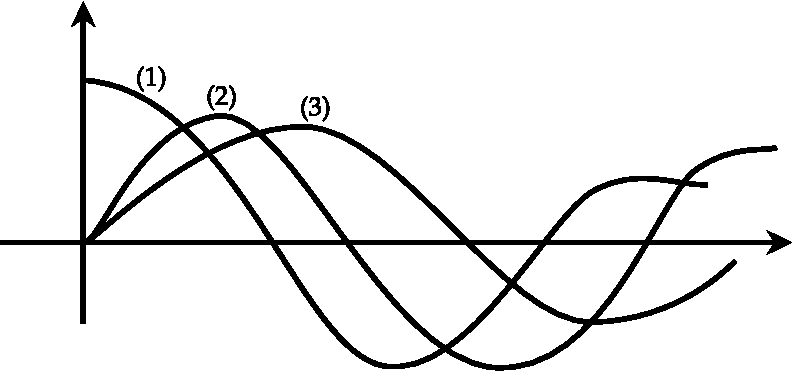
\includegraphics[height=3.5cm,width=6.5cm]{SF-01}
\end{figure}
 \begin{tasks}(2)
	\task[\textbf{a.}](1) $J_{0}$,
	(2) $J_{2}$, (3) $J_{1}$
	\task[\textbf{b.}]$(1) J_{0}$,
	(2) $J_{1}, \quad(3) J_{2}$
	\task[\textbf{c.}](1) $J_{2}$,
	(2) $J_{1}$,
	(3) $J_{0}$
	\task[\textbf{d.}] None of the above
\end{tasks}
\begin{answer}
	So the correct answer is \textbf{Option (b)}
\end{answer}
\item If the generating function of Legendre polynomial is $\frac{1}{\sqrt{1-6 t+t^{2}}}$, then coefficient of $t^{2}$ is
 \begin{tasks}(4)
	\task[\textbf{a.}] 11
	\task[\textbf{b.}]$-11$
	\task[\textbf{c.}]13
	\task[\textbf{d.}] $-13$
\end{tasks}
\begin{answer}
	\begin{align*}
	\intertext{The generating function for the polynomial solutions of the Legendre ODE is given by}
	g(x, t)&=\frac{1}{\sqrt{1-2 x t+t^{2}}}=\sum_{n=0}^{\infty} P_{n}(x) t^{n}\\
	\text{Thus }x&=3\text{ and }n=2.\\
	P_{2}(x)&=\frac{1}{2}\left(3 x^{2}-1\right) \Rightarrow P_{2}(3)=\frac{1}{2}\left(3 \times 3^{2}-1\right)=13
	\end{align*}
		So the correct answer is \textbf{Option (c)}
\end{answer}
\item Which of the following relation is true for Bessel's differential equation?
 \begin{tasks}(2)
	\task[\textbf{a.}]$J_{0}^{\prime}(x)=J_{1}(x)$
	\task[\textbf{b.}]$J_{0}^{\prime}(x)=-J_{2}(x)$
	\task[\textbf{c.}]$J_{0}^{\prime}(x)=J_{2}(x)$
	\task[\textbf{d.}] $J_{0}^{\prime}(x)=-J_{1}(x)$
\end{tasks}
\begin{answer}
	So the correct answer is \textbf{Option (d)}
\end{answer}
\item Given that $\sum_{n=0}^{\infty} H_{n}(x) \frac{t^{n}}{n !}=e^{-t^{2}+2 x x}$ the value of $H_{6}(0)$ is
 \begin{tasks}(4)
	\task[\textbf{a.}]$-120$
	\task[\textbf{b.}]$+120$
	\task[\textbf{c.}]12
	\task[\textbf{d.}]  $-12$
\end{tasks}
\begin{answer}
	\begin{align*}
	\sum_{n=0}^{\infty} I_{n}(x) \frac{t^{\prime \prime}}{n !}&=e^{-t^{2}+2 t x} \Rightarrow \sum_{n=0}^{\infty} H_{n}(0) \frac{t^{n}}{n !}=e^{-t^{2}}=1-t^{2}+\frac{t^{4}}{2 !}-\frac{t^{6}}{3 !}\\
	\Rightarrow \frac{H_{6}(0)}{6 !} t^{6}&=-\frac{1}{3 !} t^{6} \Rightarrow H_{6}(0)=-\frac{6 !}{3 !}=-120
	\end{align*}
	So the correct answer is \textbf{Option (a)}
\end{answer}
\item Given that $\sum_{n=0}^{\infty} H_{n}(x) \frac{t^{n}}{n !}=e^{-t^{2}+2 e x}$ the value of $H_{4}(0)$ is
 \begin{tasks}(4)
	\task[\textbf{a.}]12
	\task[\textbf{b.}] 6
	\task[\textbf{c.}]24
	\task[\textbf{d.}] $-6$
\end{tasks}
\begin{answer}
	\begin{align*}
	\sum_{n=0}^{\infty} H_{n}(x) \frac{t^{n}}{n !}&=e^{-t^{2}+2 t x} \Rightarrow \sum_{n=0}^{\infty} H_{n}(0) \frac{t^{n}}{n !}=e^{-t^{2}}=1-t^{2}+\frac{t^{4}}{2 !}-\frac{t^{6}}{3 !}\\
	\Rightarrow \frac{H_{4}(0)}{4 !} t^{4}&=\frac{t^{4}}{2 !} \Rightarrow H_{4}(0)=\frac{4 !}{2 !}=12
	\end{align*}
	So the correct answer is \textbf{Option (a)}
\end{answer}
\item If Hermite polynomial of order 2 is given by $H_{2}(x)=a x^{2}-2 ; a>0$, then the value of $a$ is
 \begin{tasks}(4)
	\task[\textbf{a.}]3
	\task[\textbf{b.}]4
	\task[\textbf{c.}]5
	\task[\textbf{d.}] 6
\end{tasks}
\begin{answer}
	\begin{align*}
	\intertext{Orthonormality condition,}
	\int_{-\infty}^{+\infty}\left[H_{n}(x)\right]^{2} e^{-x^{2}} d x&=2^{\prime \prime} n ! \sqrt{\pi}\\
	\text{For, }n&=2, \int_{-\infty}^{+\infty}\left(a x^{2}-2\right)^{2} e^{-x^{2}} d x=8 \sqrt{\pi}\\
\text{	Now}
	\int_{-\infty}^{+\infty}\left[H_{2}(x)\right]^{2} e^{-x^{2}} d x&=\int_{-\infty}^{+\infty}\left(a x^{2}-2\right)^{2} e^{-x^{2}} d x=\left\{a^{2} \times \frac{3}{4}+4-2 a\right\} \sqrt{\pi}
	\intertext{Thus, we have}
	\frac{3 a^{2}}{4}+4-2 a&=8 \Rightarrow 3 a^{2}-8 a-16=0 \Rightarrow 3 a^{2}-12 a+4 a-16=0\\
	\Rightarrow 3 a(a-4)+4(a-4)&=0 \Rightarrow(3 a+4)(a-4)=0\\
	\text{Thus, }a&=4
	\end{align*}
		So the correct answer is \textbf{Option (b)}
\end{answer}
\item The value of Legendre polynomial $p_{n}(x)$ for odd $n$ and $x=0$. i.e., $p_{n}(0)$ is
 \begin{tasks}(4)
	\task[\textbf{a.}]1
	\task[\textbf{b.}]0
	\task[\textbf{c.}]$-1$
	\task[\textbf{d.}]  $0.5$
\end{tasks}
\begin{answer}
	\begin{align*}
	\intertext{The generating function for Legendre polynomial is}
	\left(1-2 x t+t^{2}\right)^{-1 / 2}&=\sum_{n=0}^{\infty} p_{n}(x) t^{n}\\
	\text{Put, $x=0$, we get, }&\left(1+t^{2}\right)^{-1 / 2}=\sum p_{n}(\theta) t^{n}
	\end{align*}
		So the correct answer is \textbf{Option (b)}
\end{answer}
\item For the Legendre's polynomial $P_{n}(x)$, given below are two statements. Study these carefully and pick out the correct option.\\
Statement I: $\quad \int_{-1}^{1} x\left[P_{n}(x)\right]^{2} d x=0$\\
Statement I: $\lim _{n \rightarrow \infty}\left[\int_{-1}^{1} x P_{n}(x) P_{n+1}(x) d x\right]=0$
 \begin{tasks}(1)
	\task[\textbf{a.}]Only statement (I) is correct
	\task[\textbf{b.}]Only statement (II) is correct
	\task[\textbf{c.}]Both (I) and (II) are correct
	\task[\textbf{d.}]Neither (I) nor (II) is correet
\end{tasks}
\begin{answer}
	\begin{align*}
	\intertext{From recurrence relation we have}
	(n+1) P_{n+1}(x)&=(2 n+1) x p_{n}(x)-n p_{n-1}(x)\\
	x p_{n}(x)&=\frac{1}{(2 n+1)}\left\{(n+1) p_{n+1}(x)+n p_{n-1}(x)\right\}\\
	x\left[p_{n}(x)\right]^{2}&=\frac{1}{(2 n+1)}\left\{(n+1) p_{n}(x) p_{n+1}(x)+n p_{n}(x) p_{n-1}(x)\right\}\\
	\therefore \int_{-1}^{+1} x\left[p_{n}(x)\right]^{2} d x&=0\left\{\because \int_{-1}^{+1} p_{m}(x) p_{n}(x)=0\right.\text{ if }\left.m \neq n\right\}\\
	\therefore &\int_{-1}^{+1} x\left[p_{n}(x)\right]^{2} d x=0
	\intertext{From recurrence relation, we have}
	(n+1) p_{n+1}(x)&=(2 n+1) x p_{n}(x)-n p_{n-1}(x)\\
	(2 n+1) x p_{n}(x)&=(n+1) p_{n+1}(x)+n p_{n-1}(x)\\
	\int_{-1}^{+1}(2 n+1) x p_{n}(x) p_{n+1}(x) d x&=\int_{-1}^{+1}\left[(n+1)\left\{p_{n+1}(x)\right\}^{2}+n p_{n-1}(x) p_{n+1}(x)\right] d x\\
	=\int_{-1}^{+1}(n+1)\left\{p_{n+1}(x)\right\}^{2} d x+n \int_{-1}^{+1}& p_{n-1}(x) p_{n+1}(x) d x=(n+1) \frac{2}{2(n+1)+1}+0=\frac{2 n+2}{2 n+3}\\
	\therefore \int_{-1}^{+1} x p_{n}(x) p_{n+1}(x) d x&=\frac{2 n+2}{(2 n+1)(2 n+3)}\\
	\lim _{n \rightarrow \infty} \frac{n\left(2+\frac{2}{n}\right)}{n^{2}\left(2+\frac{1}{n}\right)\left(2+\frac{3}{n}\right)}&=\lim _{n \rightarrow \infty} \frac{\left(2+\frac{2}{n}\right)}{n\left(2+\frac{1}{n}\right)\left(2+\frac{3}{n}\right)}=0
	\end{align*}
		So the correct answer is \textbf{Option (c)}
\end{answer}
\item Which of the following statements is Incorrect about the Hermite polynomials $H_{n}(x)$ ?
 \begin{tasks}(1)
	\task[\textbf{a.}] The value of integral $\frac{1}{\sqrt{\pi}} \int_{-\infty}^{\infty} e^{-x^{2}}\left[H_{4}(x)\right]^{2} d x$ is 384
	\task[\textbf{b.}] Hermite polynomial of order $3, H_{3}(x)$, satisfies the differential equation $y^{\prime \prime}-2 x y^{\prime}+6 y=0$
	\task[\textbf{c.}] The value of $\mathrm{H}_{4}(\mathrm{l})$ is $-20$
	\task[\textbf{d.}] $H_{n}(x)=\frac{H_{n+1}(x)+2 n H_{n-1}(x)}{x}$
\end{tasks}
\begin{answer}
	\begin{align*}
	\intertext{When integrated with respect to weight function $e^{-x^{2}}$, the Hermite polynomials satisfy}
	\int_{-\infty}^{\infty} e^{-x^{2}} H_{n}(x) H_{m}(x) d x&= \begin{cases}0, & n \neq m \\ \sqrt{\pi} 2^{n} n !, & n=m\end{cases}
	\intertext{In our case $n=m=4$, hence}
	\frac{1}{\sqrt{\pi}} \int_{-\infty}^{\infty} e^{-x^{2}}\left[H_{4}(x)\right]^{2} d x&=\frac{\sqrt{\pi} 2^{4}(4 !)}{\sqrt{\pi}}=384
	\intertext{Hermite polynomial of order $n$, satisfies the differential equation}
	y^{\prime \prime}-2 x y^{\prime}+2 n y=0\\
\text{	when }n=3, y^{\prime \prime}-2 x y^{\prime}+6 y=0\\
	\text{We have }H_{4}(x)&=16 x^{4}-48 x^{2}+12\\
	\text{Therefore, }H_{4}(1)&=-48+28=-20
	\intertext{The recursion relation for Hermite polynomials is}
	H_{n+1}(x)&=2 x H_{n}(x)-2 n H_{n-1}(x) \Rightarrow H_{n}(x)=\frac{H_{n+1}(x)+2 n H_{n-1}(x)}{2 x}
	\end{align*}
		So the correct answer is \textbf{Option (d)}
\end{answer}
\item If $P_{n}(x)$ denotes the Legendre polynomials of order $n$, then which of the following statements is incorrect?
 \begin{tasks}(1)
	\task[\textbf{a.}]$P_{n}(x)=\frac{1}{2^{n} n !} \frac{d^{n}}{d x^{n}}\left[\left(x^{2}-1\right)^{n}\right]$ where $n=0,1,2 \ldots$
	\task[\textbf{b.}]The Legendre polynomials satisfy the differential equation\\$
	\left(1-x^{2}\right) \frac{d^{2} y}{d x^{2}}-2 x \frac{d y}{d x}+n(n+1) y=0
	$
	\task[\textbf{c.}] For each value of $n$ the Legendre polynomials satisfy the relation $P_{n}(1)=1$.
	\task[\textbf{d.}] The value of integral $\int_{-1}^{1}\left[P_{4}(x)\right]^{2} d x$ is $\frac{2}{7}$.
\end{tasks}
\begin{answer}
	\begin{align*}
	\intertext{Option (a) is the correct definition of Legendre polynomial. Legendre polynoimials satisfy the differential equation given in option (b). For each value of $n$ Legendre polynomials satisfy $P_{n}(1)=1$.}
	\text{Since, }\int_{-1}^{1}\left[P_{n}(x)\right]^{2} d x&=\frac{2}{2 n+1}\\
	\text{Hence, }\int_{-1}^{1}\left[P_{4}(x)\right]^{2} d x&=\frac{2}{2 \cdot 4+1}=\frac{2}{9}\\
	\text{Hence option }&(d)\text{ is incorrect.}
	\end{align*}
		So the correct answer is \textbf{Option (d)}
\end{answer}
\end{enumerate}
%\chapter{Fourier Transform}
\begin{enumerate}
	\item Let $F(k)$ is the Fourier exponential transform of $f(x)$ and $G(k)$ be the Fourier Transform of $g(x)=f(x+a)$. Then $G(k)$ is given by
	(Use the Fourier integral $F(k)=\frac{1}{\sqrt{2 \pi}} \int_{-\infty}^{+\infty} f(x) e^{i k x} d x$ )
	 \begin{tasks}(2)
		\task[\textbf{a.}]$e^{i a k} f(k)$
		\task[\textbf{b.}]$e^{-i a k} F(-k)$
		\task[\textbf{c.}] $e^{-i a k} F(k)$
		\task[\textbf{d.}] $e^{-i a k} f(k)$
	\end{tasks}
	\item The value of a function is given by $f(x)=\left\{\begin{array}{cc}1 & 0<x<1 \\ -1 & 1<x<2 \\ 0 & x>2\end{array}\right.$, the Fourier cosine transform of $f(x)$ is
	 \begin{tasks}(2)
		\task[\textbf{a.}]$\sqrt{\frac{2}{\pi}}\left(\frac{2 \sin \omega+\sin 2 \omega}{\omega}\right)$
		\task[\textbf{b.}]$\sqrt{\frac{2}{\pi}}\left(\frac{2 \sin \omega-\sin 2 \omega}{\omega}\right)$
		\task[\textbf{c.}]$\sqrt{\frac{2}{\pi}}\left(\frac{\sin \omega-\sin 2 \omega}{\omega}\right)$
		\task[\textbf{d.}] $\sqrt{\frac{2}{\pi}}\left(\frac{2 \sin \omega}{\omega}\right)$
	\end{tasks}
	\item Consider the function $\delta_{n}(x)=\frac{n}{\sqrt{\pi}} \exp \left(-n^{2} x^{2}\right)$. For $n \rightarrow \infty$ The Fourier transform of the function is given by
	 \begin{tasks}(2)
		\task[\textbf{a.}]$\delta(x)=\int_{-\infty}^{+\infty} e^{-i k x} d k$
		\task[\textbf{b.}]$\delta(x)=\frac{1}{2 \pi} \int_{-\infty}^{+\infty} e^{i k x} d k$
		\task[\textbf{c.}]$\delta(x)=\frac{1}{2 \pi} \int_{-\infty}^{+\infty} e^{-i k x} d k$
		\task[\textbf{d.}] 0
	\end{tasks}
	\item For the function $f(t)=\delta(t-x)$, the Fourier cosine integral is defined as $g_{c}(\omega)=\sqrt{\frac{2}{\pi}} \int_{0}^{\infty} f(t) \cos \omega t d t$. Its Fourier transform is:
	 \begin{tasks}(2)
		\task[\textbf{a.}] $\sqrt{\frac{2}{\pi}} \cos \omega x$
		\task[\textbf{b.}]$\sqrt{\frac{2}{\pi}}$
		\task[\textbf{c.}]$\sqrt{\frac{2}{\pi}} \sin \omega x$
		\task[\textbf{d.}] $i \sqrt{\frac{2}{\pi}}$
	\end{tasks}
	\item Inverse cosine transform of $g_{c}(\omega)=\sqrt{\frac{2}{\pi}} \cos \omega x$ is:
	 \begin{tasks}(2)
		\task[\textbf{a.}]$\delta(t+x)$
		\task[\textbf{b.}]$\delta(t-x)$
		\task[\textbf{c.}]$\delta(t-x)(t+x)$
		\task[\textbf{d.}] $\delta^{2}(x-t)(x+t)$
	\end{tasks}
	\item $f(t)=\frac{\hbar}{2 \pi i} \int_{-\infty}^{+\infty} \frac{e^{-i \omega t} d \omega}{\left(E_{0}-i \Gamma / 2-\hbar \omega\right)}$ The value of $f(t)$ is given by
	 \begin{tasks}(2)
		\task[\textbf{a.}](a) $f(t)= \begin{cases}e^{-\Gamma t / 2 \hbar} e^{-i E_{0} t / \hbar} & , t>0 \\ 0 & , t<0\end{cases}$
		\task[\textbf{b.}]$f(t)= \begin{cases}e^{\sqrt{1 / 2 \hbar}} e^{-1 E_{0} t / \hbar} & , t>0 \\ 0 & , t<0\end{cases}$
		\task[\textbf{c.}]$f(t)= \begin{cases}e^{-\Gamma t / 2 \hbar} e^{-i E_{0} t / \hbar} & , t>0 \\ 0 & , t<0\end{cases}$
		\task[\textbf{d.}] $f(t)= \begin{cases}e^{-\Gamma t / 2 h} e^{-i E_{0} t / h} & , t>0 \\ e^{-i E_{0} t / \hbar} & , t<0\end{cases}$
	\end{tasks}
	\item The Fourier transform of function $h(t)=t e^{-t^{2}}$ is 
	 \begin{tasks}(2)
		\task[\textbf{a.}] $j \pi f e^{-\pi^{2} f^{2}}$
		\task[\textbf{b.}]$-j \pi f e^{-\pi^{2} f^{2}}$
		\task[\textbf{c.}]$j \pi f e^{-\pi^{2} f^{2} / 4}$
		\task[\textbf{d.}] $-j \pi f e^{-\pi^{2} f^{2} / 4}$
	\end{tasks}
	\item The graph of a real periodic function $f(x)$ for the range $[-\infty, \infty]$ is shown below
	\begin{figure}[H]
		\centering
		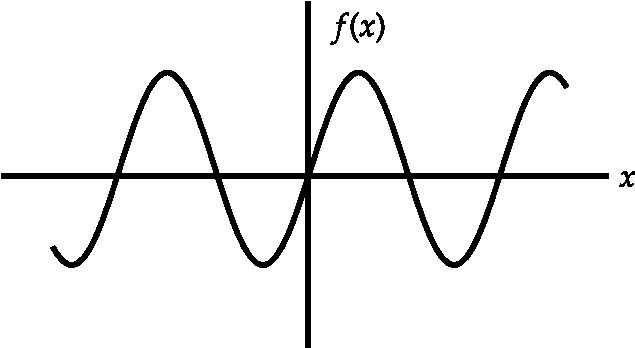
\includegraphics[height=3cm,width=5cm]{FT-Assignment-05}
	\end{figure}
	Which of the following graphs represents the real part of its Fourier transform?
	 \begin{tasks}(2)
		\task[\textbf{a.}]	
		\begin{figure}[H]
			\centering
			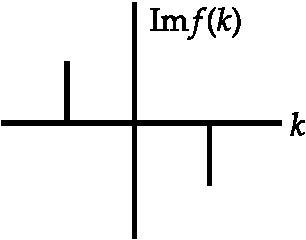
\includegraphics[height=2.2cm,width=3cm]{FT-Assignment-01}
		\end{figure}
		\task[\textbf{b.}]
			\begin{figure}[H]
			\centering
			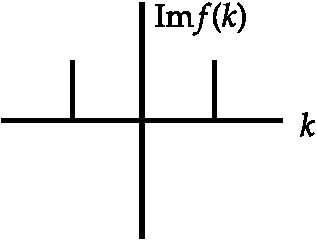
\includegraphics[height=2.2cm,width=3cm]{FT-Assignment-02}
		\end{figure}
		\task[\textbf{c.}]
			\begin{figure}[H]
			\centering
			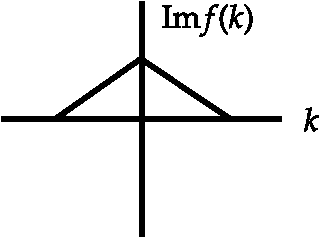
\includegraphics[height=2.2cm,width=3cm]{FT-Assignment-03}
		\end{figure}
		\task[\textbf{d.}] 
			\begin{figure}[H]
			\centering
			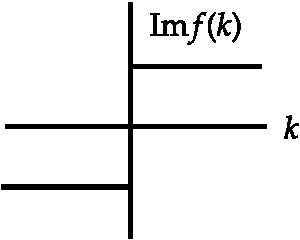
\includegraphics[height=2.2cm,width=3cm]{FT-Assignment-04}
		\end{figure}
	\end{tasks}
	\item The Fourier transform of the function $h(t)=\left\{\begin{array}{cc}\beta e^{-a t}, & t>0 \\ 0, & t<0\end{array}\right.$, is given by
	 \begin{tasks}(2)
		\task[\textbf{a.}]$H(f)=\frac{\alpha}{\sqrt{\alpha^{2}+(2 \pi f)^{2}}} e^{j \tan ^{-1}\left[-2 \pi f^{\prime \alpha]}\right.}$
		\task[\textbf{b.}]$H(f)=\frac{\beta}{\sqrt{\alpha^{2}+(2 \pi f)^{2}}} e^{j \tan ^{-1}[-2 \pi f / \beta]}$
		\task[\textbf{c.}]$H(f)=\frac{\beta}{\sqrt{\alpha^{2}+(2 \pi f)^{2}}} e^{\tan ^{-1}[2 \pi f / \alpha]}$
		\task[\textbf{d.}] $H(f)=\frac{\beta}{\sqrt{\alpha^{2}+(2 \pi f)^{2}}} e^{j \tan ^{-1}[-2 \pi f / \alpha]}$
	\end{tasks}
	\item The Fourier transform of $f(x)=\left\{\begin{array}{cl}-1 & -1<x<0 \\ 1 & 0<x<1 \\ 0 & \text { otherwise }\end{array}\right.$ is
	 \begin{tasks}(2)
		\task[\textbf{a.}] $\frac{i}{\omega} \sqrt{\frac{2}{\pi}}(\cos \omega+1)$
		\task[\textbf{b.}] $\frac{i}{\omega} \sqrt{\frac{2}{\pi}}(\cos \omega-1)$
		\task[\textbf{c.}]$-\frac{i}{\omega} \sqrt{\frac{2}{\pi}}(1+\cos \omega)$
		\task[\textbf{d.}] $\frac{i}{\omega} \sqrt{\frac{2}{\pi}}(1-\cos \omega)$
	\end{tasks}
	\item The Fourier transform of $f(x)= \begin{cases}x, & 0<x<a \\ 0, & \text { otherwise }\end{cases}$ is
	 \begin{tasks}(2)
		\task[\textbf{a.}]$\frac{1}{\sqrt{2 \pi} \cdot \omega^{2}}\left[e^{-i \omega n a}(1+i a \omega)-1\right]$
		\task[\textbf{b.}]$\frac{1}{\sqrt{2 \pi} \cdot \omega^{2}}\left[e^{-i \omega a}(1-i a \omega)-1\right]$
		\task[\textbf{c.}] $\frac{1}{\sqrt{2 \pi} \cdot \omega^{2}}\left[e^{-1 \text { tox }}(1+i a \omega)+1\right]$
		\task[\textbf{d.}] $\frac{1}{\sqrt{2 \pi} \cdot \omega^{2}}\left[e^{-i \omega a}(1-i a \omega)+1\right]$
	\end{tasks}
	
	
	
	
	
	
\end{enumerate}
%\chapter{Fourier Transform}
\begin{enumerate}
	\item  $\left. \right. $
	\begin{answer}
		\begin{align*}
		F(k)&=\frac{1}{\sqrt{2 \pi}} \int_{-\infty}^{+\infty} f(x) e^{i k x} d x\\
		\because g(x)&=f(x+a)\\
		\therefore G(k)&=\frac{1}{\sqrt{2 \pi}} \int_{-\infty}^{+\infty} f(x+a) e^{i k x} d x\\
		\text{Let }x+a&=y, d x=d y\\
		\therefore G(k)&=\frac{1}{\sqrt{2 \pi}} \int_{-\infty}^{+\infty} f(y) e^{i k(y-a)} d y=e^{-i k a} \frac{1}{\sqrt{2 \pi}} \int_{-\infty}^{+\infty} f(x) e^{i k x} d x=e^{-i a k} F(k)
	\end{align*}
		So the correct answer is \textbf{Option (c)}
	\end{answer}
	\item  $\left. \right. $
	\begin{answer}
		\begin{align*}
		 f_{c}(\omega) &=\sqrt{\frac{2}{\pi}} \int_{0}^{\infty} f(x) \cos \omega x d x \\ &=\sqrt{\frac{2}{\pi}} \int_{0}^{1} \cos \omega x d x+\sqrt{\frac{2}{\pi}} \int_{1}^{2}-\cos \omega x d x \\ &=\sqrt{\frac{2}{\pi}}\left[\left(\frac{\sin \omega x}{\omega}\right)_{0}^{1}-\left(\frac{\sin \omega x}{\omega}\right)_{1}^{2}\right] \\ &=\sqrt{\frac{2}{\pi}}\left(\frac{2 \sin \omega-\sin 2 \omega}{\omega}\right) 
		\end{align*}
		So the correct answer is \textbf{Option (b)}
	\end{answer}
	\item  $\left. \right. $
	\begin{answer}
		\begin{align*}
		\mathrm{n}: g(k)&=\frac{1}{\sqrt{2 \pi}} \int_{-\infty}^{+\infty} \frac{n}{\sqrt{\pi}} e^{-n^{2} x^{2}} e^{i k x} d x=\frac{n}{\sqrt{2} \cdot \pi} \int_{-\infty}^{+\infty} e^{-n^{2} x^{2}+i i x} d x=\frac{n}{\sqrt{2} \cdot \pi} e^{-k^{2} / 4 n^{2}} \int_{-\infty}^{+\infty} e^{-n^{2}\left(x-\frac{i k}{2 n^{2}}\right)^{2}} d x\\
		&=\frac{n}{\sqrt{2} \cdot \pi} e^{-k^{2} / 4 n^{2}} \times 2 \times \frac{1}{2} \cdot \frac{\sqrt{\pi}}{n}=\frac{1}{\sqrt{2 \pi}} e^{-k^{2} / 4 n^{2}}
		\intertext{ Now inverse fourier transform of $g(k)$ is}
		\delta_{n}(x)&=\frac{1}{\sqrt{2 \pi}} \int_{-\infty}^{+\infty} \frac{e^{-k^{2} / 4 n^{2}}}{\sqrt{2 \pi}} \cdot e^{-i k x} d k\\
		\delta(x)&=\lim _{n \rightarrow \infty} \delta_{n}(x)=\lim _{n \rightarrow \infty} \frac{1}{2 \pi} \int_{-\infty}^{+\infty} e^{-k^{2} / 4 n^{2}} \cdot e^{-i k x} d k=\frac{1}{2 \pi} \int_{-\infty}^{+\infty} e^{-i k x} d k\\
		\therefore \delta(x)&=\frac{1}{2 \pi} \int_{-\infty}^{+\infty} e^{-i k x} d k
		\end{align*}
		So the correct answer is \textbf{Option (c)}
	\end{answer}
	\item  $\left. \right. $	
	\begin{answer}
		\begin{align*}
		\text{(i) }g_{c}(\omega)=\sqrt{\frac{2}{\pi}} \int_{0}^{\omega} \delta(t-x) \cos \omega t d t=\sqrt{\frac{2}{\pi}} \cos \omega x
		\end{align*}
		So the correct answer is \textbf{Option (a)}
	\end{answer}
		\item  $\left. \right. $	
	\begin{answer}
		\begin{align*}
		f(t)&=\delta(t-x)=\sqrt{\frac{2}{\pi}} \int_{0}^{+\infty} \sqrt{\frac{2}{\pi}} \cos \omega x \cos \omega t d \omega\\
		\Rightarrow \delta(t-x)&=\frac{2}{\pi} \int_{0}^{\infty} \cos \omega t \cos \omega x d \omega
		\end{align*}
		So the correct answer is \textbf{Option (b)}
	\end{answer}
		\item  $\left. \right. $
	\begin{answer}
		\begin{align*}
		\intertext{Fourier Transform of $f(t)$ is}
		g(\omega)&=\frac{1}{\sqrt{2 \pi}} \int_{0}^{\infty} e^{-\Gamma t / 2 \hbar} \cdot e^{-i E_{0} / / \hbar} \cdot e^{i a t} d t=\frac{1}{\sqrt{2 \pi}} \int_{0}^{\infty} \exp \left\{\frac{-i t}{\hbar}\left(E_{0}-i \Gamma / 2-\hbar \omega\right)\right\} d t\\
		&=\frac{1}{\sqrt{2 \pi}}\left[\frac{e^{\left\{\frac{-i t}{\hbar}\left(E_{0}-i / / 2-\hbar \omega\right)\right\}}}{\frac{-i}{\hbar}\left(E_{0}-i \Gamma / 2-\hbar \omega\right)}\right]_{0}^{\infty}=\frac{1}{\sqrt{2 \pi}}\left[\frac{0-1}{\frac{-i}{\hbar}\left(E_{0}-i \Gamma / 2-\hbar \omega\right)}\right]\\
		&=\frac{1}{\sqrt{2 \pi} i(E o-i \Gamma / 2-h \omega)}
		\intertext{Inverse transform of $g(\omega)$ is}
		f(t)&=\frac{1}{2 \pi} \int_{-\infty}^{+\infty} \frac{\hbar e^{-i \omega x}}{i\left(E_{0}-i \Gamma / 2-\hbar \omega\right)} d \omega=\frac{\hbar}{2 \pi i} \int_{-\infty}^{+\infty} \frac{e^{-i \omega t} d \omega}{\left(E_{0}-i \Gamma / 2-\hbar \omega\right)}\\
		\therefore &\frac{\hbar}{2 \pi i} \int_{-\infty}^{+\infty} \frac{e^{-i \omega t} d \omega}{\left(E_{0}-i \Gamma / 2-\hbar \omega\right)}=f(t)= \begin{cases}\exp (-\Gamma t / 2 \hbar) \exp \left(\frac{-i E_{0} t}{\hbar}\right), & t>0 \\ 0 & t<0\end{cases}
		\end{align*}
		So the correct answer is \textbf{Option (c)}
	\end{answer}
	\item  $\left. \right. $
	\begin{answer}
		\begin{align*}
		F\left\{t e^{-r^{2}}\right\}&=-\frac{1}{2} F\left\{\frac{d\left(e^{-r^{2}}\right)}{d t}\right\}=-\frac{1}{2}(j 2 \pi f) F\left\{e^{-t^{2}}\right\}=-j \pi f e^{-\pi^{2} f^{2}}
		\end{align*}
		So the correct answer is \textbf{Option (b)}
	\end{answer}
		\item  $\left. \right. $
	\begin{answer}
		\begin{align*}
		\intertext{This is sine function}
		f(x)&=A \sin x \Rightarrow F(k)=j \frac{A}{2}\left[\delta\left(k-k_{0}\right)-\delta\left(k+k_{0}\right)\right]
		\end{align*}
		So the correct answer is \textbf{Option (a)}
	\end{answer}
		\item  $\left. \right. $
	\begin{answer}
		\begin{align*}
		H(f)&=\int_{-\infty}^{+\infty} h(t) e^{-j 2 \pi f t} d t=\int_{0}^{+\infty} \beta e^{-\alpha t} e^{-j 2 \pi f t} d t=\beta \int_{0}^{+\infty} e^{-(\alpha+j 2 \pi f) t} d t\\
		\Rightarrow H(f)&=\left.\frac{-\beta}{\alpha+j 2 \pi f} e^{-(\alpha+j 2 \pi f) t}\right|_{0} ^{\infty}=\frac{\beta}{\alpha+j 2 \pi f}=\frac{\beta \alpha}{\alpha^{2}+(2 \pi f)^{2}}-j \frac{2 \pi f \beta}{\alpha^{2}+(2 \pi f)^{2}}\\
		\Rightarrow H(f)&=\frac{\beta}{\sqrt{\alpha^{2}+(2 \pi f)^{2}}} e^{j \tan ^{-1}[-2 \pi f / \alpha]}
		\end{align*}
		So the correct answer is \textbf{Option (d)}
	\end{answer}
		\item  $\left. \right. $
	\begin{answer}
		\begin{align*}
		f(x)&=\left\{\begin{array}{rl}-1 & -1<x<0 \\ 1 & 0<x<1 \\ 0 & \text { otherwise }\end{array}\right.\\
		F[f(x)]&=\frac{1}{\sqrt{2 \pi}}\left[\int_{-1}^{0}-e^{-i \omega x} d x+\int_{0}^{1} e^{-i \omega x} d x\right]\\
		&=\frac{1}{\sqrt{2 \pi}}\left[-\left(\frac{e^{-i \omega x}}{-i \omega}\right)_{-1}^{0}+\left(\frac{e^{-i \omega x}}{-i \omega}\right)_{0}^{1}\right]=\frac{1}{\sqrt{2 \pi}}\left[\frac{-1+e^{i \omega}}{-i \omega}+\frac{e^{-i \omega}-1}{-i \omega}\right]\\
		&=\frac{1}{\sqrt{2 \pi}}\left[\frac{2 \cos \omega-2}{-i \omega}\right]=\frac{i}{\omega} \sqrt{\frac{2}{\pi}}(\cos \omega-1)
		\end{align*}
		So the correct answer is \textbf{Option (b)}
	\end{answer}
		\item  $\left. \right. $
		\begin{answer}
			\begin{align*}
			f(x)&= \begin{cases}x, & 0<x<a \\ 0, & \text { otherwise }\end{cases}\\
			F[f(x)]&=\frac{1}{\sqrt{2 \pi}} \int_{0}^{a} x e^{-i \omega x} d x=\frac{1}{\sqrt{2 \pi}}\left[\left(\frac{x e^{-i e x}}{-i \omega}\right)_{0}^{a}-\left(\frac{e^{-i \omega x}}{(-i \omega)^{2}}\right)_{0}^{a}\right]\\&=\frac{1}{\sqrt{2 \pi}}\left[\frac{a e^{-i \omega a}}{-i \omega}-\frac{e^{-i \omega a}-1}{(-i \omega)^{2}}\right]=\frac{1}{\sqrt{2 \pi}}\left[\frac{i a \omega e^{-i e a}}{\omega^{2}}+\frac{e^{-i e a}-1}{\omega^{2}}\right]\\
			&=\frac{1}{\sqrt{2 \pi} \cdot \omega^{2}}\left[e^{-i \omega x}(1+i a \omega)-1\right]
			\end{align*}
			So the correct answer is \textbf{Option (a)}
		\end{answer}
\end{enumerate}
%\chapter{Complex Problem Set}
\begin{abox}
	Practise Set-1
\end{abox}
\begin{enumerate}[label=\color{ocre}\textbf{\arabic*.}]
	\item The value of the integral $\int_{C} d z z^{2} e^{z}$, where $C$ is an open contour in the complex $z$-plane as shown in the figure below, is:
	{\exyear{NET/JRF(JUNE-2011)}}
	\begin{figure}[H]
		\centering
		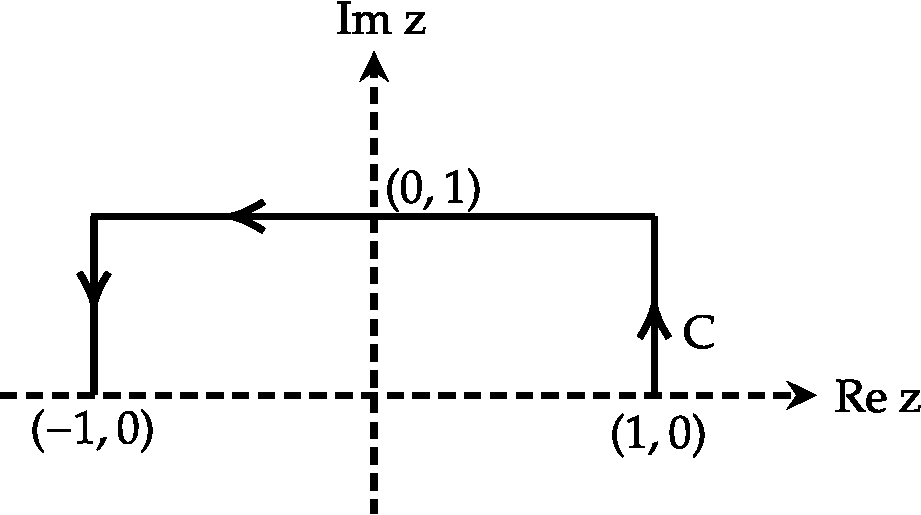
\includegraphics[height=5cm,width=9cm]{diagram-20211005-crop}
	\end{figure}
	\begin{tasks}(4)
		\task[\textbf{A.}] $\frac{5}{e}+e$
		\task[\textbf{B.}] $e-\frac{5}{e}$
		\task[\textbf{C.}] $\frac{5}{e}-e$
		\task[\textbf{D.}] $-\frac{5}{e}-e$
	\end{tasks}
	\begin{answer}
		\begin{align*}
		\intertext { If we complete the contour, then by Cauchy integral theorem }
		\int_{-1}^{1} d z z^{2} e^{z}+\int_{C} d z z^{2} e^{z}&=0 \Rightarrow \int_{C} d z z^{2} e^{z}=-\int_{-1}^{1} d z z^{2} e^{z}\\&=-\left[z^{2} e^{z}-2 z e^{2}+2 e^{2}\right]_{-1}^{1}=\frac{5}{e}-e
		\end{align*}
		So the correct answer is \textbf{Option (C)}
	\end{answer}
	\item Which of the following is an analytic function of the complex variable $z=x+i y$ in the domain $|z|<2 ?$
	{\exyear{NET/JRF(JUNE-2011)}}
	\begin{tasks}(2)
		\task[\textbf{A.}] $(3+x-i y)^{7}$
		\task[\textbf{B.}] $(1+x+i y)^{4}(7-x-i y)^{3}$
		\task[\textbf{C.}] $(1-x-i y)^{4}(7-x+i y)^{3}$
		\task[\textbf{D.}] $(x+i y-1)^{1 / 2}$
	\end{tasks}
	\begin{answer}
		Put $z=x+i y .$ If $\bar{z}=x-i y$ appears in any of the expressions then that expression is non-analytic. For option (D) we have a branch point singularity as the power is $\frac{1}{2}$ which is fractional. Hence only option (B) is analytic.\\\\
		So the correct answer is \textbf{Option (B)}
	\end{answer}
	\item The first few terms in the Laurent series for $\frac{1}{(z-1)(z-2)}$ in the region $1 \leq|z| \leq 2$ and around $z=1$ is
	{\exyear{NET/JRF(JUNE-2012)}}
	\begin{tasks}(1)
		\task[\textbf{A.}] $\frac{1}{2}\left[1+z+z^{2}+\ldots\right]\left[1+\frac{z}{2}+\frac{z^{2}}{4}+\frac{z^{3}}{8}+\ldots .\right]$
		\task[\textbf{B.}] $\frac{1}{1-z}-z-(1-z)^{2}+(1-z)^{3}+\ldots .$
		\task[\textbf{C.}] $\frac{1}{\mathrm{z}^{2}}\left[1+\frac{1}{\mathrm{z}}+\frac{1}{\mathrm{z}^{2}}+\ldots .\right]\left[1+\frac{2}{\mathrm{z}}+\frac{4}{\mathrm{z}^{2}}+\ldots . .\right]$
		\task[\textbf{D.}]  $2(z-1)+5(z-1)^{2}+7(z-1)^{3}+\ldots$
	\end{tasks}
	\begin{answer}
		\begin{align*}
		\frac{1}{(z-1)(z-2)}&=\frac{1}{z-2}-\frac{1}{z-1}=\frac{1}{1-z}+\frac{1}{(z-1)-1}\\&=\frac{1}{1-z}-(1+(1-z))^{-1}\\
		&=\frac{1}{1-z}-\left[1+(1-z)+\frac{(-1)(-2)}{2 !}(1-z)^{2}+\frac{(-1)(-2)(-3)}{3 !}(1-z)^{3} \ldots\right]\\
		&=\frac{1}{1-z}-\left[z+(1-z)^{2}-(1-z)^{3}+\ldots . .\right]
		\end{align*}
		So the correct answer is \textbf{Option (B)}
	\end{answer}
	\item Let $u(x, y)=x+\frac{1}{2}\left(x^{2}-y^{2}\right)$ be the real part of analytic function $f(z)$ of the complex variable $z=x+i y$. The imaginary part of $f(z)$ is
	{\exyear{NET/JRF(JUNE-2012)}}
	\begin{tasks}(4)
		\task[\textbf{A.}] $y+x y$
		\task[\textbf{B.}] $x y$
		\task[\textbf{C.}] $y$
		\task[\textbf{D.}] $y^{2}-x^{2}$
	\end{tasks}
	\begin{answer}
		\begin{align*}
		u(x, y)&=x+\frac{1}{2}\left(x^{2}-y^{2}\right), v(x, y)=?\\
		\text{Check }\frac{\partial u}{\partial x}&=\frac{\partial v}{\partial y}\text{ and } \frac{\partial u}{\partial y}=-\frac{\partial v}{\partial x}\\
		\Rightarrow \frac{\partial u}{\partial x}&=\frac{\partial v}{\partial y}, \quad \frac{\partial v}{\partial y}=1+x, \\ v&=y+x y+f(x)\\
		\frac{\partial u}{\partial y}&=-\frac{\partial v}{\partial x} \Rightarrow \frac{\partial v}{\partial x}=+y, \\ v&=y x+f(y)\\
		y+x y+f(x)&=y x+f(y)\\
		\text{If }f(x)&=0\quad \quad
		f(y)=y\\
		v&=x y+y
		\end{align*}
		So the correct answer is \textbf{Option (A)}
	\end{answer}
	\item The value of the integral $\int_{C} \frac{z^{3} d z}{\left(z^{2}-5 z+6\right)}$, where $C$ is a closed contour defined by the equation $2|z|-5=0$, traversed in the anti-clockwise direction, is
	{\exyear{NET/JRF(DEC-2012)}}
	\begin{tasks}(4)
		\task[\textbf{A.}] $-16 \pi i$
		\task[\textbf{B.}] $16 \pi \mathrm{i}$
		\task[\textbf{C.}] $8 \pi i$
		\task[\textbf{D.}] $2 \pi i$
	\end{tasks}
	\begin{answer}
		\begin{align*}
		z^{2}-5 z+6&=0 \Rightarrow z^{2}-2 z-3 z+6\\&=0 \Rightarrow z(z-2)-3(z-2)=0 \Rightarrow z=3,2\\
		2|z|&=5 \Rightarrow|z|=2.5,\text{ only 2 will be inside.}\\
		\text{Residue }&=\left.(z-2) \frac{z^{3}}{(z-3)(z-2)}\right|_{z=2}=\frac{8}{2-3}\\&=-8 \Rightarrow \int \frac{z^{3} d z}{z^{2}-5 z+6}=2 \pi i(-8)=-16 \pi i
		\end{align*}
		So the correct answer is \textbf{Option (A)}
	\end{answer}
	\item  With $z=x+i y$, which of the following functions $f(x, y)$ is NOT a (complex) analytic function of $z$ ?
	{\exyear{NET/JRF(JUNE-2013)}}
	\begin{tasks}(1)
		\task[\textbf{A.}] $f(x, y)=(x+i y-8)^{3}\left(4+x^{2}-y^{2}+2 i x y\right)^{7}$
		\task[\textbf{B.}] $f(x, y)=(x+i y)^{7}(1-x-i y)^{3}$
		\task[\textbf{C.}] $f(x, y)=\left(x^{2}-y^{2}+2 i x y-3\right)^{5}$
		\task[\textbf{D.}] $f(x, y)=(1-x+i y)^{4}(2+x+i y)^{6}$
	\end{tasks}
	\begin{answer}
		\begin{align*}
		f(x, y)&=(1-x+i y)^{4}(2+x+i y)^{6}\\&=\{1-(x-i y)\}^{4}(2+x+i y)^{6}\\
		\text{Due to present of }\bar{z}&=(x-i y)
		\end{align*}
		So the correct answer is \textbf{Option (D)}
	\end{answer}
	\item  Which of the following functions cannot be the real part of a complex analytic function of $z=x+i y ?$
	{\exyear{NET/JRF(DEC-2013)}}
	\begin{tasks}(4)
		\task[\textbf{A.}] $x^{2} y$
		\task[\textbf{B.}]  $x^{2}-y^{2}$
		\task[\textbf{C.}] $x^{3}-3 x y^{2}$
		\task[\textbf{D.}] $3 x^{2} y-y-y^{3}$
	\end{tasks}
	\begin{answer}
		\begin{align*}
		\intertext{ Let $x^{2} y$ be real part of a complex function. Use Milne Thomson's method to write analytic complex function. The real part of that function should be (1) but that is not the case. So this cannot be real part of an analytic function. Also,}
		z^{2}&=(x+i y)^{2}=x^{2}-y^{2}+2 i x y,\text{ Real part option (2)}\\
		z^{3}&=(x+i y)^{3}=x^{3}-i y^{3}+3 i x y(x+i y)\\
		&=x^{3}-i y^{3}+3 i x^{2} y-3 x y^{2},\text{ Real part option (3)}
		\end{align*}
		So the correct answer is \textbf{Option (A)}
	\end{answer}
	\item  Given that the integral $\int_{0}^{\infty} \frac{d x}{y^{2}+x^{2}}=\frac{\pi}{2 y}$, the value of $\int_{0}^{\infty} \frac{d x}{\left(y^{2}+x^{2}\right)^{2}}$ is
	{\exyear{NET/JRF(DEC-2013)}}
	\begin{tasks}(4)
		\task[\textbf{A.}] $\frac{\pi}{y^{3}}$
		\task[\textbf{B.}] $\frac{\pi}{4 y^{3}}$
		\task[\textbf{C.}]  $\frac{\pi}{8 y^{3}}$
		\task[\textbf{D.}] $\frac{\pi}{2 y^{3}}$
	\end{tasks}
	\begin{answer}
		\begin{align*}
		\int_{0}^{\infty} \frac{d x}{\left(y^{2}+x^{2}\right)^{2}}&=\frac{1}{2} \int_{-\infty}^{\infty} \frac{d x}{\left(y^{2}+x^{2}\right)^{2}},\text{ pole is of }2^{\text {nd }}\text{ order at }x=i y,\text{ residue }=1 /\left(4 i y^{3}\right)\\
		\text{Integral }&=\left(\frac{1}{2}\right)(2 \pi i) \frac{1}{4 i y^{3}}=\frac{\pi}{\left(4 y^{3}\right)}
		\end{align*}
	\end{answer}
	\item If $C$ is the contour defined by $|z|=\frac{1}{2}$, the value of the integral
	$$
	\oint_{C} \frac{d z}{\sin ^{2} z}
	$$
	is
	{\exyear{NET/JRF(JUNE-2014)}}
	\begin{tasks}(4)
		\task[\textbf{A.}] $\infty$
		\task[\textbf{B.}] $2 \pi i$
		\task[\textbf{C.}] 0
		\task[\textbf{D.}] $\pi i$
	\end{tasks}
	\begin{answer}
		\begin{align*}
		f(z)&=\frac{1}{\sin ^{2} z} \quad\left(|z|=\frac{1}{2}\right)\\
		\sin z&=z-\frac{z^{3}}{\lfloor 3}+\frac{z^{5}}{\lfloor 5} \ldots . \Rightarrow \frac{1}{\sin ^{2} z}=\frac{1}{\left(z-\frac{z^{3}}{\frac{3}{3}}+\frac{z^{5}}{5} \cdots\right)^{2}}\\
		\Rightarrow \frac{1}{\sin ^{2} z}&=\frac{1}{z^{2}}\left[1-\frac{z^{2}}{\lfloor 3}+\frac{z^{4}}{\lfloor 5} \ldots .\right]^{-2} \Rightarrow \oint_{C} \frac{d z}{\sin ^{2} z}=0
		\end{align*}
		So the correct answer is \textbf{Option (C)}
	\end{answer}
	\item The principal value of the integral $\int_{-\infty}^{\infty} \frac{\sin (2 x)}{x^{3}} d x$ is
	{\exyear{NET/JRF(DEC-2014)}}
	\begin{tasks}(4)
		\task[\textbf{A.}] $-2 \pi$
		\task[\textbf{B.}]  $-\pi$
		\task[\textbf{C.}] $\pi$
		\task[\textbf{D.}]  $2 \pi$
	\end{tasks}
	\begin{answer}
		\begin{align*}
		\text{Let }f(z)&=\frac{e^{i 2 z}}{z^{3}}\\
		\lim _{2 \rightarrow 0}(z-0)^{3} f(z)&=\lim _{z \rightarrow 0}(z-0)^{3} \frac{e^{i 2 z}}{z^{3}}\\&=1(\text{ finite and }\neq 0) \Rightarrow z=0 \text{is pole of order 3} .\\
		\text{Residue }R&=\frac{1}{2 !} \lim _{z \rightarrow 0} \frac{d^{2}}{d z^{2}}\left[(z-0)^{3} \frac{e^{i 2 z}}{z^{3}}\right]=-2\\
		\Rightarrow \int_{-\infty}^{\infty} f(x) d x&=\pi i \Sigma R=\pi i(-2)=-2 \pi i \Rightarrow \operatorname{Im} .\text{ Part }\\&=-2 \pi \Rightarrow \int_{-\infty}^{\infty} f(x) d x=-2 \pi
		\end{align*}
		So the correct answer is \textbf{Option (A)}
	\end{answer}
	\item The Laurent series expansion of the function $f(z)=e^{2}+e^{1 / 2}$ about $z=0$ is given by
	{\exyear{NET/JRF(DEC-2014)}}
	\begin{tasks}(2)
		\task[\textbf{A.}] $\sum_{n=-\infty}^{\infty} \frac{z^{n}}{n !}$ for all $|z|<\infty$
		\task[\textbf{B.}] $\sum_{n=0}^{\infty}\left(z^{n}+\frac{1}{z^{n}}\right) \frac{1}{n !}$ only if $0<|z|<1$
		\task[\textbf{C.}] $\sum_{n=0}^{\infty}\left(z^{n}+\frac{1}{z^{n}}\right) \frac{1}{n !}$ for all $0<|z|<\infty$
		\task[\textbf{D.}]  $\sum_{n=-\infty}^{\infty} \frac{z^{n}}{n !}$ only if $|z|<1$
	\end{tasks}
	\begin{answer}
		\begin{align*}
		e^{z}&=\left(1+z+\frac{z^{2}}{2 !}+\ldots\right)=\sum_{n=0}^{\infty} \frac{z^{n}}{n !}\text{ and }e^{1 / z}\\&=1+\frac{1}{z}+\frac{1}{2 !} \frac{1}{z^{2}}+\ldots .=\sum_{n=0}^{\infty} \frac{1}{z^{n} n !}\\
		\Rightarrow f(z)&=\left(e^{z}+e^{1 / 2}\right)=\sum_{n=0}^{\infty}\left(z^{n}+\frac{1}{z^{n}}\right) \frac{1}{n !},\text{ for all }0<|z|<\infty
		\end{align*}
		So the correct answer is \textbf{Option (C)}
	\end{answer}
	\item Consider the function $f(z)=\frac{1}{z} \ln (1-z)$ of a complex variable $z=r e^{i \theta}(r \geq 0, \quad-\infty<\theta<\infty)$. The singularities of $f(z)$ are as follows:
	{\exyear{NET/JRF(DEC-2014)}}
	\begin{tasks}(1)
		\task[\textbf{A.}]  Branch points at $z=1$ and $z=\infty$; and a pole at $z=0$ only for $0 \leq \theta<2 \pi$
		\task[\textbf{B.}] Branch points at $z=1$ and $z=\infty$; and a pole at $z=0$ for all $\theta$ other than $0 \leq \theta<2 \pi$
		\task[\textbf{C.}] Branch points at $z=1$ and $z=\infty$; and a pole at $z=0$ for all $\theta$
		\task[\textbf{D.}] Branch points at $z=0, z=1$ and $z=\infty$.
	\end{tasks}
	\begin{answer}
		\begin{align*}
		\text{For }f(z)&=\frac{1}{z} \ln (1-z)=\frac{1}{z}\left(-z-\frac{z^{2}}{2}-\frac{z^{3}}{3}-\ldots . .\right)\\&=-1-\frac{z}{2}-\frac{z^{2}}{3}-\ldots .
		\intertext{There is no principal part and when $z \rightarrow 0, f(z)=-1 .$ So there is removable singularity at $z=0$. Also $z=1$ and $z=\infty$ is Branch point.}
		\end{align*}
		None of the above is correct
	\end{answer}
	\item  The value of integral $\int_{-\infty}^{\infty} \frac{d x}{1+x^{4}}$
	{\exyear{NET/JRF(JUNE-2015)}}
	\begin{tasks}(4)
		\task[\textbf{A.}] $\frac{\pi}{\sqrt{2}}$
		\task[\textbf{B.}] $\frac{\pi}{2}$
		\task[\textbf{C.}] $\sqrt{2} \pi$
		\task[\textbf{D.}] $2 \pi$
	\end{tasks}
	\begin{answer}
		\begin{align*}
		\int_{-\infty}^{\infty} \frac{d z}{1+z^{4}} \quad \because|z|=R\\
		\text{Now, pole }z&=e^{(2 n+1) \frac{\pi}{4}}\\
		n&=0, \quad \Rightarrow z_{0}=e^{\frac{i \pi}{4}}=\frac{1}{\sqrt{2}}+i \frac{1}{\sqrt{2}}, n\\&=2 \Rightarrow z_{2}=\frac{-1}{\sqrt{2}}-i \frac{1}{\sqrt{2}}\\
		n&=1 \Rightarrow z_{1}=e^{\frac{i 3 \pi}{4}}=\frac{-1}{\sqrt{2}}+i \frac{1}{\sqrt{2}}, n\\&=3 \Rightarrow z_{3}=+\frac{1}{\sqrt{2}}-i \frac{1}{\sqrt{2}}
		\intertext{only $z_{0}$ and $z_{1}$ lies in contour}
		\text{i.e., residue at }\left(z=e^{\frac{i \pi}{4}}\right)&=\frac{1}{4}\left(-\frac{1}{\sqrt{2}}-i \frac{1}{\sqrt{2}}\right)\\
		\text{residue at }\left(z=e^{\frac{i 3 \pi}{4}}\right)&=\frac{1}{4}\left(\frac{1}{\sqrt{2}}-i \frac{1}{\sqrt{2}}\right)\\
		\text{now }\int_{-\infty}^{\infty} \frac{d x}{x^{4}+1}&=2 \pi i \Sigma \operatorname{Re} S=\frac{\pi}{\sqrt{2}}
		\end{align*}
		So the correct answer is \textbf{Option (A)}
	\end{answer}
	\item  The function $\frac{Z}{\sin \pi z^{2}}$ of a complex variable $z$ has
	{\exyear{NET/JRF(DEC-2015)}}
	\begin{tasks}(1)
		\task[\textbf{A.}] A simple pole at 0 and poles of order 2 at $\pm \sqrt{n}$ for $n=1,2,3 \ldots$
		\task[\textbf{B.}] A simple pole at 0 and poles of order 2 at $\pm \sqrt{n}$ and $\pm i \sqrt{n}$ for $n=1,2,3 \ldots$
		\task[\textbf{C.}] Poles of order 2 at $\pm \sqrt{n}, n=0,1,2,3 \ldots$
		\task[\textbf{D.}] Poles of order 2 at $\pm n, n=0,1,2,3 \ldots$
	\end{tasks}
	\begin{answer}
		\begin{align*}
		f(z)&=\frac{z}{\sin \pi z^{2}}=\frac{z}{\pi z^{2} \frac{\sin \pi z^{2}}{\pi z^{2}}}\\
		\text{	at }z&=0,\text{ it is a simple pole since,} \lim _{z \rightarrow 0} \frac{\sin \pi z^{2}}{\pi z^{2}}=1\\
		\text{Also, }\sin \pi z^{2}&=\sin n \pi \Rightarrow \pi \mathrm{z}^{2}\\&=\pm n \pi, z=\pm \sqrt{n}, \pm i \sqrt{n}\\
		\lim _{z \rightarrow \sqrt{n}}&(z-\sqrt{n})^{2} \cdot \frac{z}{\sin \pi z^{2}}, \text{exists. So its pole of order 2}
		\end{align*}
		So the correct answer is \textbf{Option (B)}
	\end{answer}
	\item The value of the contour integral $\frac{1}{2 \pi i} \oint_{C} \frac{e^{4 z}-1}{\cosh (z)-2 \sinh (z)} d z$ around the unit circle $C$ traversed in the anti-clockwise direction, is
	{\exyear{NET/JRF(JUNE-2016)}}
	\begin{tasks}(4)
		\task[\textbf{A.}] 0
		\task[\textbf{B.}] 2
		\task[\textbf{C.}] $\frac{-8}{\sqrt{3}}$
		\task[\textbf{D.}] $-\tanh \left(\frac{1}{2}\right)$
	\end{tasks}
	\begin{answer}
		\begin{align*}
		f(z)&=\frac{e^{4 z}-1}{\cosh z-2 \sinh z}=\frac{e^{4 z}-1}{\frac{e^{2}+e^{-z}}{2}-\left(e^{z}-e^{-z}\right)}\\&=\frac{e^{42}-1}{-\frac{e^{z}}{2}+\frac{3}{2} e^{-z}}\\
		\Rightarrow f(z)&=\frac{2 e^{2}\left(e^{4 z}-1\right)}{\left(3-e^{2 z}\right)}=\frac{2\left(e^{5 z}-e^{z}\right)}{\left(3-e^{2 z}\right)}\\
		\text{For pole at }z&=z_{0}, 3-e^{2 \xi_{0}}=0 \Rightarrow e^{2 z_{0}}\\&=3 \Rightarrow z_{0}=\frac{\ln 3}{2}
		\intertext{It has simple pole at $z_{0}$}
		\operatorname{Re}\left(z_{0}\right)&=\lim _{z \rightarrow z_{0}}\left(z-z_{0}\right) f(z)=\lim _{2 \rightarrow z_{0}}\left(z-z_{0}\right) \frac{2\left(e^{5 z}-e^{2}\right)}{3-e^{22}}\\
		&=\lim _{z \rightarrow z_{0}} \frac{\left(z-z_{0}\right) \times 2\left(5 e^{5 z}-e^{z}\right)+2\left(e^{5 z}-e^{z}\right) \times 1}{-2 e^{2 z}}\\&=-\left(\frac{e^{5 z_{0}}-e^{z_{0}}}{e^{2 z_{0}}}\right)\\
		&=-\left(\frac{(\sqrt{3})^{5}-\sqrt{3}}{3}\right)=-\left(\frac{9 \sqrt{3}-\sqrt{3}}{3}\right)=-\frac{8}{\sqrt{3}}\\
		\frac{1}{2 \pi i} \oint f(z) d z&=\frac{1}{2 \pi i} \times 2 \pi i \sum\text{ Residue } =-\frac{8}{\sqrt{3}}
		\end{align*}
		So the correct answer is \textbf{Option (C)}
	\end{answer}
	\item  Let $u(x, y)=e^{a x} \cos (b y)$ be the real part of a function $f(z)=u(x, y)+i v(x, y)$ of the complex variable $z=x+i y$, where $a, b$ are real constants and $a \neq 0 .$ The function $f(z)$ is complex analytic everywhere in the complex plane if and only if
	{\exyear{NET/JRF(JUNE-2017)}}
	\begin{tasks}(4)
		\task[\textbf{A.}] $b=0$
		\task[\textbf{B.}] $b=\pm a$
		\task[\textbf{C.}] $b=\pm 2 \pi a$
		\task[\textbf{D.}]  $b=a \pm 2 \pi$
	\end{tasks}
	\begin{answer}
		\begin{align*}
		\intertext{The function $f(z)$ will be analytic everywhere in the complex plane if and only if it satisfies the Cauchy Riemann equation in that region.}
		\Rightarrow \frac{\partial u}{\partial x}&=\frac{\partial v}{\partial y}\text{ and } \frac{\partial u}{\partial y}=-\frac{\partial v}{\partial x}\\
		\text{Hence }a e^{a x} \cos (b y)&=\frac{\partial v}{\partial y}\hspace{2cm}\text{(i)}\\
		\text{and }b e^{a x} \sin (b y)&=\frac{\partial v}{\partial x}\hspace{2cm}\text{(ii)}
		\intertext{From equation (i)}
		v(x, y)&=\frac{a e^{a x} \sin (b y)}{b}+c(y)\hspace{2cm}\text{(iii)}
		\intertext{Differentiating partially with $x$ gives}
		\frac{\partial v}{\partial x}&=\frac{a^{2} e^{a x} \sin (b y)}{b}\hspace{2cm}\text{(iv)}
		\intertext{From equation (iii) and (iv)}
		b e^{a x} \sin (b y)&=\frac{a^{2} e^{a x} \sin (b y)}{b}\\
		\Rightarrow b^{2}&=a^{2} \Rightarrow b=\pm a
		\end{align*}
		So the correct answer is \textbf{Option (B)}
	\end{answer}
	\item  The integral $\oint_{\Gamma} \frac{z e^{i \pi z / 2}}{z^{2}-1} d z$ along the closed contour $\Gamma$ shown in the figure is
	{\exyear{NET/JRF(JUNE-2017)}}
	\begin{figure}[H]
		\centering
		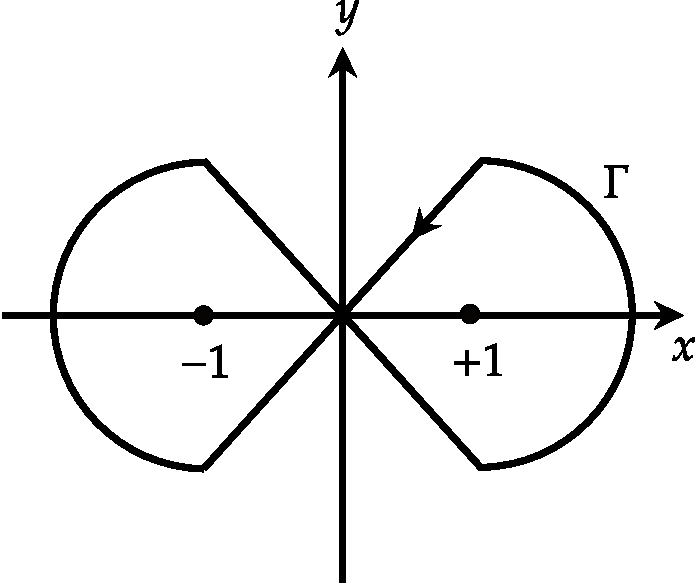
\includegraphics[height=4cm,width=5cm]{diagram-20211005(19)-crop}
	\end{figure}
	\begin{tasks}(4)
		\task[\textbf{A.}] 0
		\task[\textbf{B.}] $2 \pi$
		\task[\textbf{C.}] $-2 \pi$
		\task[\textbf{D.}] $4 \pi i$
	\end{tasks}
	\begin{answer}
		\begin{align*}
		f(z)&=\frac{z e^{i z \pi / 2}}{(z+1)(z-1)}\\
		\text{For }z&=+1\text{ anti-clockwise}\\
		I&=2 \pi i \lim _{z \rightarrow 1} \frac{z e^{i \pi z / 2}}{(z+1)}=\frac{2 \pi i}{2} e^{i \pi / 2}=\pi i e^{i \pi / 2}\\
		\text{For }z&=-1\\
		I&=-2 \pi i \lim _{z \rightarrow-1} \frac{z e^{i \pi z / 2}}{(z-1)}=-2 \pi i \times \frac{(-1) e^{-i \pi / 2}}{(-2)}=-\pi i e^{-i \pi / 2}\\
		\text{Integral }&=\pi i \frac{\left(e^{i \pi / 2}-e^{-i \pi / 2}\right)}{2 i} \times 2 i=2 \pi i^{2} \sin \frac{\pi}{2}=-2 \pi
		\end{align*}
		So the correct answer is \textbf{Option (C)}
	\end{answer}
	\item What is the value of $a$ for which $f(x, y)=2 x+3\left(x^{2}-y^{2}\right)+2 i(3 x y+a y)$ is an analytic function of complex variable $z=x+i y$
	{\exyear{NET/JRF(JUNE-2018)}}
	\begin{tasks}(4)
		\task[\textbf{A.}] 1
		\task[\textbf{B.}] 0
		\task[\textbf{C.}] 3
		\task[\textbf{D.}] 2
	\end{tasks}
	\begin{answer}
		\begin{align*}
		f(x, y)&=2 x+3\left(x^{2}-y^{2}\right)+2 i(3 x y+\alpha y)\\
		u&=2 x+3\left(x^{2}-y^{2}\right), v=2(3 x y+\alpha y)\\
		\text{C-R conditions: }u_{x}&=v_{y}, u_{y}=-v_{x}\\
		2+3(2 x)&=2(3 x+\alpha) \Rightarrow \alpha=1 \Rightarrow-6 y=-6 y
		\end{align*}
		So the correct answer is \textbf{Option (A)}
	\end{answer}
	\item  The value of the integral $\oint_{C} \frac{d z}{z} \frac{\tanh 2 z}{\sin \pi z}$, where $C$ is a circle of radius $\frac{\pi}{2}$, traversed counter-clockwise, with centre at $z=0$, is
	{\exyear{NET/JRF(DEC-2018)}}
	\begin{tasks}(4)
		\task[\textbf{A.}] 4
		\task[\textbf{B.}] $4 i$
		\task[\textbf{C.}] $2 i$
		\task[\textbf{D.}] 0
	\end{tasks}
	\begin{answer}$\left. \right. $
		\begin{figure}[H]
			\centering
			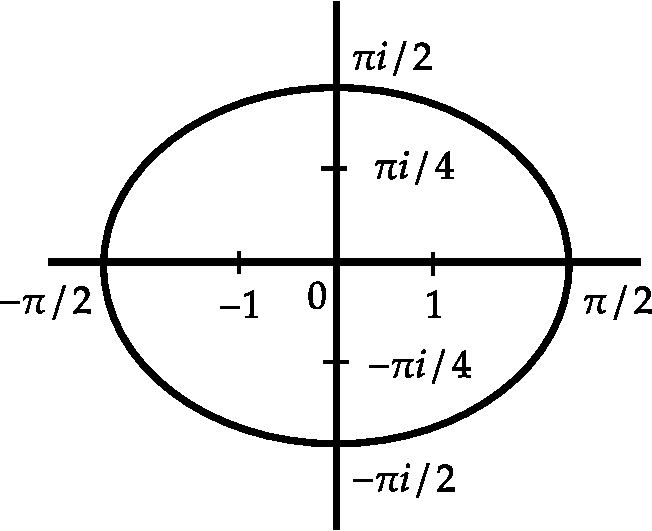
\includegraphics[height=4.5cm,width=5.5cm]{diagram-20211005(2)-crop}
		\end{figure}
		\begin{align*}
		&\oint_{C} \frac{d z}{z} \frac{\tanh 2 z}{\sin \pi z} d z\\
		z&=0,1,-1, \frac{\pi i}{4}, \frac{-\pi i}{4}\\
		f(z)&=\frac{2 z-\frac{1}{3}(2 z)^{3}+\frac{2}{15}(2 z)^{5} \ldots .}{z\left(\pi z-\frac{\pi^{3} z^{3}}{3 !}+\ldots\right)}\\
		\frac{2}{\pi z}&\left(1-\frac{1}{2} z^{2}+\ldots\right)\left(1-\frac{\pi^{2} z^{2}}{2 !}+\ldots\right)\\
		b_{1}&=\frac{2}{\pi}\\
		\text{As Re } z&=1, \frac{\tanh ^{2}}{-\pi}\text{ and }\operatorname{Re} z=-1, \frac{\tanh ^{2}}{-\pi}\\
		\operatorname{Re} z&=\frac{i \pi}{4}=-\frac{1}{\pi}\left(2 \operatorname{cosec} h \frac{\pi^{2}}{4}\right)\\
		\operatorname{Re} z&=\frac{-i \pi}{4}=-\frac{1}{\pi}\left(2 \operatorname{cosec} \mathrm{h} \frac{\pi^{2}}{4}\right)
		\intertext{$I=2 \pi i \Sigma R=4 i$ only when 0 lies inside, otherwise wrong question.}
		\end{align*}
		So the correct answer is \textbf{Option (B)}
	\end{answer}
	\item The integral $I=\int_{C} e^{z} d z$ is evaluated from the point $(-1,0)$ to $(1,0)$ along the contour $C$, which is an arc of the parabola $y=x^{2}-1$, as shown in the figure. The value of $I$ is
	{\exyear{NET/JRF(DEC-2018)}}
	\begin{figure}[H]
		\centering
		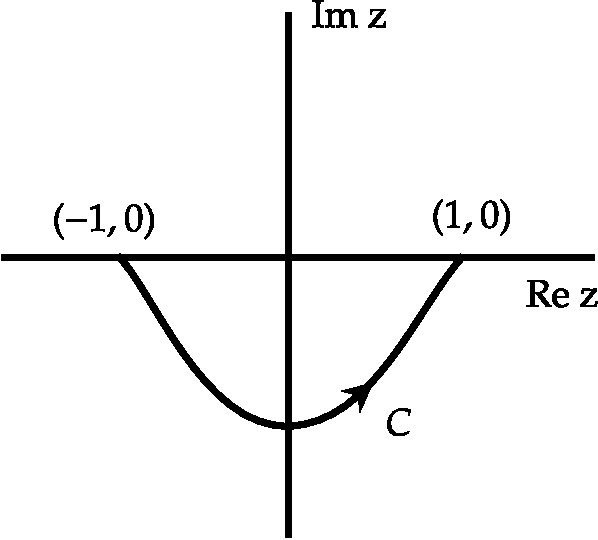
\includegraphics[height=4.5cm,width=5cm]{diagram-20211005(3)-crop}
	\end{figure}
	\begin{tasks}(4)
		\task[\textbf{A.}]  0
		\task[\textbf{B.}] $2 \sinh 1$
		\task[\textbf{C.}]  $e^{2 i} \sinh 1$
		\task[\textbf{D.}] $e+e^{-1}$
	\end{tasks}
	\begin{answer}
		\begin{align*}
		\int_{C} f(z) d z&=2 \pi i \Sigma R\\
		\int_{C} f(z) d z+\int_{1}^{-1} e^{x} d x&=0\\
		\int_{C} f(z) d z&=-\int_{1}^{-1} e^{x} d x=\int_{1}^{-1} e^{x} d x\\&=\frac{\left(e^{1}-e^{-1}\right)}{2} \cdot 2=2 \sinh 1
		\end{align*}
		So the correct answer is \textbf{Option (B)}
	\end{answer}
	\item The contour $C$ of the following integral
	$$
	\oint_{C} d z \frac{\sqrt{(z-1)(z-3)}}{\left(z^{2}-25\right)^{3}}
	$$
	in the complex $z$ plane is shown in the figure below.\\
	\begin{figure}[H]
		\centering
		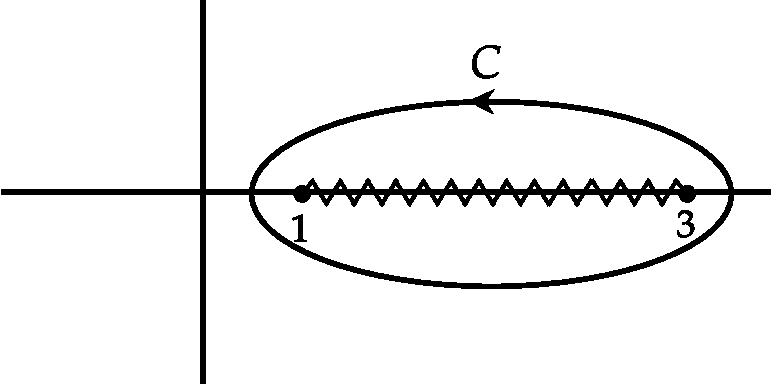
\includegraphics[height=3.5cm,width=6cm]{diagram-20211005(8)-crop}
	\end{figure}
	This integral is equivalent to an integral along the contours
	{\exyear{NET/JRF(DEC-2018)}}
	\begin{tasks}(2)
		\task[\textbf{A.}] \begin{figure}[H]
			\centering
			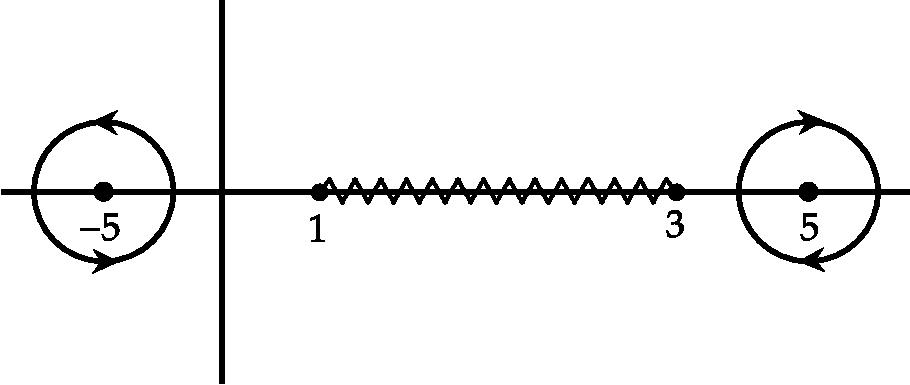
\includegraphics[height=3cm,width=6.5cm]{diagram-20211005(4)-crop}
		\end{figure}
		\task[\textbf{B.}] \begin{figure}[H]
			\centering
			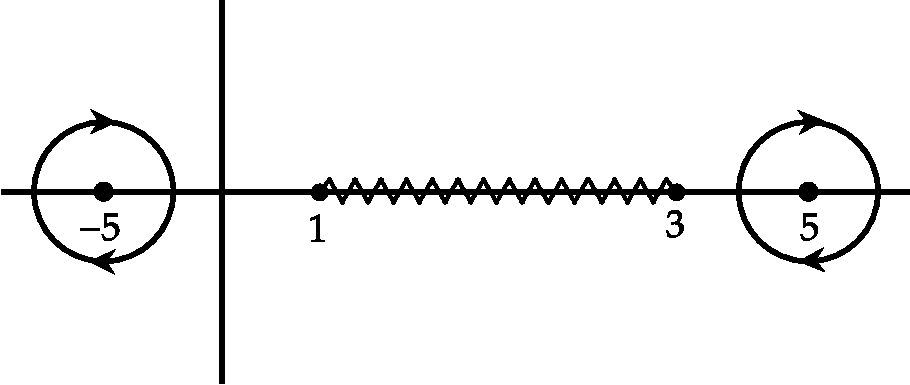
\includegraphics[height=3cm,width=6.5cm]{diagram-20211005(5)-crop}
		\end{figure}
		\task[\textbf{C.}] \begin{figure}[H]
			\centering
			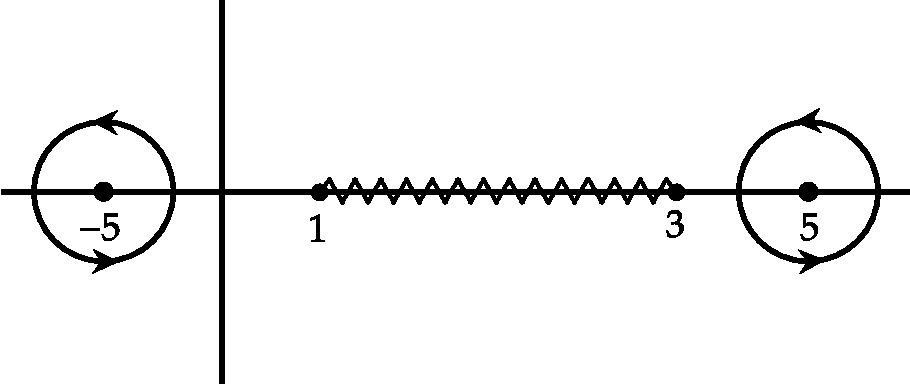
\includegraphics[height=3cm,width=6.5cm]{diagram-20211005(6)-crop}
		\end{figure}
		\task[\textbf{D.}] \begin{figure}[H]
			\centering
			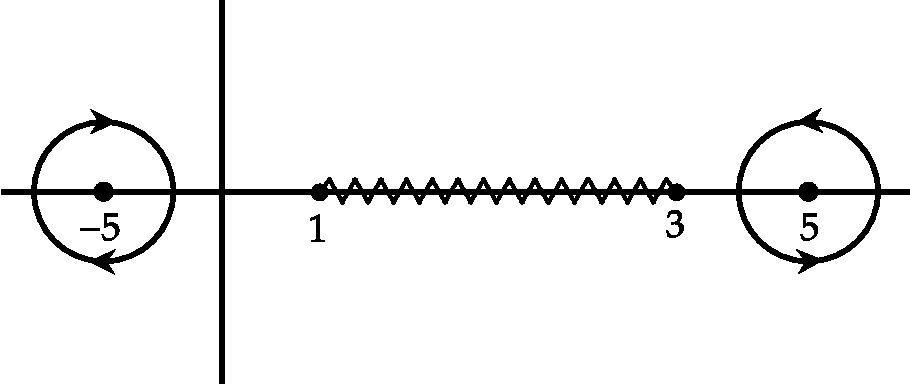
\includegraphics[height=3cm,width=6.5cm]{diagram-20211005(7)-crop}
		\end{figure}
	\end{tasks}
	\begin{answer}
		\begin{align*}
		\intertext{$z=1,3$ are branch points $\infty$ is not a branch point 1 branch cut 3}
		\end{align*}
		So the correct answer is \textbf{Option (C)}
	\end{answer}
	\item  Let $C$ be the circle of radius $\frac{\pi}{4}$ centered at $z=\frac{1}{4}$ in the complex $z$-plane that is traversed counter-clockwise. The value of the contour integral $\oint_{C} \frac{z^{2}}{\sin ^{2} 4 z} d z$ is
	{\exyear{NET/JRF(DEC-2019)}}
	\begin{tasks}(4)
		\task[\textbf{A.}] 0
		\task[\textbf{B.}] $\frac{i \pi^{2}}{4}$
		\task[\textbf{C.}] $\frac{i \pi^{2}}{16}$
		\task[\textbf{D.}] $\frac{i \pi}{4}$
	\end{tasks}
	\begin{answer}$\left. \right. $
		\begin{figure}[H]
			\centering
			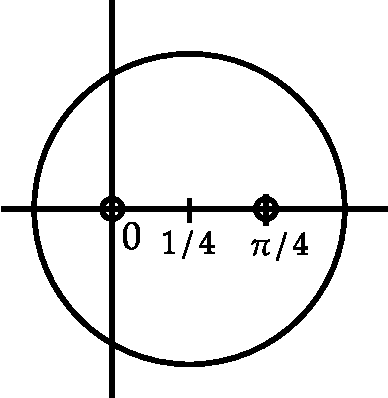
\includegraphics[height=3cm,width=3cm]{diagram-20211026(16)-crop}
		\end{figure}
		\begin{align*}
		f(z)&=\left(\frac{\pi}{\sin 4 z}\right)^{2}\\
		z_{0}&=0, \frac{\pi}{4}\text{ are poles}\\
		4 z&=n \pi, z=0, \frac{\pi}{4}
		\intertext{Others are outside the contour.}
		\text{Residue at }z&=0\text{ is }\left[\frac{\pi}{4 z-\frac{4^{3} z^{3}}{3 !}+\ldots}\right]^{2}\\
		&=\left[\frac{1}{4-\frac{4^{3} z^{2}}{3 !}+\ldots .}\right]^{2}\qquad \text{ No terms for } \frac{1}{z}, b_{1}=0\\
		&=\left[4-\frac{4^{3} z^{2}}{3 !}+\ldots .\right]^{-2}\\
		\text{Residue for }z&=\frac{\pi}{4}\\
		z-\frac{\pi}{4}&=t
		\intertext{$\sin (4 t+\pi)=-\sin 4 t \quad$ (But square so no effect)}
		&\left[\frac{t+\frac{\pi}{4}}{\sin 4\left(t+\frac{\pi}{4}\right)}\right]^{2}\\
		\left(\frac{t+\frac{\pi}{4}}{\sin 4 t}\right)^{2}&=\frac{t^{2}+\frac{\pi^{2}}{4}+2 t \cdot \frac{\pi}{4}}{\sin ^{2} 4 t}\\
		\frac{\pi}{2} \frac{t}{16 t^{2}[1-\ldots .]^{2}}&=\frac{\pi}{32 t}[1-\ldots .]^{-2} \text{(from first term)}\\
		b_{1}&=\frac{\pi}{32}\\
		\oint_{C} \frac{z^{2}}{\sin ^{2} 4 z} d z&=2 \pi i\left[0+\frac{\pi}{32}\right]=\frac{i \pi^{2}}{16}
		\end{align*}
		So the correct answer is \textbf{Option (C)}
	\end{answer}
	\item  A function of a complex variable $z$ is defined by the integral $f(z)=\oint_{\Gamma} \frac{w^{2}-2}{w-z} d w$, where $\Gamma$ is a circular contour of radius 3 , centred at origin, running counter-clockwise in the $w$ - plane. The value of the function at $z=(2-i)$ is
	{\exyear{NET/JRF(JUNE-2020)}}
	\begin{tasks}(4)
		\task[\textbf{A.}] 0
		\task[\textbf{B.}] $1-4 i$
		\task[\textbf{C.}]  $8 \pi+2 \pi \mathrm{i}$
		\task[\textbf{D.}] $-\frac{2}{\pi}-\frac{i}{2 \pi}$
	\end{tasks}
	\begin{answer}$\left. \right. $
		\begin{figure}[H]
			\centering
			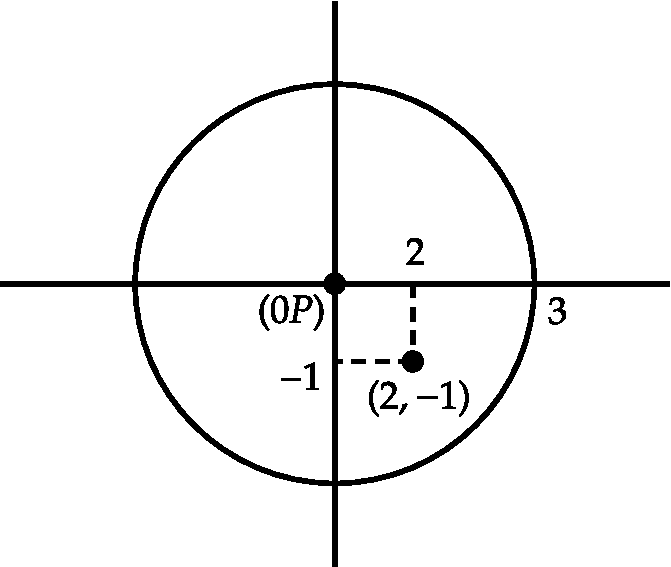
\includegraphics[height=4cm,width=4.6cm]{diagram-20211027-crop}
		\end{figure}
		\begin{align*}
		f(z)&=\oint_{\Gamma} \frac{w^{2}-2}{w-z} d w\\
		\omega&=z\text{ is a simple pole.}\\
		\text{Residue }\lim _{\omega \rightarrow z}(\omega-z) \frac{\left(\omega^{2}-2\right)}{(\omega-z)}&=(2-i)^{2}-2 \\&=4-1-4 i-2=(1-4 i)\\
		f(z)&=\oint_{\Gamma} \frac{w^{2}-2}{w-z} d w=2 \pi i(1-4 i)=2 \pi i+8 \pi
		\end{align*}
		So the correct answer is \textbf{Option (C)}
	\end{answer}
\end{enumerate}
\colorlet{ocre1}{ocre!70!}
\colorlet{ocrel}{ocre!30!}
\setlength\arrayrulewidth{1pt}
\begin{table}[H]
	\centering
	\arrayrulecolor{ocre}
	\begin{tabular}{|p{1.5cm}|p{1.5cm}||p{1.5cm}|p{1.5cm}|}
		\hline
		\multicolumn{4}{|c|}{\textbf{Answer key}}\\\hline\hline
		\rowcolor{ocrel}Q.No.&Answer&Q.No.&Answer\\\hline
		1&\textbf{C} &2&\textbf{B}\\\hline 
		3&\textbf{B} &4&\textbf{A} \\\hline
		5&\textbf{A} &6&\textbf{D} \\\hline
		7&\textbf{A}&8&\textbf{-}\\\hline
		9&\textbf{C}&10&\textbf{A}\\\hline
		11&\textbf{C} &12&\textbf{-}\\\hline
		13&\textbf{A}&14&\textbf{B}\\\hline
		15&\textbf{C}&16&\textbf{B}\\\hline
		17&\textbf{C} &18&\textbf{A}\\\hline
		19&\textbf{B}&20&\textbf{B}\\\hline
		21&\textbf{C}&22&\textbf{C}\\\hline
		23&\textbf{C}& &\\\hline
		
	\end{tabular}
\end{table}
\newpage
\begin{abox}
	Practise Set-2
\end{abox}
\begin{enumerate}[label=\color{ocre}\textbf{\arabic*.}]
	\item  The value of the integral $\oint_{C} \frac{e^{z} \sin (z)}{z^{2}} d z$, where the contour $C$ is the unit circle: $|z-2|=1$, is
	{\exyear{GATE 2010}}
	\begin{tasks}(4)
		\task[\textbf{A.}] $2 \pi i$
		\task[\textbf{B.}] $4 \pi i$
		\task[\textbf{C.}] $\pi i$
		\task[\textbf{D.}] 0
	\end{tasks}
	\begin{answer}
		\begin{align*}
		\intertext{$|z-2|=1 \Rightarrow 1<z<3$ i.e. the pole $z=0$ does not lie inside the contour.}
		\therefore \quad \oint_{C} \frac{e^{z} \sin z}{z^{2}} d z=2 \pi i \times 0=0 .
		\end{align*}
		So the correct answer is \textbf{Option (D)}
	\end{answer}
	\item Which of the following statements is TRUE for the function $f(z)=\frac{z \sin z}{(z-\pi)^{2}}$ ?
	{\exyear{GATE 2011}}
	\begin{tasks}(1)
		\task[\textbf{A.}] $f(z)$ is analytic everywhere in the complex plane
		\task[\textbf{B.}] $f(z)$ has a zero at $z=\pi$
		\task[\textbf{C.}] $f(z)$ has a pole of order 2 at $z=\pi$
		\task[\textbf{D.}] $f(z)$ has a simple pole at $z=\pi$
	\end{tasks}
	\begin{answer}
		\begin{align*}
		f(z)=\frac{z \sin z}{(z-\pi)^{2}}\text{ has a pole of order 2 at }z=\pi
		\end{align*}
		So the correct answer is \textbf{Option (C)}
	\end{answer}
	\item For the function $f(z)=\frac{16 z}{(z+3)(z-1)^{2}}$, the residue at the pole $z=1$ is (your answer should be an integer)-------
	{\exyear{GATE 2013}}
	\begin{answer}
		\begin{align*}
		\text{	At }z&=1,\text{ pole is of order 2 .} \\&\text{So, residue is }\frac{1}{\lfloor-1} \frac{d^{2-1}}{d z^{2-1}}\left[\frac{(z-1)^{2} 16 z}{(z+3)(z-1)^{2}}\right]_{z=1}=3
		\end{align*}
	\end{answer}
	\item The value of the integral
	$$
	\oint_{C} \frac{z^{2}}{e^{z}+1} d z
	$$
	where $C$ is the circle $|z|=4$, is
	{\exyear{GATE 2014}}
	\begin{tasks}(4)
		\task[\textbf{A.}] $2 \pi i$
		\task[\textbf{B.}] $2 \pi^{2} i$
		\task[\textbf{C.}]  $4 \pi^{3} i$
		\task[\textbf{D.}] $4 \pi^{2} i$
	\end{tasks}
	\begin{answer}
		\begin{align*}
		\text{	Pole }e^{z}&=-1 \Rightarrow e^{z}=e^{i(2 m+1) \pi}\text{ where }m=0,1,2,3 \ldots \ldots\\
		\text{For }z&=i \pi,\text{ Res }=\lim _{z=i \pi} \frac{\phi(z)}{\phi^{\prime}(z)}\\&=-\frac{\pi^{2}}{e^{i \pi}}=\pi^{2}\\
		\text{Similarly, for }z&=-i \pi,\text{ Res }=\pi^{2}\\
		\therefore I&=2 \pi i\left(\pi^{2}+\pi^{2}\right)=4 \pi^{3} i
		\end{align*}
			So the correct answer is \textbf{Option (C)}
	\end{answer}
	\item Consider a complex function $f(z)=\frac{1}{z\left(z+\frac{1}{2}\right) \cos (z \pi)}$. Which one of the following statements is correct?
	{\exyear{GATE 2015}}
	\begin{tasks}(1)
		\task[\textbf{A.}] $f(z)$ has simple poles at $z=0$ and $z=-\frac{1}{2}$
		\task[\textbf{B.}] $f(z)$ has second order pole at $z=-\frac{1}{2}$
		\task[\textbf{C.}] $f(z)$ has infinite number of second order poles
		\task[\textbf{D.}] $f(z)$ has all simple poles
	\end{tasks}
	\begin{answer}
		\begin{align*}
		f(z)&=\frac{1}{z\left(z+\frac{1}{2}\right) \cos (z \pi)}\\
		\text{	For $n^{t h}$ order pole, Res. }&=\lim _{z \rightarrow a}(z-a)^{n} f(z)=\text{ finite}\\
		\text{At }z&=0, \lim _{z \rightarrow 0} z f(z)=\text{ finite }\\\Rightarrow z&=0\text{ is a simple pole.}\\
		\text{At }z&=-\frac{1}{2}, \lim _{z \rightarrow-\frac{1}{2}} \frac{\left(z+\frac{1}{2}\right)^{2}}{z\left(z+\frac{1}{2}\right) \cos z \pi}=\lim _{z \rightarrow-\frac{1}{2}} \frac{\left(z+\frac{1}{2}\right)}{z \cos z \pi}\\&=\lim _{z \rightarrow-\frac{1}{2}} \frac{1}{1 . \cos z \pi+z . \pi(-\sin z \pi)}\\
		&=\lim _{z \rightarrow-\frac{1}{2}} \frac{1}{\cos z \pi-z \pi \sin z \pi}=\frac{1}{-\frac{\pi}{2}}\\&=-\frac{2}{\pi}=\text{ finite}\\
		\Rightarrow f(z)\text{ has second order pole at }z&=-\frac{1}{2}
		\end{align*}
		So the correct answer is \textbf{Option (A)}
	\end{answer}
	\item  Consider $w=f(z)=u(x, y)+i v(x, y)$ to be an analytic function in a domain $D$. Which one of the following options is NOT correct?
	{\exyear{GATE 2015}}
	\begin{tasks}(1)
		\task[\textbf{A.}] $u(x, y)$ satisfies Laplace equation in D
		\task[\textbf{B.}]  $v(x, y)$ satisfies Laplace equation in $D$
		\task[\textbf{C.}] $\int_{1}^{z_{2}} f(z) d z$ is dependent on the choice of the contour between $z_{1}$ and $z_{2}$ in $D$
		\task[\textbf{D.}]  $f(z)$ can be Taylor expended in $D$
	\end{tasks}
	\begin{answer}
		\begin{align*}
		w&=f(z)=u(x, y)+i v(x, y)\text{ to be an analytic function in a domain }D, \int_{z_{1}}^{z_{2}} f(z) d z\text{ is}\\
		&\text{independent of the choice of the contour between }z_{1}\text{ and }z_{2}\text{ in }D.
		\end{align*}
		So the correct answer is \textbf{Option (C)}
	\end{answer}
	\item A function $y(z)$ satisfies the ordinary differential equation $y^{\prime \prime}+\frac{1}{z} y^{\prime}-\frac{m^{2}}{z^{2}} y=0$, where\\
	$m=0,1,2,3, \ldots . .$ Consider the four statements P, Q, R, S as given below.\\
	$\mathrm{P}: z^{m}$ and $z^{-m}$ are linearly independent solutions for all values of $m$\\
	Q: $z^{m}$ and $z^{-m}$ are linearly independent solutions for all values of $m>0$\\
	$\mathrm{R}$ : $\ln z$ and 1 are linearly independent solutions for $m=0$\\
	S: $z^{m}$ and $\ln z$ are linearly independent solutions for all values of $m$\\
	The correct option for the combination of valid statements is
	{\exyear{GATE 2015}}
	\begin{tasks}(4)
		\task[\textbf{A.}] P, R and S only
		\task[\textbf{B.}]  P and R only
		\task[\textbf{C.}] $\mathrm{Q}$ and $\mathrm{R}$ only
		\task[\textbf{D.}] $\mathrm{R}$ and $\mathrm{S}$ only
	\end{tasks}
	\begin{answer}
		\begin{align*}
		y^{\prime \prime}+\frac{1}{z} y^{\prime}-\frac{m^{2}}{z^{2}} y&=0 \Rightarrow z^{2} y^{\prime \prime}+z y^{\prime}-m^{2} y\\&=0, m=0,1,2,3, \ldots, \quad z=e^{x}, D=\frac{d}{d x}\\
		\text{	If }m&=0 ; \quad z^{2} y^{\prime \prime}+z y^{\prime}=0,[D(D-1)+D] y\\&=0 \Rightarrow\left[D^{2}-D+D\right] y=0\\
		D^{2} y&=0 \Rightarrow y=c_{1}+c_{2} x \Rightarrow y\\&=c_{1}+c_{2} \ln z \quad \text{( $R$ is correct)}\\
		\text{And if }m &\neq 0, m>0,\text{ then }m \neq 0,\text{ then }\left(D^{2}-m^{2}\right) y\\&=0 \Rightarrow D=\pm m\\
		y&=c_{1} e^{m x}+c_{2} e^{-m x}=c_{1} e^{m \log z}+c_{2} e^{-m \log z}\\&=c_{1} z^{m}+c_{2} z^{-m}\\
		\text{or if }m &\neq 0, m>0,\text{ then}\\
		y&=c_{1} \cosh (m \log (z))+i c_{2} \sinh (m \log (x)), \quad m>0
		\end{align*}
		So the correct answer is \textbf{Option (C)} 
	\end{answer}
	\item  Which of the following is an analytic function of $z$ everywhere in the complex plane?
	{\exyear{GATE 2016}}
	\begin{tasks}(4)
		\task[\textbf{A.}] $z^{2}$
		\task[\textbf{B.}]  $\left(z^{*}\right)^{2}$
		\task[\textbf{C.}] $|z|^{2}$
		\task[\textbf{D.}] $\sqrt{z}$
	\end{tasks}
	\begin{answer}
		\begin{align*}
		z^{2}&=(x+i y)^{2}=x^{2}-y^{2}+i(2 x y) \Rightarrow u\\&=x^{2}-y^{2}\text{ and }v=2 x y\\
		\text{Cauchy Riemann equations }\frac{\partial u}{\partial x}&=\frac{\partial v}{\partial y}=2 x, \quad \frac{\partial v}{\partial x}=-\frac{\partial u}{\partial y}=2 y\text{ satisfies.}
		\end{align*}
		So the correct answer is \textbf{Option (A)}
	\end{answer}
	\item The contour integral $\oint \frac{d z}{1+z^{2}}$ evaluated along a contour going from $-\infty$ to $+\infty$ along the
	real axis and closed in the lower half-plane circle is equal to............... (up to two decimal places).
	{\exyear{GATE 2017}}
	\begin{answer}
		\begin{align*}
		\oint_{c} \frac{1}{1+z^{2}} d z&=\int_{-\infty}^{+\infty} \frac{1}{1+x^{2}} d x+\oint_{c} \frac{1}{1+z^{2}} d z\\
		\text{Poles, }1+z^{2}&=0 \Rightarrow z=\pm i, \quad z=-i\text{ is inside }C\\
		\therefore \operatorname{Res}(z=-i)&=\lim _{z \rightarrow-i}(z+i) \frac{1}{(z-i)(z+i)}\\&=\frac{1}{-i-i}=\frac{1}{-2 i}\\
		\int_{-\infty}^{+\infty} \frac{1}{1+x^{2}} d x&=-\frac{1}{2 i} \times-2 \pi i=\pi
		\intertext{(Since, here we use lower half plane i.e., we traversed in clockwise direction, hence we have to take $-2 \pi i$ )}
		\end{align*}
	\end{answer}
	\item The imaginary part of an analytic complex function is $v(x, y)=2 x y+3 y .$ The real part of the function is zero at the origin. The value of the real part of the function at $1+i$ is ................. (up to two decimal places)
	{\exyear{GATE 2017}}
	\begin{answer}
		\begin{align*}
		\intertext{Solution: The imaginary part of the given analytic function is $v(x, y)=2 x y+3 y .$ From the
			Cauchy - Riemann condition}
		\frac{\partial v}{\partial y}&=\frac{\partial u}{\partial x}=2 x+3
		\intertext{Integrating partially gives}
		u(x, y)&=x^{2}+3 x+g(y)\\
		\intertext{From the second Cauchy - Riemann condition}
		\frac{\partial u}{\partial y}&=-\frac{\partial v}{\partial x},\text{ we obtain} \frac{\partial u}{\partial y}\\&=-2 y, \mu(x, y)=-y^{2}+g(x)\\
		\frac{d g(y)}{d y}&=-2 y \Rightarrow g(y)=-y^{2}+c\\
		\text{	Hence, }u(x, y)&=x^{2}+3 x-y^{2}+c
		\intertext{Since, the real part of the analytic function is zero at the origin.}
		\text{Hence, }0&=0+0-0+c \Rightarrow c=0\\
		\text{Thus, }u(x, y)&=x^{2}+3 x-y^{2}\\
		\therefore f(z)&=\left(x^{2}+3 x-y^{2}\right)+i(2 x y+3 y)
		\intertext{Thus, the value of real part when}
		z&=1+i, i.e. x=1\text{ and }y=1\text{ is }u(x, y)\\&=(1)^{2}+3(1)-1=3
		\end{align*}
	\end{answer}
	\item The absolute value of the integral
	$$
	\int \frac{5 z^{3}+3 z^{2}}{z^{2}-4} d z
	$$
	over the circle $|z-1.5|=1$ in complex plane, is $\ldots$ (up to two decimal places).
	{\exyear{GATE 2018}}
	\begin{answer}
		\begin{align*}
		f(z)&=\frac{5 z^{3}+3 z^{2}}{(z-2)(z+2)}\\
		\text{Pole, }z&=2,-2\\
		z&=-2 \text{ is outside the center}\\
		|-2-1.5|>1&\text{So, will not be considered}\\
		\text{	Now, }\operatorname{Re} s(2)&=\lim _{z \rightarrow 2}(z-2) \frac{\left(5 z^{3}+3 z^{2}\right)}{(z-2)(z+2)}\\&=\frac{52^{3}+32^{2}}{4}=\frac{40+12}{4}=13\\
		I&=2 \pi i \times residue =2 \pi i \times 13\\&=26 \times 3.14 \Rightarrow I=81.64
		\end{align*}
	\end{answer}
	\item The pole of the function $f(z)=\cot z$ at $z=0$ is
	{\exyear{GATE 2019}}
	\begin{tasks}(2)
		\task[\textbf{A.}] A removable pole
		\task[\textbf{B.}] An essential singularity
		\task[\textbf{C.}]  A simple pole
		\task[\textbf{D.}] A second order pole
	\end{tasks}
	\begin{answer}
		\begin{align*}
		f(z)&=\cot z\text{ at }z=0\\
		f(z)&=\frac{1}{\tan z} \quad z=0\text{ is a simple pole }\\f(z)&=\frac{1}{z}\left[1-\frac{1}{3} z^{2}+\ldots .\right]
		\end{align*}
		So the correct answer is \textbf{Option (C)}
	\end{answer}
	\item The value of the integral $\int_{-\infty}^{\infty} \frac{\cos (k x)}{x^{2}+a^{2}} d x$, where $k>0$ and $a>0$, is
	{\exyear{GATE 2019}}
	\begin{tasks}(4)
		\task[\textbf{A.}] $\frac{\pi}{a} e^{-k a}$
		\task[\textbf{B.}] $\frac{2 \pi}{a} e^{-k a}$
		\task[\textbf{C.}] $\frac{\pi}{2 a} e^{-k a}$
		\task[\textbf{D.}] $\frac{3 \pi}{2 a} e^{-k a}$
	\end{tasks}
	\begin{answer}
		\begin{align*}
		&\int_{-\infty}^{\infty} \frac{\cos k x}{x^{2}+a^{2}} d x\\
		f(z)&=\frac{e^{i k x}}{z^{2}+a^{2}}=\frac{e^{i k z}}{(z+i a)(z-i a)}\\
		I&=\operatorname{Re} .2 \pi i \times \frac{e^{i k(i a)}}{2 i a}=\frac{\pi e^{-k a}}{a}
		\end{align*}
		So the correct answer is \textbf{Option (A)}
	\end{answer}
\item The value of the integral $\int_{0}^{\infty} \frac{\ln x}{\left(x^{2}+1\right)^{2}} d x$ is
{\exyear{ JEST 2012}}
 \begin{tasks}(2)
	\task[\textbf{a.}]0
	\task[\textbf{b.}]$\frac{-\pi}{4}$
	\task[\textbf{c.}] $\frac{-\pi}{2}$
	\task[\textbf{d.}] $\frac{\pi}{2}$
\end{tasks}
\begin{answer}$\left. \right. $
	\begin{figure}[H]
		\centering
		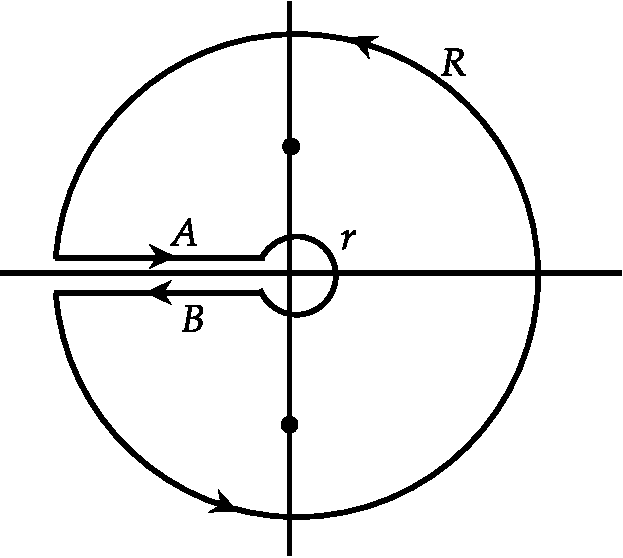
\includegraphics[height=4cm,width=4.6cm]{JEST 01 2012}
	\end{figure}
	\begin{align*}
	\int_{0}^{\infty} \frac{\ln x}{\left(x^{2}+1\right)^{2}} d x&=\int_{0}^{\infty} \frac{\ln z}{\left(z^{2}+1\right)^{2}} d z\\
	\text{Let us consider new function }f(z)&=\left(\frac{\ln z}{z^{2}+1}\right)^{2},\text{ then }I=\int_{0}^{\infty}\left(\frac{\ln z}{z^{2}+1}\right)^{2} d z\\
\text{	Pole at }z&=\pm i\text{ is simple pole of second order.}\\
\text{	Residue at }z&=i\text{ is}\\
&=\frac{d}{d z}(z-i)^{2} \frac{(\ln z)^{2}}{(z-i)^{2}(z+i)^{2}}=\frac{d}{d z} \frac{(\ln z)^{2}}{(z+i)^{2}}\\
&=\frac{(z+i)^{2} 2(\ln z) \cdot \frac{1}{z}-(\ln z)^{2} \cdot 2(z+i)}{(z+i)^{4}}=\frac{(z+i) 2 \ln (z) \frac{1}{z}-(\ln z)^{2} \cdot 2}{(z+i)^{3}}\\
&=\frac{(2 i) 2 \times \frac{1}{i} \ln i-(\ln i)^{2} \cdot 2}{(2 i)^{3}}=\frac{4 \frac{i \pi}{2}-\left(\frac{i \pi}{2}\right)^{2} \times 2}{-8 i}=\frac{2 \pi i+\frac{\pi^{2}}{2}}{-8 i}\\
\left.\Rightarrow \operatorname{Res}\right|_{z=i}&=\frac{-\pi}{4}+\frac{\pi^{2}}{16} i\\
\text{Similarly, at }z&=-i ;\left.\operatorname{Res}\right|_{z=-i}=\frac{-\pi}{4}-\frac{\pi^{2}}{16} i\\
I&=\int_{0}^{\infty}\left(\frac{\ln z}{z^{2}+1}\right)^{2} d z=2 \pi i\left(\frac{-\pi}{4}+\frac{\pi^{2}}{16} i-\frac{\pi}{4}-\frac{\pi^{2}}{16} i\right)=-\pi^{2} i\\
-\pi^{2} i&=\left(\int_{R} \int_{A} \int_{B}\right) f(z) d z=\left(\iint_{A B}\right) f(z) d z ;\qquad \left[\because \int_{A B}\right.\text{ vanish }]\\
\text{Along path }A ;& \quad z=-x+i \varepsilon\text{ and along path }B ; \quad z=-x-i \varepsilon\\
\text{Thus }-\pi^{2} i&=\left(\iint_{A B}\right) f(z) d z=-\int_{-\infty}^{0}\left[\frac{\ln (-x+i \varepsilon)}{(-x+i \varepsilon)^{2}+1}\right] d x-\int_{0}^{\infty}\left[\frac{\ln (-x-i \varepsilon)}{(-x-i \varepsilon)^{2}+1}\right] d x\\
\Rightarrow-\pi^{2} i&=\int_{0}^{\infty}\left[\frac{\ln (-x+i \varepsilon)}{(-x+i \varepsilon)^{2}+1}\right]^{2} d x-\int_{0}^{\infty}\left[\frac{\ln (-x-i \varepsilon)}{(-x-i \varepsilon)^{2}+1}\right]^{2} d x\\
\Rightarrow-\pi^{2} i&=\int_{0}^{\infty}\left[\frac{\ln (x)+i \pi}{1+x^{2}}\right]^{2} d x-\int_{0}^{\infty}\left[\frac{\ln (x)-i \pi}{1+x^{2}}\right]^{2} d x ; \quad \varepsilon \rightarrow 0\\
\Rightarrow-\pi^{2} i&=\int_{0}^{\infty} \frac{(\ln (x)+i \pi)^{2}-(\ln (x)-i \pi)^{2}}{\left(1+x^{2}\right)^{2}} d x\\&=4 \pi i \int_{0}^{\infty} \frac{\ln x}{\left(x^{2}+1\right)^{2}} \Rightarrow \int_{0}^{\infty} \frac{\ln x}{\left(x^{2}+1\right)^{2}}=\frac{-i \pi^{2}}{4 \pi i}=\frac{-\pi}{4}
	\end{align*}
		So the correct answer is \textbf{Option (B)}
\end{answer}
\item Compute $\lim _{z \rightarrow 0} \frac{\operatorname{Re}\left(z^{2}\right)+\operatorname{Im}\left(z^{2}\right)}{z^{2}}$
{\exyear{ JEST 2013}}
 \begin{tasks}(2)
	\task[\textbf{a.}] The limit does not exist
	\task[\textbf{b.}]1
	\task[\textbf{c.}]$-i$
	\task[\textbf{d.}] $-1$
\end{tasks}
\begin{answer}
	\begin{align*}
	\lim _{z \rightarrow 0} \frac{\operatorname{Re}\left(z^{2}\right)+\operatorname{Im}\left(z^{2}\right)}{z^{2}}&=\lim _{z \rightarrow 0} \frac{x^{2}-y^{2}+2 x y}{x^{2}-y^{2}+2 i x y}=\lim _{y=0 \atop x \rightarrow 0} \frac{x^{2}-y^{2}+2 x y}{x^{2}-y^{2}+2 i x y}=1\\
	\lim _{x=0 \atop y \rightarrow 0} \frac{x^{2}-y^{2}+2 x y}{x^{2}-y^{2}+2 i x y}&=1\text{ and }\lim _{y=x \atop x \rightarrow 0} \frac{x^{2}-y^{2}+2 x y}{x^{2}-y^{2}+2 i x y}=-i
	\end{align*}
		So the correct answer is \textbf{Option (A)}
\end{answer}
\item The value of limit
$$
\lim _{z \rightarrow i} \frac{z^{10}+1}{z^{6}+1}
$$
is equal to
{\exyear{ JEST 2014}}
 \begin{tasks}(2)
	\task[\textbf{a.}]1
	\task[\textbf{b.}]0
	\task[\textbf{c.}] $\frac{-10}{3}$
	\task[\textbf{d.}] $\frac{5}{3}$
\end{tasks}
\begin{answer}
	\begin{align*}
	\lim _{z \rightarrow i} \frac{z^{10}+1}{z^{6}+1}=\lim _{z \rightarrow i} \frac{10 z^{9}}{6 z^{5}}=\lim _{z \rightarrow i} \frac{10 z^{4}}{6}=\frac{10}{6}=\frac{5}{3}
	\end{align*}
		So the correct answer is \textbf{Option (D)}
\end{answer}
\item The value of integral
$$
I=\oint \frac{\sin z}{2 z-\pi} d z
$$
with $c$ a circle $|z|=2$, is
{\exyear{ JEST 2014}}
 \begin{tasks}(2)
	\task[\textbf{a.}] 0
	\task[\textbf{b.}]$2 \pi i$
	\task[\textbf{c.}] $\pi i$
	\task[\textbf{d.}]  $-\pi i$
\end{tasks}
\begin{answer}
	\begin{align*}
	I&=\oint_{C} \frac{\sin z}{2 z-\pi},\text{ for pole }2 z-\pi=0 \Rightarrow z=\frac{\pi}{2}\\
\text{	Residue at }z&=\frac{\pi}{2}
	\because|z|=2\text{, so pole will lie within the contour}\\
	I&=\oint_{C} \frac{e^{i z}}{2\left(z-\frac{\pi}{2}\right)}=\sum R \times 2 \pi i\\
	\left.\operatorname{Res}\right|_{z=\frac{\pi}{2}}&=\frac{\left(z-\frac{\pi}{2}\right) e^{i z}}{2\left(z-\frac{\pi}{2}\right)}=\frac{e^{i \pi / 2}}{2}=\frac{i}{2}\text{ (taking imaginary part); Residue }=\frac{1}{2}\\
	\text{Now, }I&=\frac{1}{2} \times 2 \pi i=\pi i
	\end{align*}
		So the correct answer is \textbf{Option (C)}
\end{answer}
\item Given an analytic function $f(z)=\phi(x, y)+i \psi(x, y)$, where $\phi(x, y)=x^{2}+4 x-y^{2}+2 y$
If $C$ is a constant, which of the following relations is true?
{\exyear{ JEST 2015}}
 \begin{tasks}(2)
	\task[\textbf{a.}]$\psi(x, y)=x^{2} y+4 y+C$
	\task[\textbf{b.}]$\psi(x, y)=2 x y-2 x+C$
	\task[\textbf{c.}]$\psi(x, y)=2 x y+4 y-2 x+C$
	\task[\textbf{d.}] $\psi(x, y)=x^{2} y-2 x+C$
\end{tasks}
\begin{answer}
	\begin{align}
	u&=\phi(x, y)=x^{2}+4 x-y^{2}+2 y, v=\psi\notag\\
	\text{From C.R. equation, }\frac{\partial u}{\partial x}&=\frac{\partial v}{\partial y}, \Rightarrow \frac{\partial \phi}{\partial x}=\frac{\partial \psi}{\partial y}, \frac{\partial u}{\partial y}=-\frac{\partial v}{\partial x} \Rightarrow \frac{\partial \phi}{\partial y}=-\frac{\partial \psi}{\partial x}\notag\\
	\text{Now, }\frac{\partial \phi}{\partial x}&=2 x+4=\frac{\partial \psi}{\partial y}\notag\\
	\Rightarrow \psi&=2 x y+4 y+f(x)\label{CN 01}\\
	\text{and }\frac{\partial \phi}{\partial y}&=-2 y+2 \Rightarrow \frac{\partial \psi}{\partial x}=+2 y-2\notag\\
	\psi&=2 x y+2 x+f(y)\label{CN 02}\\
	\text{From (\ref{CN 01}) and (\ref{CN 02}), }&2 x y+4 y+f(x)=2 x y-2 x+f(y)\notag\\
	f(x)&=-2 x, \quad f(y)=4 y \notag\\
	\psi&=2 x y+4 y-2 x+c\notag
	\end{align}
		So the correct answer is \textbf{Option (C)}
\end{answer}
\item Which one is the image of the complex domain $\{z \mid x y \geq 1, x+y>0\}$ under the mapping $f(z)=z^{2}$, if $z=x+i y ?$
{\exyear{ JEST 2017}}
 \begin{tasks}(2)
	\task[\textbf{a.}] $\{z \mid x y \geq 1, x+y>0\}$
	\task[\textbf{b.}]$\{z \mid x \geq 2, x+y>0\}$
	\task[\textbf{c.}]$\{z \mid y \geq 2 \forall x\}$
	\task[\textbf{d.}] $\{z \mid y \geq 1 \forall x\}$
\end{tasks}
\item The integral $I=\int_{1}^{\infty} \frac{\sqrt{x-1}}{(1+x)^{2}} d x$ is
{\exyear{ JEST 2017}}
 \begin{tasks}(2)
	\task[\textbf{a.}]$\frac{\pi}{\sqrt{2}}$
	\task[\textbf{b.}]$\frac{\pi}{2 \sqrt{2}}$
	\task[\textbf{c.}]$\frac{\sqrt{\pi}}{2}$
	\task[\textbf{d.}]$\sqrt{\frac{\pi}{2}}$
\end{tasks}
\begin{answer}
	\begin{align*}
	I&=\int_{1}^{\infty} \frac{\sqrt{x-1}}{(1+x)^{2}} d x\\
\text{	Put,} x&=\left(1+z^{2}\right), d x=2 z d z\\
	\text{Hence, }I&=\int_{0}^{\infty} \frac{2 z^{2} d z}{\left(2+z^{2}\right)^{2}}\\
	\text{Here poles, }\left(2+z^{2}\right)&=0 \Rightarrow(z+i \sqrt{2})(z-i \sqrt{2})=0\\
\text{	Only }&(z=i \sqrt{2})\text{ poles is allowed}\\
\text{Then }R(i \sqrt{2})&=\lim _{z \rightarrow i \sqrt{2}} \frac{1}{\sqrt{2-1}} \frac{d}{d z}\left[\frac{2 z^{2}(z-i \sqrt{2})^{2}}{(z-i \sqrt{2})^{2}(z+i \sqrt{2})^{2}}\right]\\
&=\lim _{z \rightarrow i \sqrt{2}}\left[\frac{(z+i \sqrt{2})^{2} \cdot 4 z-2 z^{2} \cdot 2(z+i \sqrt{2})}{(z+i \sqrt{2})^{4}}\right]\\
&=\frac{(2 i \sqrt{2})^{2} \times 4(i \sqrt{2})-2(i \sqrt{2})^{2} \cdot 2(2 i \sqrt{2})}{(2 i \sqrt{2})^{4}}\\&=-\frac{32 \sqrt{2} i+16 \sqrt{2} i}{64}=-\frac{16 \sqrt{2} i}{64}=-\frac{i}{2 \sqrt{2}}\\
\text{Hence, }\int_{-\infty}^{\infty} \frac{2 z^{2}}{\left(2+z^{2}\right)^{2}} d z&=2 \pi i\left(-\frac{i}{2 \sqrt{2}}\right)=\frac{\pi}{\sqrt{2}}\\
\Rightarrow \int_{0}^{\infty} \frac{2 z^{2}}{\left(2+z^{2}\right)^{2}} d z&=\frac{\pi}{2 \sqrt{2}} \Rightarrow \int_{i}^{\infty} \frac{\sqrt{x-1}}{(1+x)^{2}} d x=\frac{\pi}{2 \sqrt{2}}
	\end{align*}
	So the correct answer is \textbf{Option (B)}
\end{answer}
\item The integral
$$
\int_{-\infty}^{\infty} \frac{\cos x}{x^{2}+1} d x \text { is }
$$
{\exyear{ JEST 2018}}
 \begin{tasks}(2)
	\task[\textbf{a.}]$\frac{\pi}{e}$
	\task[\textbf{b.}] $\pi e^{-2}$
	\task[\textbf{c.}]$\pi$
	\task[\textbf{d.}] zero
\end{tasks}
\begin{answer}
	\begin{align*}
	f(z)&=\frac{e^{i z}}{z^{2}+1}=\frac{e^{i z}}{(z+i)(z-i)}\\
	\int_{-\infty}^{\infty} \frac{\cos x}{x^{2}+1} d x&=\operatorname{Re} 2 \pi i \times \frac{e^{i \cdot i}}{z i}=\frac{\pi}{e}
	\end{align*}
		So the correct answer is \textbf{Option (A)}
\end{answer}
\item Consider the function $f(x, y)=|x|-i|y| .$ In which domain of the complex plane is this function analytic?
{\exyear{ JEST 2019}}
 \begin{tasks}(2)
	\task[\textbf{a.}]First and second quadrants
	\task[\textbf{b.}]Second and third quadrants
	\task[\textbf{c.}]Second and fourth quadrants
	\task[\textbf{d.}]  Nowhere
\end{tasks}
\begin{answer}
	\begin{align*}
	 f(x, y)&=|x|-i|y|\\
	f(x, y)&=x-i y=\bar{z}\\
	f(x, y)&=-x-i y=-z\\
	f(x, y)&=-x+i y=-\bar{z}\\
	f(x, y)&=x+i y=z
	\intertext{We know $\bar{z}$ is not analytic and $z$ and $-z$ are analytic. }
	\end{align*}
	So the correct answer is \textbf{Option (C)}
\end{answer}
\end{enumerate}
 \colorlet{ocre1}{ocre!70!}
\colorlet{ocrel}{ocre!30!}
\setlength\arrayrulewidth{1pt}
\begin{table}[H]
	\centering
	\arrayrulecolor{ocre}
	\begin{tabular}{|p{1.5cm}|p{1.7cm}||p{1.5cm}|p{1.5cm}|}
		\hline
		\multicolumn{4}{|c|}{\textbf{Answer key}}\\\hline\hline
		\rowcolor{ocrel}Q.No.&Answer&Q.No.&Answer\\\hline
		1&\textbf{D} &2&\textbf{C}\\\hline 
		3&\textbf{3(NAT)} &4&\textbf{C} \\\hline
		5&\textbf{A} &6&\textbf{C} \\\hline
		7&\textbf{C}&8&\textbf{A}\\\hline
		9&\textbf{$\pi$(NAT)}&10&\textbf{3(NAT)}\\\hline
		11&\textbf{81.64(NAT)} &12&\textbf{C}\\\hline
		13&\textbf{A}& 14&\textbf{B}\\\hline
		15&\textbf{A}&16 &\textbf{D}\\\hline
		17&\textbf{C}&18&\textbf{C}\\\hline
		19&\textbf{-} &20&\textbf{B}\\\hline
		21&\textbf{A}&22&\textbf{C}\\\hline
	\end{tabular}
\end{table}
\chapter{Complex Numbers}
A simple algebraic equation like $x^{2}=-1$ may not have a real solution. Introducing complex numbers validates the existence of 'root' for every polynomial with a positive degree . Which then proves the fundamental theorem of algebra. The idea of complex numbers are widely used in Physics and Mathematics.
\begin{definition}
	A number of the form {${x+i y}$} , where $x$ and $y$ are real numbers and $i=\sqrt{(-1)},$ is called a complex number.
\end{definition}
	\textbf{\large Real Part\ \hspace{1.08cm}:} $x$ is called the real part of the complex number,  $x+i y$ and is written as,\ ${{R(x+i y)}}$.\\\\ 
	\textbf{\large Imaginary Part\ :} $y$ is called the imaginary part of the complex number and is written as,\ ${I(x+i y)}$.
	\section{Representation of a Complex number}
The point whose cartesian coordinates are $(x, y)$ uniquely
represents the complex number, {${z=x+i y}$} on the complex plane $z$. The diagram in which this representation is carried out is called the Argand's diagram. It's shown in the figure \ref{Argand Diagram}.  Since $x$ is the real part of $z$ we call the $x$ -axis the real axis. Likewise, the $y$ -axis is the imaginary axis.

		\begin{figure}[H]
				\begin{center}
			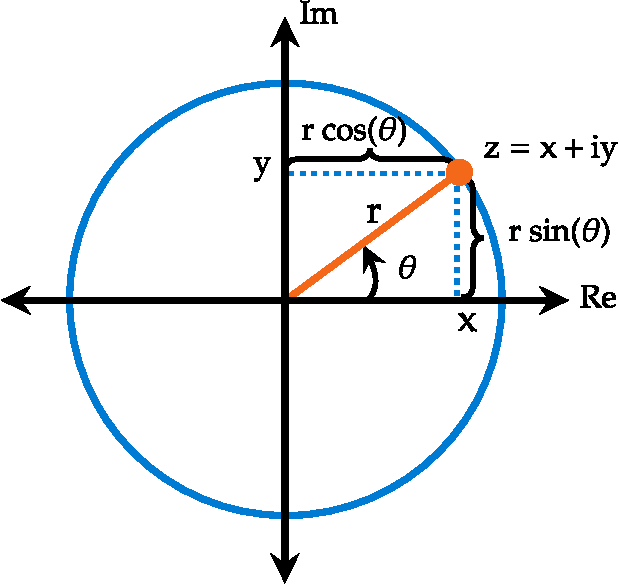
\includegraphics[width=0.30\textwidth]{cn1}
				\end{center}
			\caption{Argand Diagram}
			\label{Argand Diagram}
	    \end{figure}
    In terms of the polar coordinates  , we have
    \begin{align}
    x&=r \cos \theta, \quad y=r \sin \theta\\
    z&=x+\text { iy }=re^{i\theta} \notag \\&=r(\cos \theta+i \sin \theta)
    \label{Euler's equation}
    \end{align}
    Then, the  equation \ref{Euler's equation} is known as, Euler's formula
    \begin{figure}[H]
    	\begin{minipage}{0.40\textwidth}
    		\begin{center}
    		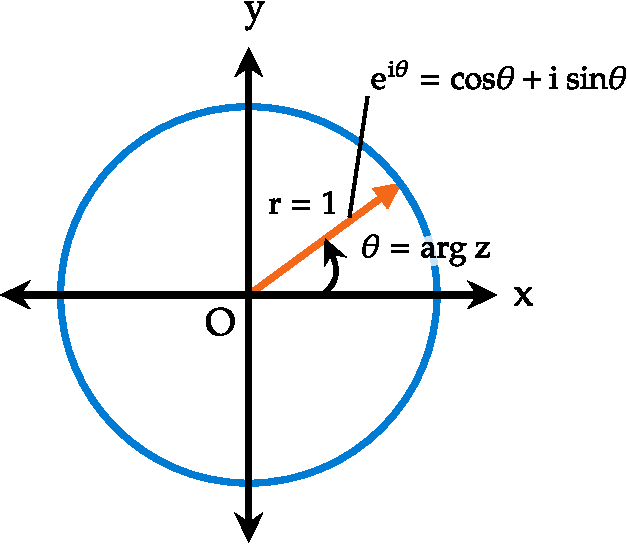
\includegraphics[width=0.70\textwidth]{cn2}
    	\end{center}
    	\end{minipage}\hfil
    	\begin{minipage}{0.40\textwidth}
    	\begin{center}
    		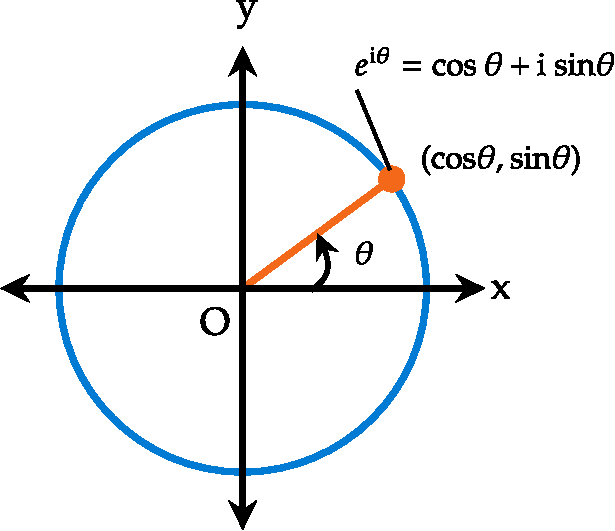
\includegraphics[width=0.70\textwidth]{cn3}
    	\end{center}
    \end{minipage}
    
    \caption{Polar representation}
    \end{figure}
   \subsection{Absolute Value}
    We define the absolute value of a complex number $x+i y$ to be the length ${r}$ of the vector from the origin to $P(x, y)$. 
    $$
    r=|x+i y|=\sqrt{x^{2}+y^{2}}
    $$
    \\\textbf{Properties:}
    \begin{itemize}
    	\item $\left|z_{1}+z_{2}\right| \leq\left|z_{1}\right|+\left|z_{2}\right|$
    	\item $\left|z_{1}-z_{2}\right| \geq\left|z_{1}\right|-\left|z_{2}\right|$
    	\item $\left|z_{1} z_{2}\right|=\left|z_{1}\right|\left|z_{2}\right|$
    	\item $\left|\frac{z_{1}}{z_{2}}\right|=\frac{\left|z_{1}\right|}{\left|z_{2}\right|}$
    \end{itemize}
    \subsection{Argument of $\mathbf{z}$ }
    The polar angle $\theta$ is called the {argument} of $z$ and it is written as, $${\theta=\arg z }$$ Any integer multiple of $2 \pi$ may be added to $\theta$ to produce another appropriate  angle.\\From the figure \ref{Argand Diagram},
    $${\theta=\arg z }=\tan ^{-1}\left(\frac{y}{x}\right)$$
    \\\textbf{Properties:}
    \begin{itemize}
    	\item $\operatorname{Arg}\left(z_{1}  z_{2} \cdot z_{3} \ldots \ldots z_{n}\right)=\operatorname{Arg} \left(z_{1}\right)+\operatorname{Arg}  \left(z_{2}\right)+\operatorname{Arg}  \left(z_{3}\right)+\ldots \ldots . .+\operatorname{Arg}\left(z_{n}\right)$
    	\item $\operatorname{Arg}\left(\frac{z_{1}}{z_{2}}\right)=\operatorname{Arg}\left(z_{1}\right)-\operatorname{Arg}\left(z_{2}\right)$
    \end{itemize}
\begin{exercise}
	Find the modulus and principal argument of the complex number
	$\frac{1+2 i}{1-(1-i)^{2}}$
\end{exercise}
\begin{answer}
	\begin{align*}
	\frac{1+2 i}{1-(1-i)^{2}}&=\frac{1+2 i}{1-(1-1-2 i)}=\frac{1+2 i}{1+2 i}\\&=1=1+0 i \\
	\therefore \quad\left|\frac{1+2 i}{1-(1-i)^{2}}\right|&=|1+0 i|=\sqrt{1^{2}}=1\\
	\text{Principal argument of}\ \frac{1+2 i}{1-(1-i)^{2}}&= \text{Principal argument of} \quad \left( 1+0 i\right) \\
	\tan ^{-1} \frac{0}{1}&=\tan ^{-1} 0\\&=0^{\circ}
	\end{align*}
\end{answer}

     \subsection{Conjugate of a Complex number}
	The conjugate of a complex number $z$ is represented by, $${\bar{z}=x-i y}$$
	\begin{note}\newline 
	$ \left. \right. $ \hspace{1.5cm}	$\begin{aligned}
		\frac{z + \bar{z}}{2}&=Re\left\lbrace z\right\rbrace \\
		\frac{z - \bar{z}}{2i}&=Im\left\lbrace z\right\rbrace\\
		z \cdot \bar{z}&=|z|^{2}
		\end{aligned}$
	\end{note}

\section{Algebra of Complex numbers}
For two Complex numbers, $a+i b$ and $c+i d $
\subsubsection{Equality:}
	\begin{align*}
	a+i b&=c+i d \quad
	\end{align*}
	Two complex numbers $(a, b)$
 and $(c, d)$ are equal if and only $a=c$ and $b=d$.
 \subsubsection{Addition:} 
 \begin{align*}
 (a+i b)+(c+i d) \quad&=(a+c)+i(b+d) \quad
 \end{align*}
 \subsubsection{Multiplication:} \begin{align*}
 (a+i b)(c+i d) &=(a c-b d)+i(a d+b c) \\
 c(a+i b)&=a c+i(b c)
 \end{align*}
 \textbf{Polar form:} 
 \begin{align*} 
 \text{Let,} \quad z_{1}&=r_{1}\left(\cos \theta_{1}+i \sin \theta_{1}\right) \quad \text{and}\quad z_{2}=r_{2}\left(\cos \theta_{2}+i \sin \theta_{2}\right)\\
 z_{1} . z_{2} &=r_{1} r_{2}\left(\cos \theta_{1}+i \sin \theta_{1}\right)\left(\cos \theta_{2}+i \sin \theta_{2}\right) \\ &=r_{1} r_{2}\left[\cos \theta_{1} \cos \theta_{2}-\sin \theta_{1} \sin \theta_{2}+i\left(\sin \theta_{1} \cos \theta_{2}+\cos \theta_{1} \sin \theta_{2}\right)\right] \\ &=r_{1} r_{1}\left[\cos \left(\theta_{1}+\theta_{2}\right)+i \sin \left(\theta_{1}+\theta_{2}\right)\right], \end{align*}
 
 \subsubsection{Division:}\begin{align*}
 \frac{c+i d}{a+i b}&=\frac{(c+i d)(a-i b)}{(a+i b)(a-i b)}\\&=\frac{(a c+b d)+i(a d-b c)}{a^{2}+b^{2}}\\
 \text{Where,}\quad x&=\frac{a c+b d}{a^{2}+b^{2}},\quad \text{and} \quad y=\frac{a d-b c}{a^{2}+b^{2}}
 \end{align*}
 \textbf{Polar form:}\\ Let $z_{1}=r_{1}\left(\cos \theta_{1}+i \sin \theta_{1}\right)$ and $z_{2}=r_{2}\left(\cos \theta_{2}+i \sin \theta_{2}\right)$\\\\\\
 $\begin{aligned} \frac{z_{1}}{z_{2}} &=\frac{r_{1}\left(\cos \theta_{1}+i \sin \theta_{1}\right)}{r_{2}\left(\cos \theta_{2}+i \sin \theta_{2}\right)}\\\\&=\frac{r_{1}\left(\cos \theta_{1}+i \sin \theta_{1}\right)\left(\cos \theta_{2}-i \sin \theta_{2}\right)}{r_{2}\left(\cos \theta_{2}+i \sin \theta_{2}\right)\left(\cos \theta_{2}-i \sin \theta_{2}\right)} \\\\ &=\frac{r_{1}\left[\left(\cos \theta_{1} \cos \theta_{2}+\sin \theta_{1} \sin \theta_{2}\right)+i\left(\sin \theta_{1} \cos \theta_{2}-\sin \theta_{2} \cos \theta_{1}\right)\right]}{r_{2}\left(\cos ^{2} \theta_{2}+\sin ^{2} \theta_{2}\right)} \\ &=\frac{r_{1}}{r_{2}}\left[\cos \left(\theta_{1}-\theta_{2}\right)+i \sin \left(\theta_{1}-\theta_{2}\right)\right] \end{aligned}$
\begin{exercise}
	Find
	\begin{enumerate}
		\item $(2+3 i)+(6-2 i)$
		\item $(2+3 i)-(6-2 i) $
		\item $(2+3 i)(6-2 i)$
		\item $\frac{2+3 i}{6-2 i}$
	\end{enumerate}
\end{exercise}
\begin{answer}\hspace{0.5cm}
		\begin{enumerate}
		\item $(2+3 i)+(6-2 i)=(2+6)+(3-2) i=8+i $
		
		\item $(2-6)+(3-(-2)) i=-4+5 i $
		\item
		\begin{align*}
		(2+3 i)(6-2 i)&=(2)(6)+(2)(-2 i)+(3 i)(6)+(3 i)(-2 i)\\
		&=12-4 i+18 i-6 i^{2}\\&=12+14 i+6=18+14 i
		\end{align*}
		\item 
		\begin{align*}
		\frac{2+3 i}{6-2 i}&=\frac{2+3 i}{6-2 i} \frac{6+2 i}{6+2 i}\\
		&=\frac{12+4 i+18 i+6 i^{2}}{36+12 i-12 i-4 i^{2}}\\
		&=\frac{6+22 i}{40}\\&=\frac{3}{20}+\frac{11}{20} i
		\end{align*}
	\end{enumerate}
\end{answer}
\begin{exercise}
	Express $\frac{(6+i) \cdot(2-i)}{(4+3 i) \cdot(1-2 i)}$ in the form of $a+i b$
\end{exercise}
\begin{answer}
	\begin{align*} \frac{(6+i) \cdot(2-i)}{(4+3 i) \cdot(1-2 i)} &=\frac{12+1+i(2-6)}{4+6+i(3-8)}=\frac{13-4 i}{10-5 i} \\ &=\frac{(13-4 i)(10+5 i)}{(10-5 i)(10+5 i)}=\frac{150+25 i}{100+25}\\&=\frac{6+i}{5}\\&=\frac{6}{5}+\frac{1}{5} i \end{align*}
\end{answer}


\section{Important Identities}
\subsection{Circular functions of Complex numbers}

\begin{align*}
	\bullet\quad\sin \theta=\frac{e^{i \theta}-e^{-i \theta}}{2 i}\quad\bullet&\quad\cos \theta=\frac{e^{i \theta}+e^{-i \theta}}{2}\\\\
\bullet\quad\sin z=\frac{e^{i z}-e^{-i z}}{2 i}\quad\bullet&\quad\cos z=\frac{e^{i z}+e^{-i z}}{2}
\end{align*}

\subsection{Hyperbolic functions of Complex numbers}
\begin{alignat*}{2}
&\bullet\quad \sinh x=\frac{e^{x}-e^{-x}}{2}\quad&&\bullet\quad \cosh x=\frac{e^{x}+e^{-x}}{2}\\
&\bullet\quad\tanh x=\frac{e^{x}-e^{-x}}{e^{x}+e^{-x}}\quad&&\bullet \quad {\coth} x=\frac{e^{x}+e^{-x}}{e^{x}-e^{-x}}
\\
&\bullet\quad{\operatorname{sech}} x=\frac{2}{e^{x}+e^{-x}} \quad&&\bullet \quad {\operatorname{cosech}} x=\frac{2}{e^{x}-e^{-x}}\\
&\bullet\quad\cosh x+\sinh x=\frac{e^{x}+e^{-x}}{2}+\frac{e^{x}-e^{-x}}{2}=e^{x} \quad&& \quad
\end{alignat*}
\begin{note}
\textbf{\textbf{Relation between Circular and Hyperbolic functions:}}\\\\
$\begin{array}{ll}\bullet\quad\sin i x=i \sinh x & \bullet\quad \sinh i x=i \sin x \\ \bullet\quad\cos i x=\cosh x & \bullet\quad \cosh i x=\cos x \\ \bullet\quad\tan i x=i \tanh x& \bullet\quad \tanh i x=i \tan x\end{array}$

\end{note}

\begin{theorem}
	\textbf{De Moivre's Theorem:}
	\begin{enumerate}
		\item For any integer $n,$ $(\cos \theta+i \sin \theta)^{n}=\cos n \theta+i \sin n \theta$
		\item 	If $n$ is a fraction, then $(\cos n \theta+i \sin n \theta)$ is one of the values .
	\end{enumerate}
\end{theorem}
\begin{exercise}
  Express $\frac{(\cos \theta+i \sin \theta)^{8}}{(\sin \theta+i \cos \theta)^{4}}$ in the form $(x+i y)$
\end{exercise}
\begin{answer}
	$$
	\begin{aligned}
	\frac{(\cos \theta+i \sin \theta)^{8}}{(\sin \theta+i \cos \theta)^{4}}=&\frac{(\cos \theta+i \sin \theta)^{8}}{(i)^{4}\left(\cos \theta+\frac{1}{i} \sin \theta\right)^{4}} \\
	=& \frac{(\cos \theta+i \sin \theta)^{8}}{(\cos \theta-i \sin \theta)^{4}}=\frac{(\cos \theta+i \sin \theta)^{8}}{[\cos (-\theta)+i \sin (-\theta)]^{4}} \\
	=& \frac{(\cos \theta+i \sin \theta)^{8}}{\left[(\cos \theta+i \sin \theta)^{-1}\right]^{4}}=\frac{(\cos \theta+i \sin \theta)^{8}}{(\cos \theta+i \sin \theta)^{-4}}=(\cos \theta+i \sin \theta)^{12} \\
	=& \cos 12 \theta+i \sin 12 \theta
	\end{aligned}
	$$
\end{answer}
\begin{note}
	Series expansion of different functions
	
	\begin{align*}
	e^{x}&=1+x+\frac{x^{2}}{2 !}+\frac{x^{3}}{3 !}+\frac{x^{4}}{4 !}+\ldots \\
	\sin x&=x-\frac{x^{3}}{3 !}+\frac{x^{5}}{5 !}-\frac{x^{7}}{7 !}+\ldots \\
	\cos x&=1-\frac{x^{2}}{2 !}+\frac{x^{4}}{4 !}-\frac{x^{6}}{6 !}+\ldots \\
	\tan x&=x+\frac{x^{3}}{3}+\frac{2 x^{5}}{15}+\frac{17 x^{7}}{315}+\frac{62 x^{9}}{2835} +\cdots\\
	\ln (1+x)&=x-\frac{x^{2}}{2}+\frac{x^{3}}{3}-\frac{x^{4}}{4}+\ldots \\
    \tan ^{-1}(x)&=x-\frac{x^{3}}{3}+\frac{x^{5}}{5}-\frac{x^{7}}{7}+\ldots
	\end{align*}
	
\end{note}
\newpage
\begin{abox}
	Practise Set-1
	\end{abox}
\begin{enumerate}[label=\color{ocre}\textbf{\arabic*.}]
	\item The value of the integral $\int_{C} d z z^{2} e^{z}$, where $C$ is an open contour in the complex $z$-plane as shown in the figure below, is:
	{\exyear{NET/JRF(JUNE-2011)}}
	\begin{figure}[H]
		\centering
		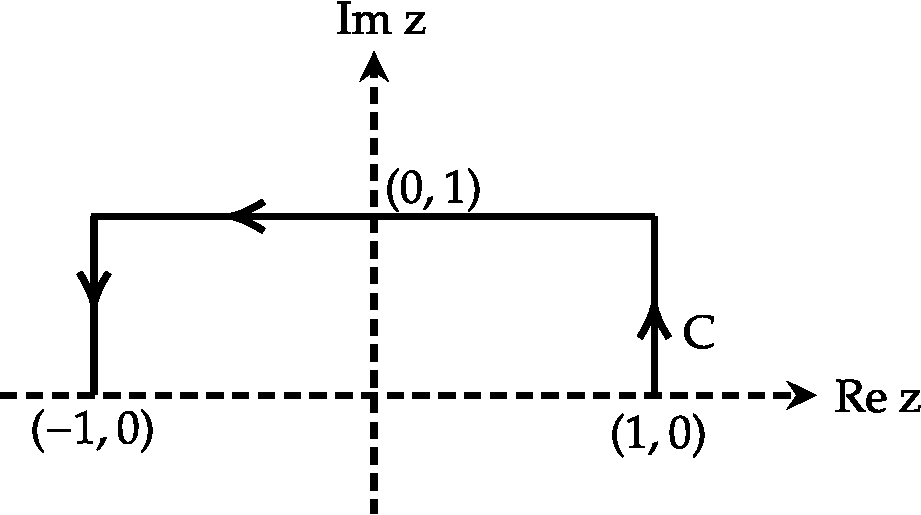
\includegraphics[height=5cm,width=9cm]{diagram-20211005-crop}
	\end{figure}
	\begin{tasks}(4)
		\task[\textbf{A.}] $\frac{5}{e}+e$
		\task[\textbf{B.}] $e-\frac{5}{e}$
		\task[\textbf{C.}] $\frac{5}{e}-e$
		\task[\textbf{D.}] $-\frac{5}{e}-e$
	\end{tasks}
	\item Which of the following is an analytic function of the complex variable $z=x+i y$ in the domain $|z|<2 ?$
	{\exyear{NET/JRF(JUNE-2011)}}
	\begin{tasks}(2)
		\task[\textbf{A.}] $(3+x-i y)^{7}$
		\task[\textbf{B.}] $(1+x+i y)^{4}(7-x-i y)^{3}$
		\task[\textbf{C.}] $(1-x-i y)^{4}(7-x+i y)^{3}$
		\task[\textbf{D.}] $(x+i y-1)^{1 / 2}$
	\end{tasks}
	\item The first few terms in the Laurent series for $\frac{1}{(z-1)(z-2)}$ in the region $1 \leq|z| \leq 2$ and around $z=1$ is
	{\exyear{NET/JRF(JUNE-2012)}}
	\begin{tasks}(1)
		\task[\textbf{A.}] $\frac{1}{2}\left[1+z+z^{2}+\ldots\right]\left[1+\frac{z}{2}+\frac{z^{2}}{4}+\frac{z^{3}}{8}+\ldots .\right]$
		\task[\textbf{B.}] $\frac{1}{1-z}-z-(1-z)^{2}+(1-z)^{3}+\ldots .$
		\task[\textbf{C.}] $\frac{1}{\mathrm{z}^{2}}\left[1+\frac{1}{\mathrm{z}}+\frac{1}{\mathrm{z}^{2}}+\ldots .\right]\left[1+\frac{2}{\mathrm{z}}+\frac{4}{\mathrm{z}^{2}}+\ldots . .\right]$
		\task[\textbf{D.}]  $2(z-1)+5(z-1)^{2}+7(z-1)^{3}+\ldots$
	\end{tasks}
	\item Let $u(x, y)=x+\frac{1}{2}\left(x^{2}-y^{2}\right)$ be the real part of analytic function $f(z)$ of the complex variable $z=x+i y$. The imaginary part of $f(z)$ is
	{\exyear{NET/JRF(JUNE-2012)}}
	\begin{tasks}(4)
		\task[\textbf{A.}] $y+x y$
		\task[\textbf{B.}] $x y$
		\task[\textbf{C.}] $y$
		\task[\textbf{D.}] $y^{2}-x^{2}$
	\end{tasks}
	\item The value of the integral $\int_{C} \frac{z^{3} d z}{\left(z^{2}-5 z+6\right)}$, where $C$ is a closed contour defined by the equation $2|z|-5=0$, traversed in the anti-clockwise direction, is
	{\exyear{NET/JRF(DEC-2012)}}
	\begin{tasks}(4)
		\task[\textbf{A.}] $-16 \pi i$
		\task[\textbf{B.}] $16 \pi \mathrm{i}$
		\task[\textbf{C.}] $8 \pi i$
		\task[\textbf{D.}] $2 \pi i$
	\end{tasks}
	\item  With $z=x+i y$, which of the following functions $f(x, y)$ is NOT a (complex) analytic function of $z$ ?
	{\exyear{NET/JRF(JUNE-2013)}}
	\begin{tasks}(1)
		\task[\textbf{A.}] $f(x, y)=(x+i y-8)^{3}\left(4+x^{2}-y^{2}+2 i x y\right)^{7}$
		\task[\textbf{B.}] $f(x, y)=(x+i y)^{7}(1-x-i y)^{3}$
		\task[\textbf{C.}] $f(x, y)=\left(x^{2}-y^{2}+2 i x y-3\right)^{5}$
		\task[\textbf{D.}] $f(x, y)=(1-x+i y)^{4}(2+x+i y)^{6}$
	\end{tasks}
	\item  Which of the following functions cannot be the real part of a complex analytic function of $z=x+i y ?$
	{\exyear{NET/JRF(DEC-2013)}}
	\begin{tasks}(4)
		\task[\textbf{A.}] $x^{2} y$
		\task[\textbf{B.}]  $x^{2}-y^{2}$
		\task[\textbf{C.}] $x^{3}-3 x y^{2}$
		\task[\textbf{D.}] $3 x^{2} y-y-y^{3}$
	\end{tasks}
	\item  Given that the integral $\int_{0}^{\infty} \frac{d x}{y^{2}+x^{2}}=\frac{\pi}{2 y}$, the value of $\int_{0}^{\infty} \frac{d x}{\left(y^{2}+x^{2}\right)^{2}}$ is
	{\exyear{NET/JRF(DEC-2013)}}
	\begin{tasks}(4)
		\task[\textbf{A.}] $\frac{\pi}{y^{3}}$
		\task[\textbf{B.}] $\frac{\pi}{4 y^{3}}$
		\task[\textbf{C.}]  $\frac{\pi}{8 y^{3}}$
		\task[\textbf{D.}] $\frac{\pi}{2 y^{3}}$
	\end{tasks}
	\item If $C$ is the contour defined by $|z|=\frac{1}{2}$, the value of the integral
	$$
	\oint_{C} \frac{d z}{\sin ^{2} z}
	$$
	is
	{\exyear{NET/JRF(JUNE-2014)}}
	\begin{tasks}(4)
		\task[\textbf{A.}] $\infty$
		\task[\textbf{B.}] $2 \pi i$
		\task[\textbf{C.}] 0
		\task[\textbf{D.}] $\pi i$
	\end{tasks}
	\item The principal value of the integral $\int_{-\infty}^{\infty} \frac{\sin (2 x)}{x^{3}} d x$ is
	{\exyear{NET/JRF(DEC-2014)}}
	\begin{tasks}(4)
		\task[\textbf{A.}] $-2 \pi$
		\task[\textbf{B.}]  $-\pi$
		\task[\textbf{C.}] $\pi$
		\task[\textbf{D.}]  $2 \pi$
	\end{tasks}
	\item The Laurent series expansion of the function $f(z)=e^{2}+e^{1 / 2}$ about $z=0$ is given by
	{\exyear{NET/JRF(DEC-2014)}}
	\begin{tasks}(2)
		\task[\textbf{A.}] $\sum_{n=-\infty}^{\infty} \frac{z^{n}}{n !}$ for all $|z|<\infty$
		\task[\textbf{B.}] $\sum_{n=0}^{\infty}\left(z^{n}+\frac{1}{z^{n}}\right) \frac{1}{n !}$ only if $0<|z|<1$
		\task[\textbf{C.}] $\sum_{n=0}^{\infty}\left(z^{n}+\frac{1}{z^{n}}\right) \frac{1}{n !}$ for all $0<|z|<\infty$
		\task[\textbf{D.}]  $\sum_{n=-\infty}^{\infty} \frac{z^{n}}{n !}$ only if $|z|<1$
	\end{tasks}
	\item Consider the function $f(z)=\frac{1}{z} \ln (1-z)$ of a complex variable $z=r e^{i \theta}(r \geq 0, \quad-\infty<\theta<\infty)$. The singularities of $f(z)$ are as follows:
	{\exyear{NET/JRF(DEC-2014)}}
	\begin{tasks}(1)
		\task[\textbf{A.}]  Branch points at $z=1$ and $z=\infty$; and a pole at $z=0$ only for $0 \leq \theta<2 \pi$
		\task[\textbf{B.}] Branch points at $z=1$ and $z=\infty$; and a pole at $z=0$ for all $\theta$ other than $0 \leq \theta<2 \pi$
		\task[\textbf{C.}] Branch points at $z=1$ and $z=\infty$; and a pole at $z=0$ for all $\theta$
		\task[\textbf{D.}] Branch points at $z=0, z=1$ and $z=\infty$.
	\end{tasks}
	\item  The value of integral $\int_{-\infty}^{\infty} \frac{d x}{1+x^{4}}$
	{\exyear{NET/JRF(JUNE-2015)}}
	\begin{tasks}(4)
		\task[\textbf{A.}] $\frac{\pi}{\sqrt{2}}$
		\task[\textbf{B.}] $\frac{\pi}{2}$
		\task[\textbf{C.}] $\sqrt{2} \pi$
		\task[\textbf{D.}] $2 \pi$
	\end{tasks}
	\item  The function $\frac{Z}{\sin \pi z^{2}}$ of a complex variable $z$ has
	{\exyear{NET/JRF(DEC-2015)}}
	\begin{tasks}(1)
		\task[\textbf{A.}] A simple pole at 0 and poles of order 2 at $\pm \sqrt{n}$ for $n=1,2,3 \ldots$
		\task[\textbf{B.}] A simple pole at 0 and poles of order 2 at $\pm \sqrt{n}$ and $\pm i \sqrt{n}$ for $n=1,2,3 \ldots$
		\task[\textbf{C.}] Poles of order 2 at $\pm \sqrt{n}, n=0,1,2,3 \ldots$
		\task[\textbf{D.}] Poles of order 2 at $\pm n, n=0,1,2,3 \ldots$
	\end{tasks}
	\item The value of the contour integral $\frac{1}{2 \pi i} \oint_{C} \frac{e^{4 z}-1}{\cosh (z)-2 \sinh (z)} d z$ around the unit circle $C$ traversed in the anti-clockwise direction, is
	{\exyear{NET/JRF(JUNE-2016)}}
	\begin{tasks}(4)
		\task[\textbf{A.}] 0
		\task[\textbf{B.}] 2
		\task[\textbf{C.}] $\frac{-8}{\sqrt{3}}$
		\task[\textbf{D.}] $-\tanh \left(\frac{1}{2}\right)$
	\end{tasks}
	\item  Let $u(x, y)=e^{a x} \cos (b y)$ be the real part of a function $f(z)=u(x, y)+i v(x, y)$ of the complex variable $z=x+i y$, where $a, b$ are real constants and $a \neq 0 .$ The function $f(z)$ is complex analytic everywhere in the complex plane if and only if
	{\exyear{NET/JRF(JUNE-2017)}}
	\begin{tasks}(4)
		\task[\textbf{A.}] $b=0$
		\task[\textbf{B.}] $b=\pm a$
		\task[\textbf{C.}] $b=\pm 2 \pi a$
		\task[\textbf{D.}]  $b=a \pm 2 \pi$
	\end{tasks}
	\item  The integral $\oint_{\Gamma} \frac{z e^{i \pi z / 2}}{z^{2}-1} d z$ along the closed contour $\Gamma$ shown in the figure is
	{\exyear{NET/JRF(JUNE-2017)}}
	\begin{figure}[H]
		\centering
		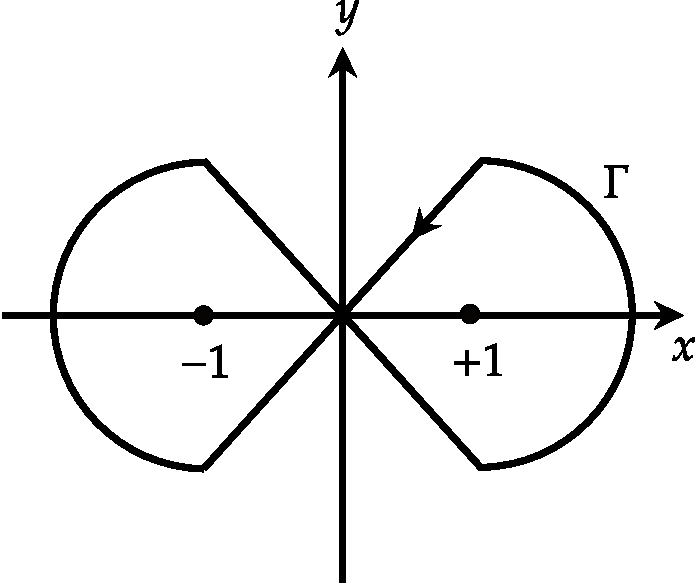
\includegraphics[height=4cm,width=5cm]{diagram-20211005(19)-crop}
	\end{figure}
	\begin{tasks}(4)
		\task[\textbf{A.}] 0
		\task[\textbf{B.}] $2 \pi$
		\task[\textbf{C.}] $-2 \pi$
		\task[\textbf{D.}] $4 \pi i$
	\end{tasks}
	\item What is the value of $a$ for which $f(x, y)=2 x+3\left(x^{2}-y^{2}\right)+2 i(3 x y+a y)$ is an analytic function of complex variable $z=x+i y$
	{\exyear{NET/JRF(JUNE-2018)}}
	\begin{tasks}(4)
		\task[\textbf{A.}] 1
		\task[\textbf{B.}] 0
		\task[\textbf{C.}] 3
		\task[\textbf{D.}] 2
	\end{tasks}
\item  The value of the integral $\oint_{C} \frac{d z}{z} \frac{\tanh 2 z}{\sin \pi z}$, where $C$ is a circle of radius $\frac{\pi}{2}$, traversed counter-clockwise, with centre at $z=0$, is
{\exyear{NET/JRF(DEC-2018)}}
\begin{tasks}(4)
	\task[\textbf{A.}] 4
	\task[\textbf{B.}] $4 i$
	\task[\textbf{C.}] $2 i$
	\task[\textbf{D.}] 0
\end{tasks}
	\item The integral $I=\int_{C} e^{z} d z$ is evaluated from the point $(-1,0)$ to $(1,0)$ along the contour $C$, which is an arc of the parabola $y=x^{2}-1$, as shown in the figure. The value of $I$ is
	{\exyear{NET/JRF(DEC-2018)}}
	\begin{figure}[H]
		\centering
		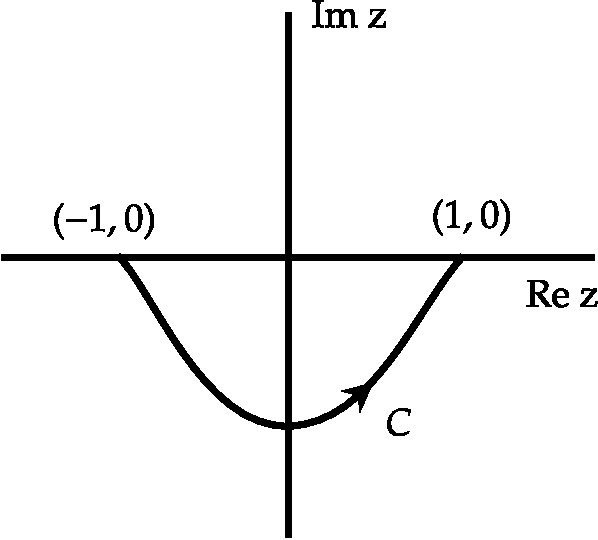
\includegraphics[height=4.5cm,width=5cm]{diagram-20211005(3)-crop}
	\end{figure}
	\begin{tasks}(4)
		\task[\textbf{A.}]  0
		\task[\textbf{B.}] $2 \sinh 1$
		\task[\textbf{C.}]  $e^{2 i} \sinh 1$
		\task[\textbf{D.}] $e+e^{-1}$
	\end{tasks}
	\item The contour $C$ of the following integral
	$$
	\oint_{C} d z \frac{\sqrt{(z-1)(z-3)}}{\left(z^{2}-25\right)^{3}}
	$$
	in the complex $z$ plane is shown in the figure below.\\
	\begin{figure}[H]
		\centering
		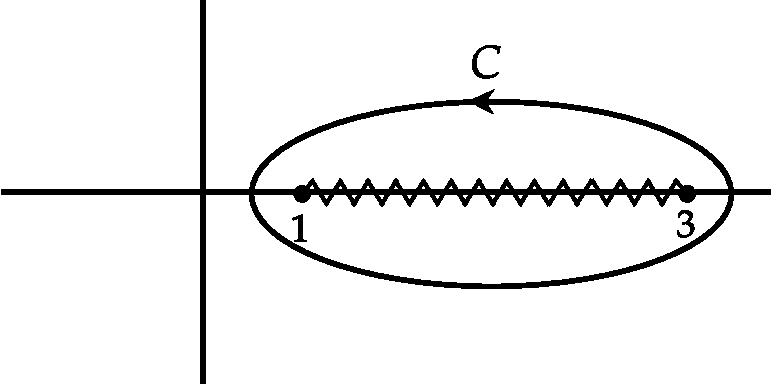
\includegraphics[height=3.5cm,width=6cm]{diagram-20211005(8)-crop}
	\end{figure}
	This integral is equivalent to an integral along the contours
	{\exyear{NET/JRF(DEC-2018)}}
	\begin{tasks}(2)
		\task[\textbf{A.}] \begin{figure}[H]
			\centering
			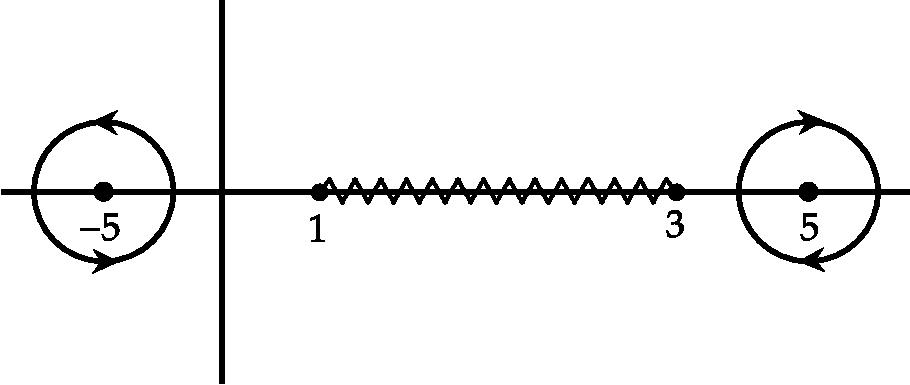
\includegraphics[height=3cm,width=6.5cm]{diagram-20211005(4)-crop}
		\end{figure}
		\task[\textbf{B.}] \begin{figure}[H]
			\centering
			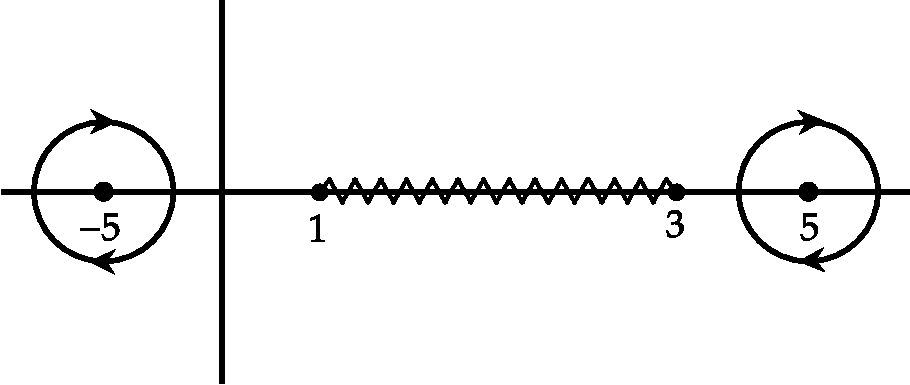
\includegraphics[height=3cm,width=6.5cm]{diagram-20211005(5)-crop}
		\end{figure}
		\task[\textbf{C.}] \begin{figure}[H]
			\centering
			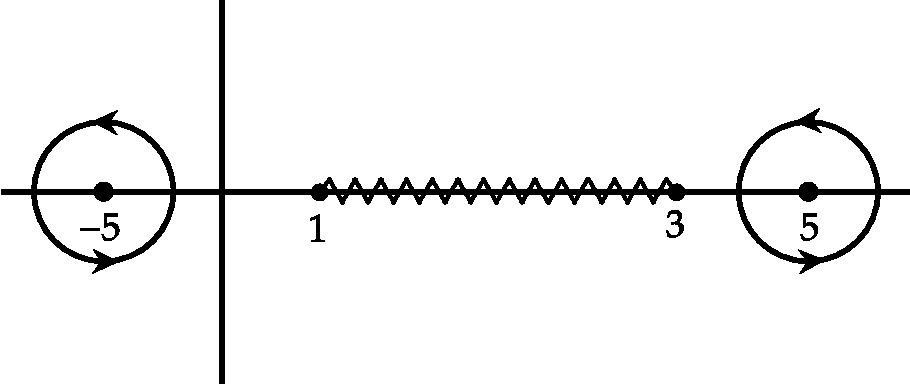
\includegraphics[height=3cm,width=6.5cm]{diagram-20211005(6)-crop}
		\end{figure}
		\task[\textbf{D.}] \begin{figure}[H]
			\centering
			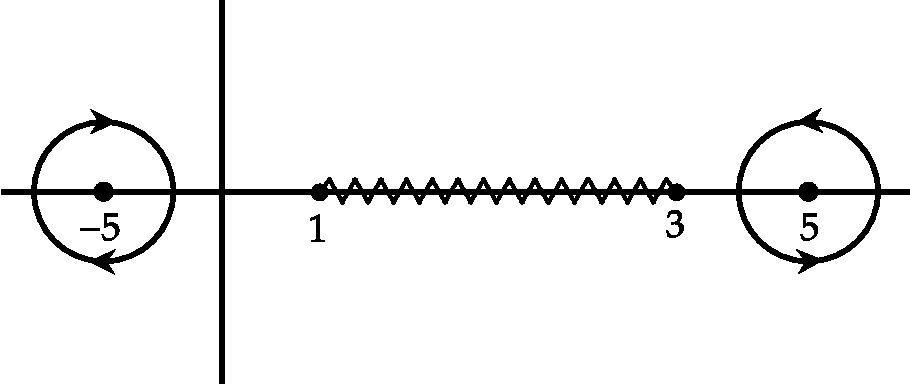
\includegraphics[height=3cm,width=6.5cm]{diagram-20211005(7)-crop}
		\end{figure}
	\end{tasks}
	\item  Let $C$ be the circle of radius $\frac{\pi}{4}$ centered at $z=\frac{1}{4}$ in the complex $z$-plane that is traversed counter-clockwise. The value of the contour integral $\oint_{C} \frac{z^{2}}{\sin ^{2} 4 z} d z$ is
	{\exyear{NET/JRF(DEC-2019)}}
	\begin{tasks}(4)
		\task[\textbf{A.}] 0
		\task[\textbf{B.}] $\frac{i \pi^{2}}{4}$
		\task[\textbf{C.}] $\frac{i \pi^{2}}{16}$
		\task[\textbf{D.}] $\frac{i \pi}{4}$
	\end{tasks}
	\item  A function of a complex variable $z$ is defined by the integral $f(z)=\oint_{\Gamma} \frac{w^{2}-2}{w-z} d w$, where $\Gamma$ is a circular contour of radius 3 , centred at origin, running counter-clockwise in the $w$ - plane. The value of the function at $z=(2-i)$ is
	{\exyear{NET/JRF(JUNE-2020)}}
	\begin{tasks}(4)
		\task[\textbf{A.}] 0
		\task[\textbf{B.}] $1-4 i$
		\task[\textbf{C.}]  $8 \pi+2 \pi \mathrm{i}$
		\task[\textbf{D.}] $-\frac{2}{\pi}-\frac{i}{2 \pi}$
	\end{tasks}
\end{enumerate}
 \colorlet{ocre1}{ocre!70!}
\colorlet{ocrel}{ocre!30!}
\setlength\arrayrulewidth{1pt}
\begin{table}[H]
	\centering
	\arrayrulecolor{ocre}
	\begin{tabular}{|p{1.5cm}|p{1.5cm}||p{1.5cm}|p{1.5cm}|}
		\hline
		\multicolumn{4}{|c|}{\textbf{Answer key}}\\\hline\hline
		\rowcolor{ocrel}Q.No.&Answer&Q.No.&Answer\\\hline
		1&\textbf{C} &2&\textbf{B}\\\hline 
		3&\textbf{B} &4&\textbf{A} \\\hline
		5&\textbf{A} &6&\textbf{D} \\\hline
		7&\textbf{A}&8&\textbf{-}\\\hline
		9&\textbf{C}&10&\textbf{A}\\\hline
		11&\textbf{C} &12&\textbf{-}\\\hline
		13&\textbf{A}&14&\textbf{B}\\\hline
		15&\textbf{C}&16&\textbf{B}\\\hline
		17&\textbf{C} &18&\textbf{A}\\\hline
		19&\textbf{B}&20&\textbf{B}\\\hline
		21&\textbf{C}&22&\textbf{C}\\\hline
		23&\textbf{C}& &\\\hline
		
	\end{tabular}
\end{table}
\newpage
\begin{abox}
	Practise Set-2
\end{abox}
\begin{enumerate}[label=\color{ocre}\textbf{\arabic*.}]
	\item  The value of the integral $\oint_{C} \frac{e^{z} \sin (z)}{z^{2}} d z$, where the contour $C$ is the unit circle: $|z-2|=1$, is
	{\exyear{GATE 2010}}
	\begin{tasks}(4)
		\task[\textbf{A.}] $2 \pi i$
		\task[\textbf{B.}] $4 \pi i$
		\task[\textbf{C.}] $\pi i$
		\task[\textbf{D.}] 0
	\end{tasks}
	\item Which of the following statements is TRUE for the function $f(z)=\frac{z \sin z}{(z-\pi)^{2}}$ ?
	{\exyear{GATE 2011}}
	\begin{tasks}(1)
		\task[\textbf{A.}] $f(z)$ is analytic everywhere in the complex plane
		\task[\textbf{B.}] $f(z)$ has a zero at $z=\pi$
		\task[\textbf{C.}] $f(z)$ has a pole of order 2 at $z=\pi$
		\task[\textbf{D.}] $f(z)$ has a simple pole at $z=\pi$
	\end{tasks}
	\item For the function $f(z)=\frac{16 z}{(z+3)(z-1)^{2}}$, the residue at the pole $z=1$ is (your answer should be an integer)-------
	{\exyear{GATE 2013}}
	\item The value of the integral
	$$
	\oint_{C} \frac{z^{2}}{e^{z}+1} d z
	$$
	where $C$ is the circle $|z|=4$, is
	{\exyear{GATE 2014}}
	\begin{tasks}(4)
		\task[\textbf{A.}] $2 \pi i$
		\task[\textbf{B.}] $2 \pi^{2} i$
		\task[\textbf{C.}]  $4 \pi^{3} i$
		\task[\textbf{D.}] $4 \pi^{2} i$
	\end{tasks}
	\item Consider a complex function $f(z)=\frac{1}{z\left(z+\frac{1}{2}\right) \cos (z \pi)}$. Which one of the following statements is correct?
	{\exyear{GATE 2015}}
	\begin{tasks}(1)
		\task[\textbf{A.}] $f(z)$ has simple poles at $z=0$ and $z=-\frac{1}{2}$
		\task[\textbf{B.}] $f(z)$ has second order pole at $z=-\frac{1}{2}$
		\task[\textbf{C.}] $f(z)$ has infinite number of second order poles
		\task[\textbf{D.}] $f(z)$ has all simple poles
	\end{tasks}
	\item  Consider $w=f(z)=u(x, y)+i v(x, y)$ to be an analytic function in a domain $D$. Which one of the following options is NOT correct?
	{\exyear{GATE 2015}}
	\begin{tasks}(1)
		\task[\textbf{A.}] $u(x, y)$ satisfies Laplace equation in D
		\task[\textbf{B.}]  $v(x, y)$ satisfies Laplace equation in $D$
		\task[\textbf{C.}] $\int_{1}^{z_{2}} f(z) d z$ is dependent on the choice of the contour between $z_{1}$ and $z_{2}$ in $D$
		\task[\textbf{D.}]  $f(z)$ can be Taylor expended in $D$
	\end{tasks}
	\item A function $y(z)$ satisfies the ordinary differential equation $y^{\prime \prime}+\frac{1}{z} y^{\prime}-\frac{m^{2}}{z^{2}} y=0$, where\\
	$m=0,1,2,3, \ldots . .$ Consider the four statements P, Q, R, S as given below.\\
	$\mathrm{P}: z^{m}$ and $z^{-m}$ are linearly independent solutions for all values of $m$\\
	Q: $z^{m}$ and $z^{-m}$ are linearly independent solutions for all values of $m>0$\\
	$\mathrm{R}$ : $\ln z$ and 1 are linearly independent solutions for $m=0$\\
	S: $z^{m}$ and $\ln z$ are linearly independent solutions for all values of $m$\\
	The correct option for the combination of valid statements is
	{\exyear{GATE 2015}}
	\begin{tasks}(4)
		\task[\textbf{A.}] P, R and S only
		\task[\textbf{B.}]  P and R only
		\task[\textbf{C.}] $\mathrm{Q}$ and $\mathrm{R}$ only
		\task[\textbf{D.}] $\mathrm{R}$ and $\mathrm{S}$ only
	\end{tasks}
	\item  Which of the following is an analytic function of $z$ everywhere in the complex plane?
	{\exyear{GATE 2016}}
	\begin{tasks}(4)
		\task[\textbf{A.}] $z^{2}$
		\task[\textbf{B.}]  $\left(z^{*}\right)^{2}$
		\task[\textbf{C.}] $|z|^{2}$
		\task[\textbf{D.}] $\sqrt{z}$
	\end{tasks}
	\item The contour integral $\oint \frac{d z}{1+z^{2}}$ evaluated along a contour going from $-\infty$ to $+\infty$ along the
	real axis and closed in the lower half-plane circle is equal to............... (up to two decimal places).
	{\exyear{GATE 2017}}
	\item The imaginary part of an analytic complex function is $v(x, y)=2 x y+3 y .$ The real part of the function is zero at the origin. The value of the real part of the function at $1+i$ is ................. (up to two decimal places)
	{\exyear{GATE 2017}}
	\item The absolute value of the integral
	$$
	\int \frac{5 z^{3}+3 z^{2}}{z^{2}-4} d z
	$$
	over the circle $|z-1.5|=1$ in complex plane, is $\ldots$ (up to two decimal places).
	{\exyear{GATE 2018}}
	\item The pole of the function $f(z)=\cot z$ at $z=0$ is
	{\exyear{GATE 2019}}
	\begin{tasks}(2)
		\task[\textbf{A.}] A removable pole
		\task[\textbf{B.}] An essential singularity
		\task[\textbf{C.}]  A simple pole
		\task[\textbf{D.}] A second order pole
	\end{tasks}
	\item The value of the integral $\int_{-\infty}^{\infty} \frac{\cos (k x)}{x^{2}+a^{2}} d x$, where $k>0$ and $a>0$, is
	{\exyear{GATE 2019}}
	\begin{tasks}(4)
		\task[\textbf{A.}] $\frac{\pi}{a} e^{-k a}$
		\task[\textbf{B.}] $\frac{2 \pi}{a} e^{-k a}$
		\task[\textbf{C.}] $\frac{\pi}{2 a} e^{-k a}$
		\task[\textbf{D.}] $\frac{3 \pi}{2 a} e^{-k a}$
	\end{tasks}
\end{enumerate}
 \colorlet{ocre1}{ocre!70!}
\colorlet{ocrel}{ocre!30!}
\setlength\arrayrulewidth{1pt}
\begin{table}[H]
	\centering
	\arrayrulecolor{ocre}
	\begin{tabular}{|p{1.5cm}|p{1.7cm}||p{1.5cm}|p{1.5cm}|}
		\hline
		\multicolumn{4}{|c|}{\textbf{Answer key}}\\\hline\hline
		\rowcolor{ocrel}Q.No.&Answer&Q.No.&Answer\\\hline
		1&\textbf{D} &2&\textbf{C}\\\hline 
		3&\textbf{3(NAT)} &4&\textbf{C} \\\hline
		5&\textbf{A} &6&\textbf{C} \\\hline
		7&\textbf{C}&8&\textbf{A}\\\hline
		9&\textbf{$\pi$(NAT)}&10&\textbf{3(NAT)}\\\hline
		11&\textbf{81.64(NAT)} &12&\textbf{C}\\\hline
		13&\textbf{A}& &\textbf{}\\\hline
		
	\end{tabular}
\end{table}
\newpage
\begin{abox}
	Practise Set-3
\end{abox}
\begin{enumerate}[label=\color{ocre}\textbf{\arabic*.}]
	\item Find the smallest positive integer $n$ for which
	$$
	\left(\frac{1+i}{1-i}\right)^{n}=1
	$$
	\begin{answer}
		\begin{align*}
		{\left[\frac{1+i}{1-i}\right]^{n}}&=1 \\
		{\left[\frac{1+i}{1-i} \times \frac{1+i}{1+i}\right]^{n}}&=1\\ \Rightarrow\left(\frac{1-1+2 i}{1+1}\right)^{n}&=1 \\
		(i)^{n}&=1=(i)^{4} \Rightarrow n=4
		\end{align*}
	
	\end{answer}
\item  Find the square root of the complex number $5+12 i$.

\begin{answer}
\begin{align}
\text{Let,}\quad \sqrt{5+12 i}&=x+i y \label{1}\\
\text{Squaring both sides of\quad \ref{1}}\quad \text{we get,}\notag\\
5+12 i=(x+i y)^{2}&=\left(x^{2}-y^{2}\right)+i 2 x y \label{2}\\
\text{Equating real and imaginary parts of \ref{2}}\notag\\
\text{we get,}\quad x^{2}-y^{2}&=5\label{3}\\
\text{and}\quad
2 x y &=12 \notag\\
x^{2}+y^{2} &=\sqrt{{({x^{2}-y^{2}})^{2}} +{4{x^{2}y^{2}}}}=\sqrt{(5)^{2}+(12)^{2}}\notag\\
&=\sqrt{25+144}=\sqrt{169}=13 \\
x^{2}+y^{2} &=13\label{4}\\
\text{adding}\quad\ref{3} \quad\text{and}\quad\ref{4}\quad\text{we get,}\notag\\
2 x^{2}=5+13=18 &\Rightarrow x=\sqrt{\frac{18}{2}}=\sqrt{9}=\pm 3\\
\text{subtracting}\quad\ref{3} \quad\text{by}\quad\ref{4}\quad\text{we get,}\notag\\
2 y^{2}=13-5=8 &\Rightarrow y=\sqrt{\frac{8}{2}}=\sqrt{4}=\pm 2\\
\text{since $ xy$ is positive,}&\text{ so $x$ and $y$ are of same sign}\notag \\
\text{Hence, $x=\pm 3, y=\pm 2$}\notag\\\therefore \sqrt{5+12 i}&=\pm 3 \pm 2 i \notag\\ i.e. \quad(3+2 i) &\text{or} -(3+2 i)\notag
\end{align}
\end{answer}
\item The value of $\frac{(\cos 3 \theta+i \sin 3 \theta)^{4}(\cos 4 \theta-i \sin 4 \theta)^{5}}{(\cos 4 \theta+i \sin 4 \theta)^{3}(\cos 5 \theta+i \sin 5 \theta)^{-4}}$ is
\begin{answer}
\begin{align*}
\text{We have, }
(\cos 3 \theta+i \sin 3 \theta)^{4}&=\cos 12 \theta+i \sin 12 \theta=(\cos \theta+i \sin \theta)^{12}\\
(\cos 4 \theta-i \sin 4 \theta)^{5}&=\cos 20 \theta-i \sin 20 \theta=(\cos \theta+i \sin \theta)^{-20} \\
(\cos 4 \theta+i \sin 4 \theta)^{3}&=\cos 12 \theta+i \sin 12 \theta=(\cos \theta+i \sin \theta)^{12}\\
(\cos 5 \theta+i \sin 5 \theta)^{-4}&=\cos 20 \theta-i \sin 20 \theta=(\cos \theta+i \sin \theta)^{-20}\\
\text{Hence the value of given expression is 1}
\end{align*}
\end{answer}
\item Write $i^{(1-i)}$ in the form $r(\cos \theta+i \sin \theta)$
\begin{answer}
	\begin{align*}
		i^{1-i} &=e^{\log i^{(1-i)}}=e^{(1-i) \log i} \\
		&=e^{(1-i) \log \left(\cos \frac{\pi}{2}+i \sin \frac{\pi}{2}\right)}\\
		&=e^{(1-i) \log \left\{\cos \left(2 n \pi+\frac{\pi}{2}\right)+i \sin \left(2 n \pi+\frac{\pi}{2}\right)\right\}} \\
		&=e^{(1-i)} \log e^{i\left(2 n \pi+\frac{\pi}{2}\right)} \\
		&=e^{(1-i) i\left(2 n \pi+\frac{\pi}{2}\right)}=e^{(i+1)\left(2 n \pi+\frac{\pi}{2}\right)} \\
		&=e^{i\left(2 n \pi+\frac{\pi}{2}\right)} \cdot e^{\left(2 n \pi+\frac{\pi}{2}\right)} \\
		&=\mathrm{e}^{\left(2 n \pi+\frac{\pi}{2}\right)}\left\{\cos \left(2 n \pi+\frac{\pi}{2}\right)+i \sin \left(2 n \pi+\frac{\pi}{2}\right)\right\} \\
		&=e^{\left(2 n \pi+\frac{\pi}{2}\right)} . i=i e^{\left(2 n \pi+\frac{\pi}{2}\right)}
	\end{align*}
\end{answer}
\item Find the general value of $\log (1+i)+\log (1-i)$
\begin{answer}
	\begin{align*}
	1+i&=\sqrt{2}\left(\frac{1}{\sqrt{2}}+\frac{i}{\sqrt{2}}\right)\\
		&=\sqrt{2}\left\{\cos \left(2 n+\frac{1}{4}\right) \pi+i \sin \left(2 n+\frac{1}{4}\right) \pi\right\} \\
		&=\sqrt{2} e^{\left(2 n+\frac{1}{4}\right) \pi} \\
		\log (1+i) &=\log \left\{\sqrt{2} e^{\left(2 n+\frac{1}{4}\right) \pi}\right\}=\log \sqrt{2}+i\left(2 n+\frac{1}{4}\right) \pi \\
		\operatorname{Similarly}(1-i) &=\sqrt{2} e^{+i\left(2 n-\frac{1}{4}\right) \pi} \\
		\log (1-i) &=\log \left\{\sqrt{2} e^{+i\left(2 n-\frac{1}{4} \pi\right)}=\log \sqrt{2}+i\left(2 n-\frac{1}{4}\right) \pi\right.\\
		\log (1+i)+\log (1-i) &=\log \sqrt{2}+i\left(2 n+\frac{1}{4}\right) \pi+\log \sqrt{2}+i\left(2 n-\frac{1}{4}\right) \pi \\
		&=2 \log \sqrt{2}+4 n \pi i=\log 2+4 n \pi i
	\end{align*}
\end{answer}
\item The point representing complex number for which $|z+4|^{2}-|z-4|^{2}=8$ lie on
\begin{tasks}(2)
	\task[\textbf{a.}]A straight line parallel to $x$ -axis.  
	\task[\textbf{b.}]A straight line parallel to $y$ -axis.
	\task[\textbf{c.}]A circle with centre as origin. 
	\task[\textbf{d.}]A circle with centre other than origin. 
\end{tasks}
\begin{answer}
	Let $z=x+i y,$ then
	$$
	|z+4|^{2}-|z-4|^{2}=8 \Rightarrow 4 \operatorname{Re}(4 z)=8
	$$
	where $\operatorname{Re}(4 z)$ is the real part of the complex number $4 z$
	\\$\Rightarrow \quad \operatorname{Re}(z)=\frac{1}{2} \Rightarrow x=\frac{1}{2},$ which is a straight line parallel to the $y$ -axis.\\Hence option(b)is correct.
\end{answer}
\item Given two complex numbers $z_{1}=5+(5 \sqrt{3}) i$ and
$z_{2}=\frac{z}{\sqrt{3}}+2 i,$ the argument of $\frac{z_{1}}{z_{2}}$ in degrees is
\begin{tasks}(4)
	\task[\textbf{a.}]0  
	\task[\textbf{b.}]30
	\task[\textbf{c.}]60 
	\task[\textbf{d.}]90 
\end{tasks}
\begin{answer}
	\begin{align*}
	z_{1}&=5+(5 \sqrt{3}) i\text{and} z_{2}=\frac{z}{\sqrt{3}}+2 i\\
	\arg z_{1}&=\tan ^{-1}\left(\frac{5 \sqrt{3}}{5}\right)=\tan ^{-1}(\sqrt{3})=60\\
	\arg z_{2}&=\tan ^{-1}\left(\frac{2}{\frac{2}{\sqrt{3}}}\right)=\tan ^{-1}(\sqrt{3})=60^{\circ}\\
	\arg \left(\frac{z_{1}}{z_{2}}\right)&=\arg \left(z_{1}\right)-\arg \left(z_{2}\right)=60^{\circ}-60^{\circ}=0
	\end{align*}
\end{answer}
\item If $z=x+i y$, then the realpart of $\cos (z)$ is 
\begin{tasks}(2)
	\task[\textbf{a.}]$\cos (x) \cosh (y)$  
	\task[\textbf{b.}]$\cos (x) \cos (y)$
	\task[\textbf{c.}] $\sin (x) \sinh (y)$ 
	\task[\textbf{d.}]$-\sin (x) \sinh (y)$ 
\end{tasks}
\begin{answer}
	\begin{align*}
	\cos z&=\cos (x+i y)=\cos x \cos i y-\sin x \sin i y\\&=\cos x \cosh y-i \sin x \sinh y
	\end{align*}
Therefore, real part is, $\cos x \cosh y$
\end{answer}
\item For the roots of unity $z=e^{2 \pi \frac{i}{m}}, m>1$. The value of $1+z+z^{2}+\cdots z^{m-1}$ is equal to
\begin{answer}
	\begin{align*}
1+z+z^{2}+\cdots z^{m-1}&=\frac{1-z^{m}}{1-z}\\\text{(sum of ' $m$ ' terms of G.P.)}\\
\text{Here, }z^{m}&=e^{2 \pi \frac{i}{m} \times m}=e^{2 \pi i}=1\\
\therefore \frac{1-z^{m}}{1-z}&=0
\\\text{Correct answer is (0)}
\end{align*}
\end{answer}
\item If $|z|=1,$ then for all complex numbers ' $a$ ' and $b$ ' value of $\left|\frac{a z+b}{\vec{b} z+\bar{a}}\right|$ is equal to
\begin{tasks}(4)
	\task[\textbf{a.}]$\sqrt{a^{2}+b^{2}}$  
	\task[\textbf{b.}]1
	\task[\textbf{c.}] $\frac{a}{b}$
    \task[\textbf{d.}]$\frac{b}{a}$  
\end{tasks}
\begin{answer}
	\begin{align*}
	\left|\frac{a z+b}{\bar{b} z+\bar{a}}\right|&=\frac{\left|z\left(a+\frac{b}{z}\right)\right|}{|\bar{b} z+\bar{a}|}=\frac{|z|\left|a+b z^{-1}\right|}{|\bar{b} z+\bar{a}|}\\&=\frac{|a+b \bar{z}|}{|\bar{b} z+\bar{a}|} \qquad\left[\because|z|=1, z \bar{z}=1, \bar{z}=z^{-1}\right]\\
	\text{Now, since }|\bar{z}|&=|z|\\
	|a+b \bar{z}|&=|\overline{a+b \bar{z}}|=|\bar{a}+\bar{b} \bar{z}|=|\bar{a}+\bar{b} z| \\
	\left|\frac{a z+b}{\bar{b} z+\bar{a}}\right|&=\frac{|a+b \bar{z}|}{|\bar{b} z+\bar{a}|}=\frac{|\bar{a}+\bar{b} z|}{|\bar{a}+\bar{b} z|}=1
	\end{align*}
	
	
\end{answer}
\end{enumerate}


%----------------------------------------------------------------------------------------
%	INDEX
%----------------------------------------------------------------------------------------

\cleardoublepage % Make sure the index starts on an odd (right side) page
\phantomsection
\setlength{\columnsep}{0.75cm} % Space between the 2 columns of the index
\addcontentsline{toc}{chapter}{\textcolor{ocre}{Index}} % Add an Index heading to the table of contents


%----------------------------------------------------------------------------------------

\end{document}
